%&preformat-disser
\RequirePackage[l2tabu,orthodox]{nag} % Раскомментировав, можно в логе получать рекомендации относительно правильного использования пакетов и предупреждения об устаревших и нерекомендуемых пакетах
% Формат А4, 14pt (ГОСТ Р 7.0.11-2011, 5.3.6)
\documentclass[a4paper,14pt,oneside,openany]{memoir}

%%%%%%%%%%%%%%%%%%%%%%%%%%%%%%%%%%%%%%%%%%%%%%%%%%%%%%%%%%%%%%%%%%%%%%%%%%%%%%%%
%%%% Файл упрощённых настроек шаблона, общих для диссертации и автореферата %%%%
%%%%%%%%%%%%%%%%%%%%%%%%%%%%%%%%%%%%%%%%%%%%%%%%%%%%%%%%%%%%%%%%%%%%%%%%%%%%%%%%

%%% Режим черновика %%%
\makeatletter
\@ifundefined{c@draft}{
  \newcounter{draft}
  \setcounter{draft}{0}  % 0 --- чистовик (максимальное соблюдение ГОСТ)
                         % 1 --- черновик (отклонения от ГОСТ, но быстрая
                         %       сборка итоговых PDF)
}{}
\makeatother

%%% Пометки в тексте %%%
\makeatletter
\@ifundefined{c@showmarkup}{
  \newcounter{showmarkup}
  \setcounter{showmarkup}{0}  % 0 --- скрыть пометки
                              % 1 --- показывать пометки
}{}
\makeatother

%%% Использование в pdflatex шрифтов не по-умолчанию %%%
\makeatletter
\@ifundefined{c@usealtfont}{
  \newcounter{usealtfont}
  \setcounter{usealtfont}{1}    % 0 --- шрифты на базе Computer Modern
                                % 1 --- использовать пакет pscyr, при его
                                %       наличии
                                % 2 --- использовать пакет XCharter, при наличии
                                %       подходящей версии
}{}
\makeatother

%%% Использование в xelatex и lualatex семейств шрифтов %%%
\makeatletter
\@ifundefined{c@fontfamily}{
  \newcounter{fontfamily}
  \setcounter{fontfamily}{1}  % 0 --- CMU семейство. Используется как fallback;
                              % 1 --- Шрифты от MS (Times New Roman и компания)
                              % 2 --- Семейство Liberation
}{}
\makeatother

%%% Библиография %%%
\makeatletter
\@ifundefined{c@bibliosel}{
  \newcounter{bibliosel}
  \setcounter{bibliosel}{0}   % 0 --- встроенная реализация с загрузкой файла
                              %       через движок bibtex8;
                              % 1 --- реализация пакетом biblatex через движок
                              %       biber
}{}
\makeatother

%%% Вывод типов ссылок в библиографии %%%
\makeatletter
\@ifundefined{c@mediadisplay}{
  \newcounter{mediadisplay}
  \setcounter{mediadisplay}{1}   % 0 --- не делать ничего; надписи [Текст] и
                                 %       [Эл. ресурс] будут выводиться только в ссылках с
                                 %       заполненным полем `media`;
                                 % 1 --- автоматически добавлять надпись [Текст] к ссылкам с
                                 %       незаполненным полем `media`; таким образом, у всех
                                 %       источников будет указан тип, что соответствует
                                 %       требованиям ГОСТ
                                 % 2 --- автоматически удалять надписи [Текст], [Эл. Ресурс] и др.;
                                 %       не соответствует ГОСТ
                                 % 3 --- автоматически удалять надпись [Текст];
                                 %       не соответствует ГОСТ
                                 % 4 --- автоматически удалять надпись [Эл. Ресурс];
                                 %       не соответствует ГОСТ
}{}
\makeatother

%%% Предкомпиляция tikz рисунков для ускорения работы %%%
\makeatletter
\@ifundefined{c@imgprecompile}{
  \newcounter{imgprecompile}
  \setcounter{imgprecompile}{0}   % 0 --- без предкомпиляции;
                                  % 1 --- пользоваться предварительно
                                  %       скомпилированными pdf вместо генерации
                                  %       заново из tikz
}{}
\makeatother
            % общие настройки шаблона
\input{common/packages}         % Пакеты общие для диссертации и автореферата
\synopsisfalse                      % Этот документ --- не автореферат
\input{Dissertation/dispackages}    % Пакеты для диссертации
\input{Dissertation/userpackages}   % Пакеты для специфических пользовательских задач

%%%%%%%%%%%%%%%%%%%%%%%%%%%%%%%%%%%%%%%%%%%%%%%%%%%%%%%%%%%%%%%%%%%%%%%%%%%%%%%%
%%%% Файл упрощённых настроек шаблона, общих для диссертации и автореферата %%%%
%%%%%%%%%%%%%%%%%%%%%%%%%%%%%%%%%%%%%%%%%%%%%%%%%%%%%%%%%%%%%%%%%%%%%%%%%%%%%%%%

%%% Режим черновика %%%
\makeatletter
\@ifundefined{c@draft}{
  \newcounter{draft}
  \setcounter{draft}{0}  % 0 --- чистовик (максимальное соблюдение ГОСТ)
                         % 1 --- черновик (отклонения от ГОСТ, но быстрая
                         %       сборка итоговых PDF)
}{}
\makeatother

%%% Пометки в тексте %%%
\makeatletter
\@ifundefined{c@showmarkup}{
  \newcounter{showmarkup}
  \setcounter{showmarkup}{0}  % 0 --- скрыть пометки
                              % 1 --- показывать пометки
}{}
\makeatother

%%% Использование в pdflatex шрифтов не по-умолчанию %%%
\makeatletter
\@ifundefined{c@usealtfont}{
  \newcounter{usealtfont}
  \setcounter{usealtfont}{1}    % 0 --- шрифты на базе Computer Modern
                                % 1 --- использовать пакет pscyr, при его
                                %       наличии
                                % 2 --- использовать пакет XCharter, при наличии
                                %       подходящей версии
}{}
\makeatother

%%% Использование в xelatex и lualatex семейств шрифтов %%%
\makeatletter
\@ifundefined{c@fontfamily}{
  \newcounter{fontfamily}
  \setcounter{fontfamily}{1}  % 0 --- CMU семейство. Используется как fallback;
                              % 1 --- Шрифты от MS (Times New Roman и компания)
                              % 2 --- Семейство Liberation
}{}
\makeatother

%%% Библиография %%%
\makeatletter
\@ifundefined{c@bibliosel}{
  \newcounter{bibliosel}
  \setcounter{bibliosel}{0}   % 0 --- встроенная реализация с загрузкой файла
                              %       через движок bibtex8;
                              % 1 --- реализация пакетом biblatex через движок
                              %       biber
}{}
\makeatother

%%% Вывод типов ссылок в библиографии %%%
\makeatletter
\@ifundefined{c@mediadisplay}{
  \newcounter{mediadisplay}
  \setcounter{mediadisplay}{1}   % 0 --- не делать ничего; надписи [Текст] и
                                 %       [Эл. ресурс] будут выводиться только в ссылках с
                                 %       заполненным полем `media`;
                                 % 1 --- автоматически добавлять надпись [Текст] к ссылкам с
                                 %       незаполненным полем `media`; таким образом, у всех
                                 %       источников будет указан тип, что соответствует
                                 %       требованиям ГОСТ
                                 % 2 --- автоматически удалять надписи [Текст], [Эл. Ресурс] и др.;
                                 %       не соответствует ГОСТ
                                 % 3 --- автоматически удалять надпись [Текст];
                                 %       не соответствует ГОСТ
                                 % 4 --- автоматически удалять надпись [Эл. Ресурс];
                                 %       не соответствует ГОСТ
}{}
\makeatother

%%% Предкомпиляция tikz рисунков для ускорения работы %%%
\makeatletter
\@ifundefined{c@imgprecompile}{
  \newcounter{imgprecompile}
  \setcounter{imgprecompile}{0}   % 0 --- без предкомпиляции;
                                  % 1 --- пользоваться предварительно
                                  %       скомпилированными pdf вместо генерации
                                  %       заново из tikz
}{}
\makeatother
      % Упрощённые настройки шаблона

% Новые переменные, которые могут использоваться во всём проекте
% ГОСТ 7.0.11-2011
% 9.2 Оформление текста автореферата диссертации
% 9.2.1 Общая характеристика работы включает в себя следующие основные структурные
% элементы:
% актуальность темы исследования;
\newcommand{\actualityTXT}{Актуальность темы.}
% степень ее разработанности;
\newcommand{\progressTXT}{Степень разработанности темы.}
% цели и задачи;
\newcommand{\aimTXT}{Целью}
\newcommand{\tasksTXT}{задачи}
% научную новизну;
\newcommand{\noveltyTXT}{Научная новизна:}
% теоретическую и практическую значимость работы;
%\newcommand{\influenceTXT}{Теоретическая и практическая значимость}
% или чаще используют просто
\newcommand{\influenceTXT}{Практическая значимость}
% методологию и методы исследования;
\newcommand{\methodsTXT}{Методология и методы исследования.}
% положения, выносимые на защиту;
\newcommand{\defpositionsTXT}{Основные положения, выносимые на~защиту:}
% степень достоверности и апробацию результатов.
\newcommand{\reliabilityTXT}{Достоверность}
\newcommand{\probationTXT}{Апробация работы.}

\newcommand{\contributionTXT}{Личный вклад.}
\newcommand{\publicationsTXT}{Публикации.}


%%% Заголовки библиографии:

% для автореферата:
\newcommand{\bibtitleauthor}{Публикации автора по теме диссертации}

% для стиля библиографии `\insertbiblioauthorgrouped`
\newcommand{\bibtitleauthorvak}{В изданиях из списка ВАК РФ}
\newcommand{\bibtitleauthorscopus}{В изданиях, входящих в международную базу цитирования Scopus}
\newcommand{\bibtitleauthorwos}{В изданиях, входящих в международную базу цитирования Web of Science}
\newcommand{\bibtitleauthorother}{В прочих изданиях}
\newcommand{\bibtitleauthorconf}{В сборниках трудов конференций}
\newcommand{\bibtitleauthorpatent}{Зарегистрированные патенты}
\newcommand{\bibtitleauthorprogram}{Зарегистрированные программы для ЭВМ}

% для стиля библиографии `\insertbiblioauthorimportant`:
\newcommand{\bibtitleauthorimportant}{Наиболее значимые \protect\MakeLowercase\bibtitleauthor}

% для списка литературы в диссертации и списка чужих работ в автореферате:
\newcommand{\bibtitlefull}{Список литературы} % (ГОСТ Р 7.0.11-2011, 4)

% короткая запись символа частной производной
\newcommand\p{\ensuremath{\partial\:\!}}
% короткая запись частной производной| \: - 4/18 fs, \! - -3/13 fs
\newcommand\pfrac[2]{\frac{\p#1}{\p#2}}
         % Новые переменные, для всего проекта

%%% Основные сведения %%%
\newcommand{\thesisAuthorLastName}{\fixme{Иващенко}}
\newcommand{\thesisAuthorOtherNames}{\fixme{Владислав Александрович}}
\newcommand{\thesisAuthorInitials}{\fixme{В.\,А.}}
\newcommand{\thesisAuthor}             % Диссертация, ФИО автора
{%
    \texorpdfstring{% \texorpdfstring takes two arguments and uses the first for (La)TeX and the second for pdf
        \thesisAuthorLastName~\thesisAuthorOtherNames% так будет отображаться на титульном листе или в тексте, где будет использоваться переменная
    }{%
        \thesisAuthorLastName, \thesisAuthorOtherNames% эта запись для свойств pdf-файла. В таком виде, если pdf будет обработан программами для сбора библиографических сведений, будет правильно представлена фамилия.
    }
}
\newcommand{\thesisAuthorShort}        % Диссертация, ФИО автора инициалами
{\thesisAuthorInitials~\thesisAuthorLastName}
%\newcommand{\thesisUdk}                % Диссертация, УДК
%{\fixme{xxx.xxx}}
\newcommand{\thesisTitle}              % Диссертация, название
{\fixme{Прямое численное моделирование сдвиговых течений переменной плотности}}
\newcommand{\thesisSpecialtyNumber}    % Диссертация, специальность, номер
{\fixme{01.02.05}}
\newcommand{\thesisSpecialtyTitle}     % Диссертация, специальность, название (название взято с сайта ВАК для примера)
{\fixme{Механика жидкости, газа и плазмы}}
%% \newcommand{\thesisSpecialtyTwoNumber} % Диссертация, вторая специальность, номер
%% {\fixme{XX.XX.XX}}
%% \newcommand{\thesisSpecialtyTwoTitle}  % Диссертация, вторая специальность, название
%% {\fixme{Теория и~методика физического воспитания, спортивной тренировки,
%% оздоровительной и~адаптивной физической культуры}}
\newcommand{\thesisDegree}             % Диссертация, ученая степень
{\fixme{кандидата физико-математических наук}}
\newcommand{\thesisDegreeShort}        % Диссертация, ученая степень, краткая запись
{\fixme{канд. физ.-мат. наук}}
\newcommand{\thesisCity}               % Диссертация, город написания диссертации
{\fixme{Новосибирск}}
\newcommand{\thesisYear}               % Диссертация, год написания диссертации
{\the\year}
\newcommand{\thesisOrganization}       % Диссертация, организация
{\fixme{Федеральное государственное бюджетное учреждение науки 
Институт теплофизики им. С.С. Кутателадзе 
Сибирского отделения Российской академии наук}}
\newcommand{\thesisOrganizationShort}  % Диссертация, краткое название организации для доклада
{\fixme{ИТ СО РАН}}

\newcommand{\thesisInOrganization}     % Диссертация, организация в предложном падеже: Работа выполнена в ...
{\fixme{Федеральном государственном бюджетном учреждении науки 
Институте теплофизики им. С.С. Кутателадзе 
Сибирского отделения Российской академии наук}}

%% \newcommand{\supervisorDead}{}           % Рисовать рамку вокруг фамилии
\newcommand{\supervisorFio}              % Научный руководитель, ФИО
{\fixme{Мулляджанов Рустам Илхамович}}
\newcommand{\supervisorRegalia}          % Научный руководитель, регалии
{\fixme{доктор физико-математических наук}}
\newcommand{\supervisorFioShort}         % Научный руководитель, ФИО
{\fixme{Р.\,И.~Мулляджанов}}
\newcommand{\supervisorRegaliaShort}     % Научный руководитель, регалии
{\fixme{д.ф.-м.н.}}

%% \newcommand{\supervisorTwoDead}{}        % Рисовать рамку вокруг фамилии
%% \newcommand{\supervisorTwoFio}           % Второй научный руководитель, ФИО
%% {\fixme{Фамилия Имя Отчество}}
%% \newcommand{\supervisorTwoRegalia}       % Второй научный руководитель, регалии
%% {\fixme{уч. степень, уч. звание}}
%% \newcommand{\supervisorTwoFioShort}      % Второй научный руководитель, ФИО
%% {\fixme{И.\,О.~Фамилия}}
%% \newcommand{\supervisorTwoRegaliaShort}  % Второй научный руководитель, регалии
%% {\fixme{уч.~ст.,~уч.~зв.}}

\newcommand{\opponentOneFio}           % Оппонент 1, ФИО
{\fixme{Фамилия Имя Отчество}}
\newcommand{\opponentOneRegalia}       % Оппонент 1, регалии
{\fixme{доктор физико-математических наук, профессор}}
\newcommand{\opponentOneJobPlace}      % Оппонент 1, место работы
{\fixme{Не очень длинное название для места работы}}
\newcommand{\opponentOneJobPost}       % Оппонент 1, должность
{\fixme{старший научный сотрудник}}

\newcommand{\opponentTwoFio}           % Оппонент 2, ФИО
{\fixme{Фамилия Имя Отчество}}
\newcommand{\opponentTwoRegalia}       % Оппонент 2, регалии
{\fixme{кандидат физико-математических наук}}
\newcommand{\opponentTwoJobPlace}      % Оппонент 2, место работы
{\fixme{Основное место работы c длинным длинным длинным длинным названием}}
\newcommand{\opponentTwoJobPost}       % Оппонент 2, должность
{\fixme{старший научный сотрудник}}

%% \newcommand{\opponentThreeFio}         % Оппонент 3, ФИО
%% {\fixme{Фамилия Имя Отчество}}
%% \newcommand{\opponentThreeRegalia}     % Оппонент 3, регалии
%% {\fixme{кандидат физико-математических наук}}
%% \newcommand{\opponentThreeJobPlace}    % Оппонент 3, место работы
%% {\fixme{Основное место работы c длинным длинным длинным длинным названием}}
%% \newcommand{\opponentThreeJobPost}     % Оппонент 3, должность
%% {\fixme{старший научный сотрудник}}

\newcommand{\leadingOrganizationTitle} % Ведущая организация, дополнительные строки. Удалить, чтобы не отображать в автореферате
{\fixme{Федеральное государственное бюджетное образовательное учреждение высшего
профессионального образования с~длинным длинным длинным длинным названием}}

\newcommand{\defenseDate}              % Защита, дата
{\fixme{DD mmmmmmmm YYYY~г.~в~XX часов}}
\newcommand{\defenseCouncilNumber}     % Защита, номер диссертационного совета
{\fixme{Д\,123.456.78}}
\newcommand{\defenseCouncilTitle}      % Защита, учреждение диссертационного совета
{\fixme{Название учреждения}}
\newcommand{\defenseCouncilAddress}    % Защита, адрес учреждение диссертационного совета
{\fixme{Адрес}}
\newcommand{\defenseCouncilPhone}      % Телефон для справок
{\fixme{+7~(0000)~00-00-00}}

\newcommand{\defenseSecretaryFio}      % Секретарь диссертационного совета, ФИО
{\fixme{Фамилия Имя Отчество}}
\newcommand{\defenseSecretaryRegalia}  % Секретарь диссертационного совета, регалии
{\fixme{д-р~физ.-мат. наук}}            % Для сокращений есть ГОСТы, например: ГОСТ Р 7.0.12-2011 + http://base.garant.ru/179724/#block_30000

\newcommand{\synopsisLibrary}          % Автореферат, название библиотеки
{\fixme{Название библиотеки}}
\newcommand{\synopsisDate}             % Автореферат, дата рассылки
{\fixme{DD mmmmmmmm}\the\year~года}

% To avoid conflict with beamer class use \providecommand
\providecommand{\keywords}%            % Ключевые слова для метаданных PDF диссертации и автореферата
{}
             % Основные сведения
\input{common/fonts}            % Определение шрифтов (частичное)
%%% Шаблон %%%
\DeclareRobustCommand{\fixme}{\textcolor{black}}  % решаем проблему превращения
                                % названия цвета в результате \MakeUppercase,
                                % http://tex.stackexchange.com/a/187930,
                                % \DeclareRobustCommand protects \fixme
                                % from expanding inside \MakeUppercase
\AtBeginDocument{%
    \setlength{\parindent}{2.5em}                   % Абзацный отступ. Должен быть одинаковым по всему тексту и равен пяти знакам (ГОСТ Р 7.0.11-2011, 5.3.7).
}

%%% Таблицы %%%
\DeclareCaptionLabelSeparator{tabsep}{\tablabelsep} % нумерация таблиц
\DeclareCaptionFormat{split}{\splitformatlabel#1\par\splitformattext#3}

\captionsetup[table]{
        format=\tabformat,                % формат подписи (plain|hang)
        font=normal,                      % нормальные размер, цвет, стиль шрифта
        skip=.0pt,                        % отбивка под подписью
        parskip=.0pt,                     % отбивка между параграфами подписи
        position=above,                   % положение подписи
        justification=\tabjust,           % центровка
        indent=\tabindent,                % смещение строк после первой
        labelsep=tabsep,                  % разделитель
        singlelinecheck=\tabsinglecenter, % не выравнивать по центру, если умещается в одну строку
}

%%% Рисунки %%%
\DeclareCaptionLabelSeparator{figsep}{\figlabelsep} % нумерация рисунков

\captionsetup[figure]{
        format=plain,                     % формат подписи (plain|hang)
        font=normal,                      % нормальные размер, цвет, стиль шрифта
        skip=.0pt,                        % отбивка под подписью
        parskip=.0pt,                     % отбивка между параграфами подписи
        position=below,                   % положение подписи
        singlelinecheck=true,             % выравнивание по центру, если умещается в одну строку
        justification=centerlast,         % центровка
        labelsep=figsep,                  % разделитель
}

%%% Подписи подрисунков %%%
\DeclareCaptionSubType{figure}
\renewcommand\thesubfigure{\asbuk{subfigure}} % нумерация подрисунков
\ifsynopsis
\DeclareCaptionFont{norm}{\fontsize{10pt}{11pt}\selectfont}
\newcommand{\subfigureskip}{2.pt}
\else
\DeclareCaptionFont{norm}{\fontsize{14pt}{16pt}\selectfont}
\newcommand{\subfigureskip}{0.pt}
\fi

\captionsetup[subfloat]{
        labelfont=norm,                 % нормальный размер подписей подрисунков
        textfont=norm,                  % нормальный размер подписей подрисунков
        labelsep=space,                 % разделитель
        labelformat=brace,              % одна скобка справа от номера
        justification=centering,        % центровка
        singlelinecheck=true,           % выравнивание по центру, если умещается в одну строку
        skip=\subfigureskip,            % отбивка над подписью
        parskip=.0pt,                   % отбивка между параграфами подписи
        position=below,                 % положение подписи
}

%%% Настройки ссылок на рисунки, таблицы и др. %%%
% команды \cref...format отвечают за форматирование при помощи команды \cref
% команды \labelcref...format отвечают за форматирование при помощи команды \labelcref

\ifpresentation
\else
    \crefdefaultlabelformat{#2#1#3}

    % Уравнение
    \crefformat{equation}{(#2#1#3)} % одиночная ссылка с приставкой
    \labelcrefformat{equation}{(#2#1#3)} % одиночная ссылка без приставки
    \crefrangeformat{equation}{(#3#1#4) \cyrdash~(#5#2#6)} % диапазон ссылок с приставкой
    \labelcrefrangeformat{equation}{(#3#1#4) \cyrdash~(#5#2#6)} % диапазон ссылок без приставки
    \crefmultiformat{equation}{(#2#1#3)}{ и~(#2#1#3)}{, (#2#1#3)}{ и~(#2#1#3)} % перечисление ссылок с приставкой
    \labelcrefmultiformat{equation}{(#2#1#3)}{ и~(#2#1#3)}{, (#2#1#3)}{ и~(#2#1#3)} % перечисление без приставки

    % Подуравнение
    \crefformat{subequation}{(#2#1#3)} % одиночная ссылка с приставкой
    \labelcrefformat{subequation}{(#2#1#3)} % одиночная ссылка без приставки
    \crefrangeformat{subequation}{(#3#1#4) \cyrdash~(#5#2#6)} % диапазон ссылок с приставкой
    \labelcrefrangeformat{subequation}{(#3#1#4) \cyrdash~(#5#2#6)} % диапазон ссылок без приставки
    \crefmultiformat{subequation}{(#2#1#3)}{ и~(#2#1#3)}{, (#2#1#3)}{ и~(#2#1#3)} % перечисление ссылок с приставкой
    \labelcrefmultiformat{subequation}{(#2#1#3)}{ и~(#2#1#3)}{, (#2#1#3)}{ и~(#2#1#3)} % перечисление без приставки

    % Глава
    \crefformat{chapter}{#2#1#3} % одиночная ссылка с приставкой
    \labelcrefformat{chapter}{#2#1#3} % одиночная ссылка без приставки
    \crefrangeformat{chapter}{#3#1#4 \cyrdash~#5#2#6} % диапазон ссылок с приставкой
    \labelcrefrangeformat{chapter}{#3#1#4 \cyrdash~#5#2#6} % диапазон ссылок без приставки
    \crefmultiformat{chapter}{#2#1#3}{ и~#2#1#3}{, #2#1#3}{ и~#2#1#3} % перечисление ссылок с приставкой
    \labelcrefmultiformat{chapter}{#2#1#3}{ и~#2#1#3}{, #2#1#3}{ и~#2#1#3} % перечисление без приставки

    % Параграф
    \crefformat{section}{#2#1#3} % одиночная ссылка с приставкой
    \labelcrefformat{section}{#2#1#3} % одиночная ссылка без приставки
    \crefrangeformat{section}{#3#1#4 \cyrdash~#5#2#6} % диапазон ссылок с приставкой
    \labelcrefrangeformat{section}{#3#1#4 \cyrdash~#5#2#6} % диапазон ссылок без приставки
    \crefmultiformat{section}{#2#1#3}{ и~#2#1#3}{, #2#1#3}{ и~#2#1#3} % перечисление ссылок с приставкой
    \labelcrefmultiformat{section}{#2#1#3}{ и~#2#1#3}{, #2#1#3}{ и~#2#1#3} % перечисление без приставки

    % Приложение
    \crefformat{appendix}{#2#1#3} % одиночная ссылка с приставкой
    \labelcrefformat{appendix}{#2#1#3} % одиночная ссылка без приставки
    \crefrangeformat{appendix}{#3#1#4 \cyrdash~#5#2#6} % диапазон ссылок с приставкой
    \labelcrefrangeformat{appendix}{#3#1#4 \cyrdash~#5#2#6} % диапазон ссылок без приставки
    \crefmultiformat{appendix}{#2#1#3}{ и~#2#1#3}{, #2#1#3}{ и~#2#1#3} % перечисление ссылок с приставкой
    \labelcrefmultiformat{appendix}{#2#1#3}{ и~#2#1#3}{, #2#1#3}{ и~#2#1#3} % перечисление без приставки

    % Рисунок
    \crefformat{figure}{#2#1#3} % одиночная ссылка с приставкой
    \labelcrefformat{figure}{#2#1#3} % одиночная ссылка без приставки
    \crefrangeformat{figure}{#3#1#4 \cyrdash~#5#2#6} % диапазон ссылок с приставкой
    \labelcrefrangeformat{figure}{#3#1#4 \cyrdash~#5#2#6} % диапазон ссылок без приставки
    \crefmultiformat{figure}{#2#1#3}{ и~#2#1#3}{, #2#1#3}{ и~#2#1#3} % перечисление ссылок с приставкой
    \labelcrefmultiformat{figure}{#2#1#3}{ и~#2#1#3}{, #2#1#3}{ и~#2#1#3} % перечисление без приставки

    % Таблица
    \crefformat{table}{#2#1#3} % одиночная ссылка с приставкой
    \labelcrefformat{table}{#2#1#3} % одиночная ссылка без приставки
    \crefrangeformat{table}{#3#1#4 \cyrdash~#5#2#6} % диапазон ссылок с приставкой
    \labelcrefrangeformat{table}{#3#1#4 \cyrdash~#5#2#6} % диапазон ссылок без приставки
    \crefmultiformat{table}{#2#1#3}{ и~#2#1#3}{, #2#1#3}{ и~#2#1#3} % перечисление ссылок с приставкой
    \labelcrefmultiformat{table}{#2#1#3}{ и~#2#1#3}{, #2#1#3}{ и~#2#1#3} % перечисление без приставки

    % Листинг
    \crefformat{lstlisting}{#2#1#3} % одиночная ссылка с приставкой
    \labelcrefformat{lstlisting}{#2#1#3} % одиночная ссылка без приставки
    \crefrangeformat{lstlisting}{#3#1#4 \cyrdash~#5#2#6} % диапазон ссылок с приставкой
    \labelcrefrangeformat{lstlisting}{#3#1#4 \cyrdash~#5#2#6} % диапазон ссылок без приставки
    \crefmultiformat{lstlisting}{#2#1#3}{ и~#2#1#3}{, #2#1#3}{ и~#2#1#3} % перечисление ссылок с приставкой
    \labelcrefmultiformat{lstlisting}{#2#1#3}{ и~#2#1#3}{, #2#1#3}{ и~#2#1#3} % перечисление без приставки

    % Листинг
    \crefformat{ListingEnv}{#2#1#3} % одиночная ссылка с приставкой
    \labelcrefformat{ListingEnv}{#2#1#3} % одиночная ссылка без приставки
    \crefrangeformat{ListingEnv}{#3#1#4 \cyrdash~#5#2#6} % диапазон ссылок с приставкой
    \labelcrefrangeformat{ListingEnv}{#3#1#4 \cyrdash~#5#2#6} % диапазон ссылок без приставки
    \crefmultiformat{ListingEnv}{#2#1#3}{ и~#2#1#3}{, #2#1#3}{ и~#2#1#3} % перечисление ссылок с приставкой
    \labelcrefmultiformat{ListingEnv}{#2#1#3}{ и~#2#1#3}{, #2#1#3}{ и~#2#1#3} % перечисление без приставки
\fi

%%% Настройки гиперссылок %%%
\ifluatex
    \hypersetup{
        unicode,                % Unicode encoded PDF strings
    }
\fi

\hypersetup{
    linktocpage=true,           % ссылки с номера страницы в оглавлении, списке таблиц и списке рисунков
%    linktoc=all,                % both the section and page part are links
%    pdfpagelabels=false,        % set PDF page labels (true|false)
    plainpages=false,           % Forces page anchors to be named by the Arabic form  of the page number, rather than the formatted form
    colorlinks,                 % ссылки отображаются раскрашенным текстом, а не раскрашенным прямоугольником, вокруг текста
    linkcolor={linkcolor},      % цвет ссылок типа ref, eqref и подобных
    citecolor={citecolor},      % цвет ссылок-цитат
    urlcolor={urlcolor},        % цвет гиперссылок
%    hidelinks,                  % Hide links (removing color and border)
    pdftitle={\thesisTitle},    % Заголовок
    pdfauthor={\thesisAuthor},  % Автор
    pdfsubject={\thesisSpecialtyNumber\ \thesisSpecialtyTitle},      % Тема
%    pdfcreator={Создатель},     % Создатель, Приложение
%    pdfproducer={Производитель},% Производитель, Производитель PDF
    pdfkeywords={\keywords},    % Ключевые слова
    pdflang={ru},
}
\ifnumequal{\value{draft}}{1}{% Черновик
    \hypersetup{
        draft,
    }
}{}

%%% Списки %%%
% Используем короткое тире (endash) для ненумерованных списков (ГОСТ 2.105-95, пункт 4.1.7, требует дефиса, но так лучше смотрится)
\renewcommand{\labelitemi}{\normalfont\bfseries{--}}

% Перечисление строчными буквами латинского алфавита (ГОСТ 2.105-95, 4.1.7)
%\renewcommand{\theenumi}{\alph{enumi}}
%\renewcommand{\labelenumi}{\theenumi)}

% Перечисление строчными буквами русского алфавита (ГОСТ 2.105-95, 4.1.7)
\makeatletter
\AddEnumerateCounter{\asbuk}{\russian@alph}{щ}      % Управляем списками/перечислениями через пакет enumitem, а он 'не знает' про asbuk, потому 'учим' его
\makeatother
%\renewcommand{\theenumi}{\asbuk{enumi}} %первый уровень нумерации
%\renewcommand{\labelenumi}{\theenumi)} %первый уровень нумерации
\renewcommand{\theenumii}{\asbuk{enumii}} %второй уровень нумерации
\renewcommand{\labelenumii}{\theenumii)} %второй уровень нумерации
\renewcommand{\theenumiii}{\arabic{enumiii}} %третий уровень нумерации
\renewcommand{\labelenumiii}{\theenumiii)} %третий уровень нумерации

\setlist{nosep,%                                    % Единый стиль для всех списков (пакет enumitem), без дополнительных интервалов.
    labelindent=\parindent,leftmargin=*%            % Каждый пункт, подпункт и перечисление записывают с абзацного отступа (ГОСТ 2.105-95, 4.1.8)
}

%%% Правильная нумерация приложений, рисунков и формул %%%
%% По ГОСТ 2.105, п. 4.3.8 Приложения обозначают заглавными буквами русского алфавита,
%% начиная с А, за исключением букв Ё, З, Й, О, Ч, Ь, Ы, Ъ.
%% Здесь также переделаны все нумерации русскими буквами.
\ifxetexorluatex
    \makeatletter
    \def\russian@Alph#1{\ifcase#1\or
       А\or Б\or В\or Г\or Д\or Е\or Ж\or
       И\or К\or Л\or М\or Н\or
       П\or Р\or С\or Т\or У\or Ф\or Х\or
       Ц\or Ш\or Щ\or Э\or Ю\or Я\else\xpg@ill@value{#1}{russian@Alph}\fi}
    \def\russian@alph#1{\ifcase#1\or
       а\or б\or в\or г\or д\or е\or ж\or
       и\or к\or л\or м\or н\or
       п\or р\or с\or т\or у\or ф\or х\or
       ц\or ш\or щ\or э\or ю\or я\else\xpg@ill@value{#1}{russian@alph}\fi}
    \def\cyr@Alph#1{\ifcase#1\or
        А\or Б\or В\or Г\or Д\or Е\or Ж\or
        И\or К\or Л\or М\or Н\or
        П\or Р\or С\or Т\or У\or Ф\or Х\or
        Ц\or Ш\or Щ\or Э\or Ю\or Я\else\xpg@ill@value{#1}{cyr@Alph}\fi}
    \def\cyr@alph#1{\ifcase#1\or
        а\or б\or в\or г\or д\or е\or ж\or
        и\or к\or л\or м\or н\or
        п\or р\or с\or т\or у\or ф\or х\or
        ц\or ш\or щ\or э\or ю\or я\else\xpg@ill@value{#1}{cyr@alph}\fi}
    \makeatother
\else
    \makeatletter
    \if@uni@ode
      \def\russian@Alph#1{\ifcase#1\or
        А\or Б\or В\or Г\or Д\or Е\or Ж\or
        И\or К\or Л\or М\or Н\or
        П\or Р\or С\or Т\or У\or Ф\or Х\or
        Ц\or Ш\or Щ\or Э\or Ю\or Я\else\@ctrerr\fi}
    \else
      \def\russian@Alph#1{\ifcase#1\or
        \CYRA\or\CYRB\or\CYRV\or\CYRG\or\CYRD\or\CYRE\or\CYRZH\or
        \CYRI\or\CYRK\or\CYRL\or\CYRM\or\CYRN\or
        \CYRP\or\CYRR\or\CYRS\or\CYRT\or\CYRU\or\CYRF\or\CYRH\or
        \CYRC\or\CYRSH\or\CYRSHCH\or\CYREREV\or\CYRYU\or
        \CYRYA\else\@ctrerr\fi}
    \fi
    \if@uni@ode
      \def\russian@alph#1{\ifcase#1\or
        а\or б\or в\or г\or д\or е\or ж\or
        и\or к\or л\or м\or н\or
        п\or р\or с\or т\or у\or ф\or х\or
        ц\or ш\or щ\or э\or ю\or я\else\@ctrerr\fi}
    \else
      \def\russian@alph#1{\ifcase#1\or
        \cyra\or\cyrb\or\cyrv\or\cyrg\or\cyrd\or\cyre\or\cyrzh\or
        \cyri\or\cyrk\or\cyrl\or\cyrm\or\cyrn\or
        \cyrp\or\cyrr\or\cyrs\or\cyrt\or\cyru\or\cyrf\or\cyrh\or
        \cyrc\or\cyrsh\or\cyrshch\or\cyrerev\or\cyryu\or
        \cyrya\else\@ctrerr\fi}
    \fi
    \makeatother
\fi


%%http://www.linux.org.ru/forum/general/6993203#comment-6994589 (используется totcount)
\makeatletter
\def\formtotal#1#2#3#4#5{%
    \newcount\@c
    \@c\totvalue{#1}\relax
    \newcount\@last
    \newcount\@pnul
    \@last\@c\relax
    \divide\@last 10
    \@pnul\@last\relax
    \divide\@pnul 10
    \multiply\@pnul-10
    \advance\@pnul\@last
    \multiply\@last-10
    \advance\@last\@c
    #2%
    \ifnum\@pnul=1#5\else%
    \ifcase\@last#5\or#3\or#4\or#4\or#4\else#5\fi
    \fi
}
\makeatother

\newcommand{\formbytotal}[5]{\total{#1}~\formtotal{#1}{#2}{#3}{#4}{#5}}

%%% Команды рецензирования %%%
\ifboolexpr{ (test {\ifnumequal{\value{draft}}{1}}) or (test {\ifnumequal{\value{showmarkup}}{1}})}{
        \newrobustcmd{\todo}[1]{\textcolor{red}{#1}}
        \newrobustcmd{\note}[2][]{\ifstrempty{#1}{#2}{\textcolor{#1}{#2}}}
        \newenvironment{commentbox}[1][]%
        {\ifstrempty{#1}{}{\color{#1}}}%
        {}
}{
        \newrobustcmd{\todo}[1]{}
        \newrobustcmd{\note}[2][]{}
        \excludecomment{commentbox}
}
           % Стили общие для диссертации и автореферата
%%% Переопределение именований, если иначе не сработает %%%
%\gappto\captionsrussian{
%    \renewcommand{\chaptername}{Глава}
%    \renewcommand{\appendixname}{Приложение} % (ГОСТ Р 7.0.11-2011, 5.7)
%}

%%% Изображения %%%
\graphicspath{{images/}{Dissertation/images/}}         % Пути к изображениям

%%% Интервалы %%%
%% По ГОСТ Р 7.0.11-2011, пункту 5.3.6 требуется полуторный интервал
%% Реализация средствами класса (на основе setspace) ближе к типографской классике.
%% И правит сразу и в таблицах (если со звёздочкой)
%\DoubleSpacing*     % Двойной интервал
\OnehalfSpacing*    % Полуторный интервал
\setSpacing{1.42}   % Полуторный интервал, подобный Ворду (возможно, стоит включать вместе с предыдущей строкой)

%%% Макет страницы %%%
% Выставляем значения полей (ГОСТ 7.0.11-2011, 5.3.7)
\geometry{a4paper, top=2cm, bottom=2cm, left=2.5cm, right=1cm, nofoot, nomarginpar} %, heightrounded, showframe
\setlength{\topskip}{0pt}   %размер дополнительного верхнего поля
\setlength{\footskip}{12.3pt} % снимет warning, согласно https://tex.stackexchange.com/a/334346

%%% Выравнивание и переносы %%%
%% http://tex.stackexchange.com/questions/241343/what-is-the-meaning-of-fussy-sloppy-emergencystretch-tolerance-hbadness
%% http://www.latex-community.org/forum/viewtopic.php?p=70342#p70342
\tolerance 1414
\hbadness 1414
\emergencystretch 1.5em % В случае проблем регулировать в первую очередь
\hfuzz 0.3pt
\vfuzz \hfuzz
%\raggedbottom
%\sloppy                 % Избавляемся от переполнений
\clubpenalty=10000      % Запрещаем разрыв страницы после первой строки абзаца
\widowpenalty=10000     % Запрещаем разрыв страницы после последней строки абзаца
\brokenpenalty=4991     % Ограничение на разрыв страницы, если строка заканчивается переносом

%%% Блок управления параметрами для выравнивания заголовков в тексте %%%
\newlength{\otstuplen}
\setlength{\otstuplen}{\theotstup\parindent}
\ifnumequal{\value{headingalign}}{0}{% выравнивание заголовков в тексте
    \newcommand{\hdngalign}{\centering}                % по центру
    \newcommand{\hdngaligni}{}% по центру
    \setlength{\otstuplen}{0pt}
}{%
    \newcommand{\hdngalign}{}                 % по левому краю
    \newcommand{\hdngaligni}{\hspace{\otstuplen}}      % по левому краю
} % В обоих случаях вроде бы без переноса, как и надо (ГОСТ Р 7.0.11-2011, 5.3.5)

%%% Оглавление %%%
\renewcommand{\cftchapterdotsep}{\cftdotsep}                % отбивка точками до номера страницы начала главы/раздела

%% Переносить слова в заголовке не допускается (ГОСТ Р 7.0.11-2011, 5.3.5). Заголовки в оглавлении должны точно повторять заголовки в тексте (ГОСТ Р 7.0.11-2011, 5.2.3). Прямого указания на запрет переносов в оглавлении нет, но по той же логике невнесения искажений в смысл, лучше в оглавлении не переносить:
\setrmarg{2.55em plus1fil}                             %To have the (sectional) titles in the ToC, etc., typeset ragged right with no hyphenation
\renewcommand{\cftchapterpagefont}{\normalfont}        % нежирные номера страниц у глав в оглавлении
\renewcommand{\cftchapterleader}{\cftdotfill{\cftchapterdotsep}}% нежирные точки до номеров страниц у глав в оглавлении
%\renewcommand{\cftchapterfont}{}                       % нежирные названия глав в оглавлении

\ifnumgreater{\value{headingdelim}}{0}{%
    \renewcommand\cftchapteraftersnum{.\space}       % добавляет точку с пробелом после номера раздела в оглавлении
}{}
\ifnumgreater{\value{headingdelim}}{1}{%
    \renewcommand\cftsectionaftersnum{.\space}       % добавляет точку с пробелом после номера подраздела в оглавлении
    \renewcommand\cftsubsectionaftersnum{.\space}    % добавляет точку с пробелом после номера подподраздела в оглавлении
    \renewcommand\cftsubsubsectionaftersnum{.\space} % добавляет точку с пробелом после номера подподподраздела в оглавлении
    \AfterEndPreamble{% без этого polyglossia сама всё переопределяет
        \setsecnumformat{\csname the#1\endcsname.\space}
    }
}{%
    \AfterEndPreamble{% без этого polyglossia сама всё переопределяет
        \setsecnumformat{\csname the#1\endcsname\quad}
    }
}

\renewcommand*{\cftappendixname}{\appendixname\space} % Слово Приложение в оглавлении

%%% Колонтитулы %%%
% Порядковый номер страницы печатают на середине верхнего поля страницы (ГОСТ Р 7.0.11-2011, 5.3.8)
\makeevenhead{plain}{}{\rmfamily\thepage}{}
\makeoddhead{plain}{}{\rmfamily\thepage}{}
\makeevenfoot{plain}{}{}{}
\makeoddfoot{plain}{}{}{}
\pagestyle{plain}

%%% добавить Стр. над номерами страниц в оглавлении
%%% http://tex.stackexchange.com/a/306950
\newif\ifendTOC

\newcommand*{\tocheader}{
\ifnumequal{\value{pgnum}}{1}{%
    \ifendTOC\else\hbox to \linewidth%
      {\noindent{}~\hfill{Стр.}}\par%
      \ifnumless{\value{page}}{3}{}{%
        \vspace{0.5\onelineskip}
      }
      \afterpage{\tocheader}
    \fi%
}{}%
}%

%%% Оформление заголовков глав, разделов, подразделов %%%
%% Работа должна быть выполнена ... размером шрифта 12-14 пунктов (ГОСТ Р 7.0.11-2011, 5.3.8). То есть не должно быть надписей шрифтом более 14. Так и поставим.
%% Эти установки будут давать одинаковый результат независимо от выбора базовым шрифтом 12 пт или 14 пт
\newcommand{\basegostsectionfont}{\fontsize{14pt}{16pt}\selectfont\bfseries}

\makechapterstyle{thesisgost}{%
    \chapterstyle{default}
    \setlength{\beforechapskip}{0pt}
    \setlength{\midchapskip}{0pt}
    \setlength{\afterchapskip}{\theintvl\curtextsize}
    \renewcommand*{\chapnamefont}{\basegostsectionfont}
    \renewcommand*{\chapnumfont}{\basegostsectionfont}
    \renewcommand*{\chaptitlefont}{\basegostsectionfont}
    \renewcommand*{\chapterheadstart}{}
    \ifnumgreater{\value{headingdelim}}{0}{%
        \renewcommand*{\afterchapternum}{.\space}   % добавляет точку с пробелом после номера раздела
    }{%
        \renewcommand*{\afterchapternum}{\quad}     % добавляет \quad после номера раздела
    }
    \renewcommand*{\printchapternum}{\hdngaligni\hdngalign\chapnumfont \thechapter}
    \renewcommand*{\printchaptername}{}
    \renewcommand*{\printchapternonum}{\hdngaligni\hdngalign}
}

\makeatletter
\makechapterstyle{thesisgostchapname}{%
    \chapterstyle{thesisgost}
    \renewcommand*{\printchapternum}{\chapnumfont \thechapter}
    \renewcommand*{\printchaptername}{\hdngaligni\hdngalign\chapnamefont \@chapapp} %
}
\makeatother

\chapterstyle{thesisgost}

\setsecheadstyle{\basegostsectionfont\hdngalign}
\setsecindent{\otstuplen}

\setsubsecheadstyle{\basegostsectionfont\hdngalign}
\setsubsecindent{\otstuplen}

\setsubsubsecheadstyle{\basegostsectionfont\hdngalign}
\setsubsubsecindent{\otstuplen}

\sethangfrom{\noindent #1} %все заголовки подразделов центрируются с учетом номера, как block

\ifnumequal{\value{chapstyle}}{1}{%
    \chapterstyle{thesisgostchapname}
    \renewcommand*{\cftchaptername}{\chaptername\space} % будет вписано слово Глава перед каждым номером раздела в оглавлении
}{}%

%%% Интервалы между заголовками
\setbeforesecskip{\theintvl\curtextsize}% Заголовки отделяют от текста сверху и снизу тремя интервалами (ГОСТ Р 7.0.11-2011, 5.3.5).
\setaftersecskip{\theintvl\curtextsize}
\setbeforesubsecskip{\theintvl\curtextsize}
\setaftersubsecskip{\theintvl\curtextsize}
\setbeforesubsubsecskip{\theintvl\curtextsize}
\setaftersubsubsecskip{\theintvl\curtextsize}

%%% Вертикальные интервалы глав (\chapter) в оглавлении как и у заголовков
% раскомментировать следующие 2
% \setlength{\cftbeforechapterskip}{0pt plus 0pt}   % ИЛИ эти 2 строки из учебника
% \renewcommand*{\insertchapterspace}{}
% или эту
% \renewcommand*{\cftbeforechapterskip}{0em}


%%% Блок дополнительного управления размерами заголовков
\ifnumequal{\value{headingsize}}{1}{% Пропорциональные заголовки и базовый шрифт 14 пт
    \renewcommand{\basegostsectionfont}{\large\bfseries}
    \renewcommand*{\chapnamefont}{\Large\bfseries}
    \renewcommand*{\chapnumfont}{\Large\bfseries}
    \renewcommand*{\chaptitlefont}{\Large\bfseries}
}{}

%%% Счётчики %%%

%% Упрощённые настройки шаблона диссертации: нумерация формул, таблиц, рисунков
\ifnumequal{\value{contnumeq}}{1}{%
    \counterwithout{equation}{chapter} % Убираем связанность номера формулы с номером главы/раздела
}{}
\ifnumequal{\value{contnumfig}}{1}{%
    \counterwithout{figure}{chapter}   % Убираем связанность номера рисунка с номером главы/раздела
}{}
\ifnumequal{\value{contnumtab}}{1}{%
    \counterwithout{table}{chapter}    % Убираем связанность номера таблицы с номером главы/раздела
}{}

\AfterEndPreamble{
%% регистрируем счётчики в системе totcounter
    \regtotcounter{totalcount@figure}
    \regtotcounter{totalcount@table}       % Если иным способом поставить в преамбуле то ошибка в числе таблиц
    \regtotcounter{TotPages}               % Если иным способом поставить в преамбуле то ошибка в числе страниц
    \newtotcounter{totalappendix}
    \newtotcounter{totalchapter}
}
  % Стили для диссертации
\input{Dissertation/userstyles} % Стили для специфических пользовательских задач

%%% Библиография. Выбор движка для реализации %%%
% Здесь только проверка установленного ключа. Сама настройка выбора движка
% размещена в common/setup.tex
\ifnumequal{\value{bibliosel}}{0}{%
    \input{biblio/predefined}   % Встроенная реализация с загрузкой файла через движок bibtex8
}{
    \input{biblio/biblatex}     % Реализация пакетом biblatex через движок biber
}

% Вывести информацию о выбранных опциях в лог сборки
\typeout{Selected options:}
\typeout{Draft mode: \arabic{draft}}
\typeout{Font: \arabic{fontfamily}}
\typeout{AltFont: \arabic{usealtfont}}
\typeout{Bibliography backend: \arabic{bibliosel}}
\typeout{Precompile images: \arabic{imgprecompile}}
% Вывести информацию о версиях используемых библиотек в лог сборки
\listfiles

%%% Управление компиляцией отдельных частей диссертации %%%
% Необходимо сначала иметь полностью скомпилированный документ, чтобы все
% промежуточные файлы были в наличии
% Затем, для вывода отдельных частей можно воспользоваться командой \includeonly
% Ниже примеры использования команды:
%
%\includeonly{Dissertation/part2}
%\includeonly{Dissertation/contents,Dissertation/appendix,Dissertation/conclusion}
%
% Если все команды закомментированы, то документ будет выведен в PDF файл полностью

\begin{document}
%%% Переопределение именований типовых разделов
% https://tex.stackexchange.com/a/156050
\gappto\captionsrussian{\input{common/renames}\unskip} % for polyglossia and babel
\input{common/renames}

%%% Структура диссертации (ГОСТ Р 7.0.11-2011, 4)
% Титульный лист (ГОСТ Р 7.0.11-2001, 5.1)
\thispagestyle{empty}
\begin{center}
\thesisOrganization
\end{center}
%
\vspace{0pt plus4fill} %число перед fill = кратность относительно некоторого расстояния fill, кусками которого заполнены пустые места
\IfFileExists{images/logo.pdf}{
  \begin{minipage}[b]{0.5\linewidth}
    \begin{flushleft}
      \includegraphics[height=3.5cm]{logo}
    \end{flushleft}
  \end{minipage}%
  \begin{minipage}[b]{0.5\linewidth}
    \begin{flushright}
      На правах рукописи\\
%      \textsl {УДК \thesisUdk}
    \end{flushright}
  \end{minipage}
}{
\begin{flushright}
На правах рукописи

%\textsl {УДК \thesisUdk}
\end{flushright}
}
%
\vspace{0pt plus6fill} %число перед fill = кратность относительно некоторого расстояния fill, кусками которого заполнены пустые места
\begin{center}
{\large \thesisAuthor}
\end{center}
%
\vspace{0pt plus1fill} %число перед fill = кратность относительно некоторого расстояния fill, кусками которого заполнены пустые места
\begin{center}
\textbf {\large %\MakeUppercase
\thesisTitle}

\vspace{0pt plus2fill} %число перед fill = кратность относительно некоторого расстояния fill, кусками которого заполнены пустые места
{%\small
\thesisSpecialtyNumber\ "--- \thesisSpecialtyTitle
}

\ifdefined\thesisSpecialtyTwoNumber
{%\small
Специальность \thesisSpecialtyTwoNumber\ "---

<<\thesisSpecialtyTwoTitle>>
}
\fi

\vspace{0pt plus2fill} %число перед fill = кратность относительно некоторого расстояния fill, кусками которого заполнены пустые места
Диссертация на соискание учёной степени

\thesisDegree
\end{center}
%
\vspace{0pt plus4fill} %число перед fill = кратность относительно некоторого расстояния fill, кусками которого заполнены пустые места
\begin{flushright}
\ifdefined\supervisorTwoFio
Научные руководители:

\supervisorRegalia

\ifdefined\supervisorDead
\framebox{\supervisorFio}
\else
\supervisorFio
\fi

\supervisorTwoRegalia

\ifdefined\supervisorTwoDead
\framebox{\supervisorTwoFio}
\else
\supervisorTwoFio
\fi
\else
Научный руководитель:

\supervisorRegalia

\ifdefined\supervisorDead
\framebox{\supervisorFio}
\else
\supervisorFio
\fi
\fi

\end{flushright}
%
\vspace{0pt plus4fill} %число перед fill = кратность относительно некоторого расстояния fill, кусками которого заполнены пустые места
{\centering\thesisCity\ "--- \thesisYear\par}
           % Титульный лист
\include{Dissertation/contents}        % Оглавление
\ifnumequal{\value{contnumfig}}{1}{}{\counterwithout{figure}{chapter}}
\ifnumequal{\value{contnumtab}}{1}{}{\counterwithout{table}{chapter}}
\chapter*{Введение}                         % Заголовок
\addcontentsline{toc}{chapter}{Введение}    % Добавляем его в оглавление

\newcommand{\actuality}{}
\newcommand{\progress}{}
\newcommand{\aim}{{\textbf\aimTXT}}
\newcommand{\tasks}{\textbf{\tasksTXT}}
\newcommand{\novelty}{\textbf{\noveltyTXT}}
\newcommand{\influence}{\textbf{\influenceTXT}}
\newcommand{\methods}{\textbf{\methodsTXT}}
\newcommand{\defpositions}{\textbf{\defpositionsTXT}}
\newcommand{\reliability}{\textbf{\reliabilityTXT}}
\newcommand{\probation}{\textbf{\probationTXT}}
\newcommand{\contribution}{\textbf{\contributionTXT}}
\newcommand{\publications}{\textbf{\publicationsTXT}}


{\actuality} 

С развитием компьютерных технологий возможности численного моделирования значительно увеличились,
сделав возможным исследовать с помощью численного эксперимента как сложные мультифизичные задачи,
так и редкие и мелкомасштабные локальные явления.
%
В данной работе метод прямого численного моделирования применяется к исследованию трех различных задач,
относящихся к сдвиговым течениям как переменной, так и постоянной плотности.
%
Ниже приведен краткий обзор современного состояния проблематике по каждой из задач, рассматриваемых в работе.

%--------------------------------------------------------------------------------------------
%
Турбулентные течения встречаются повсеместно в природе и промышленности. 
%
В настоящее время в решении задач гидро- и аэродинамики плотно вошли методы численного моделирования. 
%
Еще в 1922 году Л.Ф. Ричардсон в своих вычислениях для предсказания погоды делил физическую область 
на ячейки и использовал конечно-разностные схемы для дискретизации уравнений \cite{richardson1922weather}.
%

Динамику потока газов и жидкости описывает система уравнений Навье-Стокса. 
%
До сих пор вопрос о существовании и единственности решения уравнений Навье-Стокса остается нерешенным. 
%
Но, несмотря на это, данные уравнения позволяют моделировать течения с хорошей точностью, 
которые согласуются с экспериментом. 
%
В работе используется метод прямого численного моделирования (DNS, от англ. Direct Numerical Simulation). 
%
Данный метод подразумевает под собой решение уравнений на всех масштабах без использования каких-либо 
дополнительных приближений и моделей. 
%
Прямое численное моделирование является концептуально самым простым методом симуляции процесса. 
%
Однако он требует больших вычислительных затрат. 
%
Поэтому для моделирования используют вычислительные кластеры и суперкомпьютеры. 
%


В данной работе рассматривается явление пристенного обратного течения в турбулентных потоках. 
%
Пристенные обратные течение – явление при котором в турбулентом потоке образуются течения, 
движущиеся против направления распространения среды.
%  
На протяжении долгого времени возникновение пристенных обратных течений считалось невозможным, 
о чем свидетельствует работа Экельмана \cite{eckelmann1974structure}. 
%
Позже их существование было показано экспериментально и в численных расчетах.
%


Пристенные обратные течения (NWRF, от англ. Near Wall Reverse Flow) могут возникать как на стенках, 
так и в углах квадратного канала. 
%
Согласно работам \cite{zaripov2021mechanism, zaripov2021reverse, ivashchenko2021effect}, 
вероятность образования NWRF в углах выше чем на стенках. 
%
Помимо того в работах \cite{zaripov2021mechanism, zaripov2021reverse} был предложен механизм 
образования пристенных обратных течений на основе данных, полученных в ходе эксперимента 
с использованием оптических методов измерения (PIV, от англ. particle image velocimetry) 
и прямого численного моделирования. 
%
Согласно данным работам NWRF образуются в результате взаимодействия набегающего потока и 
покоящейся среды через границу раздела между ними. 
%
В соответствии с широко распространенным механизмом образования пристеночной 
турбулентности \cite{robinson1991coherent}, такого рода взаимодействие приводит к 
образованию сильного сдвигового слоя на границе раздела. 
%
Из-за нестабильности сдвигового слоя формируются подковообразные вихри, 
которые создают пристенное обратное течение.
%
Планируется исследовать влияние нагрева стенок канала на процесс образование пристенных обратных течений 
и их статистические характеристики. 
%
Моделирование проводится с помощью открытого вычислительного пакета Nek5000, описанного в предыдущей главе. 
%
Предполагается, что NWRF могут стать причиной локальных перегревов в каналах, 
что может быть критично во многих инженерных приложениях.

%--------------------------------------------------------------------------------------------


Потоки в трубах и гидравлических системах, как правило, турбулентны, и потери на трение, 
возникающие в этих потоках, составляют примерно 10\% мирового потребления электроэнергии. 
%
Турбулентный режим течения сопряжен с увеличением сопротивления, и, следовательно, 
для поддержания требуемой скорости потока требуются гораздо большие энергозатраты. 
%
Несмотря на тот факт, что ламинарный режим течения считается устойчивым для всех чисел Рейнольдса, 
с увеличением скорости ламинарное состояние становится все более восприимчивым к мелким помехам. 
%
Следовательно, на практике большинство течений турбулентны при достаточно больших $Re$. 
%
В то время как устойчивость ламинарного потока была изучена очень подробно, 
мало внимания уделялось устойчивости турбулентного течения. 
%
Считается что, как только турбулентность установилась, она становится стабильной.
%


Существуют некоторые способы активного управления потоком, основной идеей которых 
является использование механизмов обратной связи для подавления выбранных компонент 
скорости или энергетических структур \cite{kuhnen2018destabilizing,kuhnen2019relaminarization}. 
%
Однако на практике такое тонкое воздействие на течение в настоящее время труднодостижимо. 
%
Именно поэтому идея о пассивном управлении турбулентным потоком выглядит наиболее перспективной, 
в частности использование особых устройств-реламинаризаторов, которые благодаря своим геометрическим 
особенностям воздействуют на определенные компоненты скорости и пульсаций скорости, 
что и приводит к дальнейшей реламинаризации всего потока.

%--------------------------------------------------------------------------------------------

%
Атомная энергия на сегодняшний день играет важную роль в производстве электроэнергии по всему миру, 
при этом, по оценкам Международного Агентства по Атомной Энергии (МАГАТЭ), 
мировые мощности атомной энергетики могут увеличиться вдвое к 2050 году \cite{gritsevskyi2016outlook}.
%
В России, по данным концерна ``Росэнергоатома'', в 2022 году доля атомной энергии составляет около 
$20\%$ от всей вырабатываемой электроэнергии в стране. 
%
При этом абсолютное большинство ядерных реакторов в мире является гетерогенными.
%
Это означает, что ядерное горючее в них конструктивно отделяется от теплоносителя и 
находится в так называемых тепловыделяющих элементах (ТВЭЛах).
%
Каждый такой элемент состоит из сердечника, в котором находится делящееся вещество, и оболочки.
% 


ТВЭЛы собираются в тепловыделяющую сборку (ТВС), представляющую собой пучок стержней, 
которая помещается в активной зоне реактора. 
%
Производительность реактора зависит от достижения равномерного распределения температуры теплоносителя внутри ТВС. 
%
Важное значение в равномерном распределении температуры теплоносителя играет турбулентная структура течения, 
формирующегося при обтекании пучков ТВЭлов, в частности в межтвэльных каналах. 
%
Исследованию течения в межтвэльном канале посвящено множество работ, из которых известно, 
что на межканальный обмен значительное влияние оказывают вихревые структуры, 
формирующиеся при обтекании пучка ТВЭЛов \cite{meyer2010discovery}. 
%
Пространственные и временные масштабы данных вихревых структур находятся 
в зависимости от плотности упаковки ТВС, определяющей ширину межтвэльного зазора.
%
Внутри ТВС выделяют две формы межтвэльного канала, относящиеся 
к внутренним и периферийным ячейкам. 
%
Внутренние ячейки образуются между рядом стоящими ТВЭЛами.
%
Периферийные образуются между рядом ТВЭЛов и плоской стенкой чехла ТВС. 
%
В связи с простотой проведения экспериментов большинство исследований структуры 
турбулентного течения проведено в периферийных ячейках.
%
Однако, различие в геометрии межтвэльных каналах внутренней и периферийной ячейки 
может сказываться на структуре турбулентного потока.
%
Таким образом для ряда задач при исследовании тепломассообмена необходимы 
обоснования использования данных, полученных в периферийных ячейках, для верификации результатов внутренних ячеек.
%
В данной работе при помощи метода прямого численного моделирования 
проводится исследование влияния формы геометрии межтвэльных каналов, 
имитирующей внутреннюю и периферийную ячейку ТВС, на структуру турбулентного потока. 

Стоит отметить, что с помощью DNS уже исследовались внутренние конфигурации 
подобных модельных сборок для различных чисел Рейнольдса \cite{shams2018towards}, 
но в данной работе упор делается именно на сравнении течения с периферийной областью.
%
%--------------------------------------------------------------------------------------------






\ifsynopsis
Этот абзац появляется только в~автореферате.
Для формирования блоков, которые будут обрабатываться только в~автореферате,
заведена проверка условия \verb!\!\verb!ifsynopsis!.
Значение условия задаётся в~основном файле документа (\verb!synopsis.tex! для
автореферата).
\else
% Этот абзац появляется только в~диссертации.
% Через проверку условия \verb!\!\verb!ifsynopsis!, задаваемого в~основном файле
% документа (\verb!dissertation.tex! для диссертации), можно сделать новую
% команду, обеспечивающую появление цитаты в~диссертации, но~не~в~автореферате.
\fi

% {\progress}
% Этот раздел должен быть отдельным структурным элементом по
% ГОСТ, но он, как правило, включается в описание актуальности
% темы. Нужен он отдельным структурынм элемементом или нет ---
% смотрите другие диссертации вашего совета, скорее всего не нужен.

{\aim} данной работы является исследование различных пристеночных течений 
методом прямого численного моделирования.

Для~достижения поставленной цели необходимо было решить следующие {\tasks}:
\begin{enumerate}[beginpenalty=10000] % https://tex.stackexchange.com/a/476052/104425
  \item Исследовать обратные пристеночные течения в квадратном канале при нагреве стенок 
  \item Исследовать пассивные методы реламинаризации турбулентного течения в круглой трубе
  \item Исследовать две конфигурации модельной сборки тепловыделяющих элементов
\end{enumerate}


{\novelty}
\begin{enumerate}[beginpenalty=10000] % https://tex.stackexchange.com/a/476052/104425
  \item Впервые получены результаты по влиянию нагрева стенок квадратного канала на вероятность 
  возникновения обратных пристеночных течений
  \item Предложен метод моделирования устройств-реламинаризаторов в трубопроводах
  \item Показано отличие течений в различных участках тепловыделяющей сборки
\end{enumerate}

{\influence} Работа вносит вклад в развитие методов численного моделирования сдвиговых течений. 
Результаты, полученные автором, имеют как фундаментальную значимость, так и практическую. 

Полученные знания о механизме возникновения обратных пристеночных течений имеют большую значимость в 
задачах теплоотвода от плоской стенки. Результаты, полученные по реламинаризации турбулентного течения в круглых
трубах, можно применить для совершенствования трубопроводного способа транспортировки природных ресурсов.
Данные по различиям течений во внутренней и периферийной областях тепловыделяющей сборки используются для 
верификации экспериментальных данных, а также для создания новых RANS моделей турбулентности.

%{\methods} \ldots

{\defpositions}
\begin{enumerate}[beginpenalty=10000] % https://tex.stackexchange.com/a/476052/104425
  \item Результаты исследования обратных пристеночных течений в квадратном канале при наличии нагрева стенок
  \item Результаты исследования пассивных способов реламинаризации турбулентного течения в круглой трубе
  \item Результаты исследовния обтекания внутренней и периферийной конфигураций модельной сборки 
  тепловыделяющих элементов
\end{enumerate}

{\reliability} полученных результатов обеспечивается
использованием проверенных вычислительных алгоритмов в открытом пакете Nek5000,
верификацией полученных результатов с помощью экспериментальных данных, а также
воспроизводимостью полученных данных.

{\contribution} Основные научные результаты, включенные в диссертацию и 
выносимые автором на защиту получены соискателем самостоятельно. Постановка задач исследования
и научная проблематика разрабатывалась диссертантом как единолично, так и при участии
д.ф.-м.н. Мулляджанова Р.И., что обеспечило комплексный подход к изучению темы.
В опубликованных совместных работах личный вклад автора заключается в проведении
численных экспериментов методом прямого численного моделирование, модернизации блоков 
расчетного кода, обработке полученных данных, а также подготовке научных докладов и 
публикаций в рецензируемых журналах.

Соискатель является исполнителем исселодовательских проектов по тематике диссертационной работы.
Представление изложенных в диссретации и выносимых на защиту результатов, полученных в 
совместных исследованиях, согласовано с соавторами.


{\probation}
Основные результаты работы докладывались~на ведущих российских и международных конференциях:
Международной научной студенческой конференции (Новосибирск, 2016, 2018, 2019),
Всероссийской научной конференции ``Теплофизика и физическая гидродинамика'' (Ялта, 2016, 2018; Сочи, 2022),
Всероссийской школе-конференции молодых ученых с международным участием ``Актуальные вопросы теплофизики и физической гидрогазодинамики'' (Новосибирск, 2016; Шерегеш 2023),
Международной конференции по методам аэрофизических исследований ``ICMAR''(Новосибирск, 2018, 2020),
Всероссийской конференции с элементами научной школы для молодых учёных ``Сибирский теплофизический семинар'' (Новосибирск, 2018--2022),
17th European Turbulence Conference, (Турин, 2019),
XV Всероссийской школе-конференции молодых ученых ``Проблемы механики: теория, эксперимент и новые технологии'' (Шерегеш, 2021),
Международной конференции ``Марчуковские научные чтения'' (Новосибирск, 2021),
14th International Symposium on Particle Image Velocimetry, (США, 2021),
Всероссийской школе-конференции НЦФМ ``Математическое моделирование на супер-ЭВМ экса- и зеттафлопсной производительности'' (Саров, 2022).



% \ifnumequal{\value{bibliosel}}{0}
% {%%% Встроенная реализация с загрузкой файла через движок bibtex8. (При желании, внутри можно использовать обычные ссылки, наподобие `\cite{vakbib1,vakbib2}`).
{\publications} Основные результаты по теме диссертации изложены
    в~37~печатных изданиях,
    15 из которых изданы в журналах, рекомендованных ВАК,
    22 "--- в тезисах докладов.
% }%
% {%%% Реализация пакетом biblatex через движок biber
%     \begin{refsection}[bl-author, bl-registered]
%         % Это refsection=1.
%         % Процитированные здесь работы:
%         %  * подсчитываются, для автоматического составления фразы "Основные результаты ..."
%         %  * попадают в авторскую библиографию, при usefootcite==0 и стиле `\insertbiblioauthor` или `\insertbiblioauthorgrouped`
%         %  * нумеруются там в зависимости от порядка команд `\printbibliography` в этом разделе.
%         %  * при использовании `\insertbiblioauthorgrouped`, порядок команд `\printbibliography` в нём должен быть тем же (см. biblio/biblatex.tex)
%         %
%         % Невидимый библиографический список для подсчёта количества публикаций:
%         \printbibliography[heading=nobibheading, section=1, env=countauthorvak,          keyword=biblioauthorvak]%
%         \printbibliography[heading=nobibheading, section=1, env=countauthorwos,          keyword=biblioauthorwos]%
%         \printbibliography[heading=nobibheading, section=1, env=countauthorscopus,       keyword=biblioauthorscopus]%
%         \printbibliography[heading=nobibheading, section=1, env=countauthorconf,         keyword=biblioauthorconf]%
%         \printbibliography[heading=nobibheading, section=1, env=countauthorother,        keyword=biblioauthorother]%
%         \printbibliography[heading=nobibheading, section=1, env=countregistered,         keyword=biblioregistered]%
%         \printbibliography[heading=nobibheading, section=1, env=countauthorpatent,       keyword=biblioauthorpatent]%
%         \printbibliography[heading=nobibheading, section=1, env=countauthorprogram,      keyword=biblioauthorprogram]%
%         \printbibliography[heading=nobibheading, section=1, env=countauthor,             keyword=biblioauthor]%
%         \printbibliography[heading=nobibheading, section=1, env=countauthorvakscopuswos, filter=vakscopuswos]%
%         \printbibliography[heading=nobibheading, section=1, env=countauthorscopuswos,    filter=scopuswos]%
%         %
%         \nocite{*}%
%         %
%         {\publications} Основные результаты по теме диссертации изложены в~\arabic{citeauthor}~печатных изданиях,
%         \arabic{citeauthorvak} из которых изданы в журналах, рекомендованных ВАК\sloppy%
%         \ifnum \value{citeauthorscopuswos}>0%
%             , \arabic{citeauthorscopuswos} "--- в~периодических научных журналах, индексируемых Web of~Science и Scopus\sloppy%
%         \fi%
%         \ifnum \value{citeauthorconf}>0%
%             , \arabic{citeauthorconf} "--- в~тезисах докладов.
%         \else%
%             .
%         \fi%
%         \ifnum \value{citeregistered}=1%
%             \ifnum \value{citeauthorpatent}=1%
%                 Зарегистрирован \arabic{citeauthorpatent} патент.
%             \fi%
%             \ifnum \value{citeauthorprogram}=1%
%                 Зарегистрирована \arabic{citeauthorprogram} программа для ЭВМ.
%             \fi%
%         \fi%
%         \ifnum \value{citeregistered}>1%
%             Зарегистрированы\ %
%             \ifnum \value{citeauthorpatent}>0%
%             \formbytotal{citeauthorpatent}{патент}{}{а}{}\sloppy%
%             \ifnum \value{citeauthorprogram}=0 . \else \ и~\fi%
%             \fi%
%             \ifnum \value{citeauthorprogram}>0%
%             \formbytotal{citeauthorprogram}{программ}{а}{ы}{} для ЭВМ.
%             \fi%
%         \fi%
%         % К публикациям, в которых излагаются основные научные результаты диссертации на соискание учёной
%         % степени, в рецензируемых изданиях приравниваются патенты на изобретения, патенты (свидетельства) на
%         % полезную модель, патенты на промышленный образец, патенты на селекционные достижения, свидетельства
%         % на программу для электронных вычислительных машин, базу данных, топологию интегральных микросхем,
%         % зарегистрированные в установленном порядке.(в ред. Постановления Правительства РФ от 21.04.2016 N 335)
%     \end{refsection}%
%     \begin{refsection}[bl-author, bl-registered]
%         % Это refsection=2.
%         % Процитированные здесь работы:
%         %  * попадают в авторскую библиографию, при usefootcite==0 и стиле `\insertbiblioauthorimportant`.
%         %  * ни на что не влияют в противном случае
%         \nocite{vakbib2}%vak
%         \nocite{patbib1}%patent
%         \nocite{progbib1}%program
%         \nocite{bib1}%other
%         \nocite{confbib1}%conf
%     \end{refsection}%
%         %
%         % Всё, что вне этих двух refsection, это refsection=0,
%         %  * для диссертации - это нормальные ссылки, попадающие в обычную библиографию
%         %  * для автореферата:
%         %     * при usefootcite==0, ссылка корректно сработает только для источника из `external.bib`. Для своих работ --- напечатает "[0]" (и даже Warning не вылезет).
%         %     * при usefootcite==1, ссылка сработает нормально. В авторской библиографии будут только процитированные в refsection=0 работы.
% }

% При использовании пакета \verb!biblatex! будут подсчитаны все работы, добавленные
% в файл \verb!biblio/author.bib!. Для правильного подсчёта работ в~различных
% системах цитирования требуется использовать поля:
% \begin{itemize}
%         \item \texttt{authorvak} если публикация индексирована ВАК,
%         \item \texttt{authorscopus} если публикация индексирована Scopus,
%         \item \texttt{authorwos} если публикация индексирована Web of Science,
%         \item \texttt{authorconf} для докладов конференций,
%         \item \texttt{authorpatent} для патентов,
%         \item \texttt{authorprogram} для зарегистрированных программ для ЭВМ,
%         \item \texttt{authorother} для других публикаций.
% \end{itemize}
% Для подсчёта используются счётчики:
% \begin{itemize}
%         \item \texttt{citeauthorvak} для работ, индексируемых ВАК,
%         \item \texttt{citeauthorscopus} для работ, индексируемых Scopus,
%         \item \texttt{citeauthorwos} для работ, индексируемых Web of Science,
%         \item \texttt{citeauthorvakscopuswos} для работ, индексируемых одной из трёх баз,
%         \item \texttt{citeauthorscopuswos} для работ, индексируемых Scopus или Web of~Science,
%         \item \texttt{citeauthorconf} для докладов на конференциях,
%         \item \texttt{citeauthorother} для остальных работ,
%         \item \texttt{citeauthorpatent} для патентов,
%         \item \texttt{citeauthorprogram} для зарегистрированных программ для ЭВМ,
%         \item \texttt{citeauthor} для суммарного количества работ.
% \end{itemize}
% % Счётчик \texttt{citeexternal} используется для подсчёта процитированных публикаций;
% % \texttt{citeregistered} "--- для подсчёта суммарного количества патентов и программ для ЭВМ.

% Для добавления в список публикаций автора работ, которые не были процитированы в
% автореферате, требуется их~перечислить с использованием команды \verb!\nocite! в
% \verb!Synopsis/content.tex!.
 % Характеристика работы по структуре во введении и в автореферате не отличается (ГОСТ Р 7.0.11, пункты 5.3.1 и 9.2.1), потому её загружаем из одного и того же внешнего файла, предварительно задав форму выделения некоторым параметрам

\textbf{Объем и структура работы.} Диссертация состоит из~введения,
\formbytotal{totalchapter}{глав}{ы}{}{},
заключения и
\formbytotal{totalappendix}{приложен}{ия}{ий}{ий}.
%% на случай ошибок оставляю исходный кусок на месте, закомментированным
%Полный объём диссертации составляет  \ref*{TotPages}~страницу
%с~\totalfigures{}~рисунками и~\totaltables{}~таблицами. Список литературы
%содержит \total{citenum}~наименований.
%
Полный объём диссертации составляет
\formbytotal{TotPages}{страниц}{у}{ы}{}, включая
\formbytotal{totalcount@figure}{рисун}{ок}{ка}{ков} и
\formbytotal{totalcount@table}{таблиц}{у}{ы}{}.
Список литературы содержит
\formbytotal{citenum}{наименован}{ие}{ия}{ий}.
    % Введение
\ifnumequal{\value{contnumfig}}{1}{\counterwithout{figure}{chapter}
}{\counterwithin{figure}{chapter}}
\ifnumequal{\value{contnumtab}}{1}{\counterwithout{table}{chapter}
}{\counterwithin{table}{chapter}}
\chapter{Численные методы}\label{ch:methods}

\section{Вычислительный код Nek500}\label{sec:ch1/nek5000}

В данной главе обсуждаются теория и численные алгоритмы решения уравнений в 
вычислительном пакете Nek5000 \textbf{ССЫЛКА}. 
%
Nek5000 это открытый код, основанный на методе спектральных элементов, разрабатываемый
уже на протяжении более 35 лет.
%
Код стал популярен среди исследователей во всем мире, в основном из-за высокой точности решения уравнений 
в сравнении с другими распространенными пакетами и возможностью паралелльных вычислений 
на большом количестве ядер.
%
\section{Метод спектральных элементов и дискретные операторы}

%
\subsection{Метод Галеркина}
%
Метод основан на постановке задачи в ее вариационной (слабой) форме, которая
эквивалентна ее интегральной форме.
%
Рассмотрим уравнение адвекции-диффузии в качестве примера: выраженное в сильной форме как
%
\begin{equation}
    \frac{\partial u}{\partial t} + c \frac{\partial u}{\partial x} = 
    \nu \frac{\partial^2 u}{\partial x^2}
\end{equation}
%

Невязка может быть определена как:
%
\begin{equation}
    L(u)= \frac{\partial u}{\partial t} + c \frac{\partial u}{\partial x} 
    - \nu \frac{\partial^2 u}{\partial x^2}
\end{equation}
%
Слабая форма получается путем умножения невязки на \textbf{тестовую функцию} $v(x)$ 
и интегрирования по области:
%
\begin{equation}
    (v,L(u))= \int_\Omega v(\frac{\partial u}{\partial t} 
    + c \frac{\partial u}{\partial x} - \nu \frac{\partial^2 u}{\partial x^2})dx = 0.
\end{equation}
%
Порядок второй производной в диффузионном слагаемом может быть понижен 
интегрированием по частям и выбором $v(x)$ такой, чтобы ее значение
было равно нулю на границе области $\partial \Omega$:
\begin{equation}\label{galerkin}
    \int_\Omega (v\frac{\partial u}{\partial t} + cv \frac{\partial u}{\partial x} 
    + \nu \frac{\partial v}{\partial x} \frac{\partial u}{\partial x})dx = 0.
\end{equation}
%
Задача в формулировки Галеркина теперь звучит так: нужно найти $u(x,t)$ такую, 
что выполняется уравнение (\ref{galerkin}).
%
Потенциальный кандидат на такое решение может быть представлен как комбинация некоторых 
\textbf{пробных функций} $\psi(x)$ так, что:
%
\begin{equation}\label{galerkin2}
    u_N(x,t) = \sum_{n=0}^N u_n(t) \psi_n(x) = \underline{\psi}(x)^T \cdot \underline{u}(t),
\end{equation}
%
где $\underline{\psi}(x)$ и $\underline{u}$ -- вектор-столбы для базисных функций и коэффициентов,
соответственно.
%
В методе Галеркина тестовая функция $v(x)$ также может быть представлена как сумма пробных функций.
%
\begin{equation}\label{galerkin3}
    v(x) = \sum_{n=0}^N v_n \psi_n(x) = \underline{\psi}(x)^T \cdot \underline{v}.
\end{equation}
%
Применяя это к слабой формулировки уравнения адвекции-диффузии и полагая для простоты $c=\nu=1$, получаем:
%
\begin{equation}\label{galerkin4}
    \sum_{i=0}^N \sum_{j=0}^N v_i (\int_\Omega \psi_i \psi_j dx) \frac{du_j}{dt} +
    \sum_{i=0}^N \sum_{j=0}^N v_i (\int_\Omega \psi^\prime_i \psi^\prime_j dx) u_j +
    \sum_{i=0}^N \sum_{j=0}^N v_i (\int_\Omega \psi_i \psi^\prime_j dx) u_j = 0,
\end{equation}
%
где символом $^\prime$ обозначена производная по $x$.
%
Это уравнение можно также переписать в матричном виде:
%
\begin{equation}\label{galerkin_matrix}
    v^T M \frac{d\underline{u}}{dt} = -v^T K \underline{u} - v^TC\underline{u},
\end{equation}
%
где
%
\begin{equation}\label{galerkin_matrix2}
    M[i,j] = \int_\Omega \psi_i(x) \psi_j(x) dx,
\end{equation}
%
\begin{equation}\label{galerkin_matrix3}
    K[i,j] = \int_\Omega  \frac{d \psi_i(x)}{dx} \frac{\psi_j(x)}{dx} dx,
\end{equation}
%
\begin{equation}\label{galerkin_matrix4}
    C[i,j] = \int_\Omega \psi_i(x) \frac{\psi_j(x)}{dx} dx,
\end{equation}
%
где $M$,$K$ и $C$ -- это матрицы массы, жесткости и конвекции, соответственно.
%
При всем этом все еще остается открытым вопрос: какие функции нужно использоваться в качетсве базисных?

\subsection{Базисные функции в методе спектральных элементов}
%
В Nek5000 используются как модальные, так и узловые базисы, основанные на методе спектральных элементов.
%
В модальном подходе выбранные базисные функции известны, а коэффициенты разложения должны быть вычислены. 
%
В узловом подходе коэффициенты являются просто узловыми значениями заданной функции, в то время как полиномиальный базис должен быть построен. 
%
Каждый подход обладает различными преимуществами или свойствами, которые могут быть использованы.
%
\subsubsection{Полиномы Лежандра (модальный базис)}
%
Многочлен Лежандра порядка $k$, обозначаемый как $L_k(x)$, является собственным решением дифференциального уравнения Лежандра, которое представлено ниже:
\begin{equation*}
-\frac{d}{dx}((1-x^2)\frac{d}{dx}L_k(x)) = k(k+1)L_k(x)
\end{equation*}
%
Многочлены Лежандра могут быть определены разными способами, и различные определения выделяют разные аспекты, 
а также указывают на связи с различными математическими структурами и физическими и численными приложениями. 
%
В физике дифференциальное уравнение Лежандра возникает естественным образом, 
когда решается уравнение Лапласа методом разделения переменных в сферических координатах.
%
Пример первых шести полиномов Лежандра показан на Рис. \ref{fig:pols} 
\begin{figure}[ht]
    \centerfloat{
        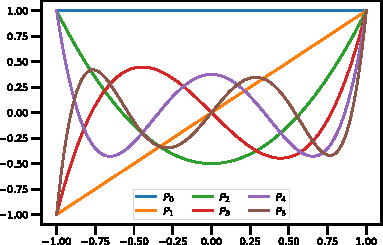
\includegraphics[scale=2.0]{legendre.pdf}
    }
    \caption{Первые шесть полиномов Лежандра.}\label{fig:pols}
\end{figure}

%
Полиномы Лежандра обладают следующими свойствами:
\begin{itemize}
    \item Ортогональность: набор многочленов Лежандра образует ортогональную систему, что означает:

    \begin{equation*}
        \int_{-1}^{1} L_m(x)L_n(x)dx = \frac{2}{2n+1}\delta_{mn}
    \end{equation*}
        
    \item Полнота: многочлены Лежандра являются полными. Это означает, что заданная кусочно-непрерывная функция $f(x)$ с конечным числом разрывов на интервале $[-1,1]$ может быть приближена следующей суммой:

    \begin{equation*}
        f_n(x) = \sum_{l=0}^{n} a_l L_l(x),
    \end{equation*}
    %
    где $a_l$ -- это коэффициент, $L_l(x)$ -- полином Лежандра степени $l$ и $f_n(x)~\rightarrow~f(x)$ при $n~\rightarrow~\infty$
    %
    Свойство полноты может быть записано в следующей форме:
    \begin{equation*}
        \sum_{l=0}^{\infty} \frac{2l+1}{2} L_l(x)L_l(y) = \delta(x-y).
    \end{equation*}
    При $x,y \in [-1,1]$ и $\delta(x-y)=\frac{1}{2\pi}\int_{-\infty}^{\infty} e^{ip(x-y)dp}$

    \item Рекуррентная формула Бонне: Многочлены Лежандра также могут быть определены как коэффициенты формального разложения в степенях $t$ производящей функции, описанной в работе Абрамовица [1974].
    \begin{equation*}
        \frac{1}{\sqrt{1-2xt+t^2}} = \sum_{n=0}^{\infty} L_n(x)t^n.
    \end{equation*}
    %
    Путем дифференцирования производящей функции по $t$ получается следующее:
    \begin{equation*}
        \frac{x-t}{\sqrt{1-2xt+t^2}} = (1-2xt+t^2)\sum_{n=1}^{\infty} nL_n(x)t^{n-1}.
    \end{equation*}
    
    Заменяя знаменатель левой части вышеприведенного уравнения суммой и перегруппировав всё уравнение, мы получаем:
    %
    \begin{equation*}
        nL_n(x)t^{n-1}-(2n+1)xL_n(x)t^n+(1+n)L_n(x)t^{n+1}=0.
    \end{equation*}
    
    Приравнивая коэффициенты при одинаковых степенях $t$, получаем:
    %
    \begin{equation*}
        (1+n)L_{1+n}(x)-(2n+1)xL_n(x)+nL_{n-1}(x) = 0, n \geq 2.
    \end{equation*}

    \item Другие свойства:
    \begin{equation*}
        \begin{aligned}
        & (2n+1)L_n(x)=L'_{n+1}(x) - L'_{n-1}(x), \\
        & L_n(-x) = (-1)^nL_n(x), \\
        & L_n(1) = 1, L_n(-1) = (-1)^n.
        \end{aligned}
    \end{equation*}

\end{itemize}

\subsubsection{Интерполяционные полиномы Лагранжа (узловой базис)}

% % \chapter{Оформление различных элементов}\label{ch:ch1}

% % \section{Форматирование текста}\label{sec:ch1/sec1}



% \section{Ссылки}\label{sec:ch1/sec2}

% Сошлёмся на библиографию.
% Одна ссылка: \cite[с.~54]{Sokolov}\cite[с.~36]{Gaidaenko}.
% Две ссылки: \cite{Sokolov,Gaidaenko}.
% Ссылка на собственные работы: \cite{vakbib1, confbib2}.
% Много ссылок: %\cite[с.~54]{Lermontov,Management,Borozda} % такой «фокус»
% %вызывает biblatex warning относительно опции sortcites, потому что неясно, к
% %какому источнику относится уточнение о страницах, а bibtex об этой проблеме
% %даже не предупреждает
% \cite{Lermontov, Management, Borozda, Marketing, Constitution, FamilyCode,
%     Gost.7.0.53, Razumovski, Lagkueva, Pokrovski, Methodology, Berestova,
%     Kriger}%
% \ifnumequal{\value{bibliosel}}{0}{% Примеры для bibtex8
%     \cite{Sirotko, Lukina, Encyclopedia, Nasirova}%
% }{% Примеры для biblatex через движок biber
%     \cite{Sirotko2, Lukina2, Encyclopedia2, Nasirova2}%
% }%
% .
% И~ещё немного ссылок:~\cite{Article,Book,Booklet,Conference,Inbook,Incollection,Manual,Mastersthesis,
%     Misc,Phdthesis,Proceedings,Techreport,Unpublished}
% % Следует обратить внимание, что пробел после запятой внутри \cite{}
% % обрабатывается ожидаемо, а пробел перед запятой, может вызывать проблемы при
% % обработке ссылок.
% \cite{medvedev2006jelektronnye, CEAT:CEAT581, doi:10.1080/01932691.2010.513279,
%     Gosele1999161,Li2007StressAnalysis, Shoji199895, test:eisner-sample,
%     test:eisner-sample-shorted, AB_patent_Pomerantz_1968, iofis_patent1960}%
% \ifnumequal{\value{bibliosel}}{0}{% Примеры для bibtex8
% }{% Примеры для biblatex через движок biber
%     \cite{patent2h, patent3h, patent2}%
% }%
% .

% \ifnumequal{\value{bibliosel}}{0}{% Примеры для bibtex8
% Попытка реализовать несколько ссылок на конкретные страницы
% для \texttt{bibtex} реализации библиографии:
% [\citenum{Sokolov}, с.~54; \citenum{Gaidaenko}, с.~36].
% }{% Примеры для biblatex через движок biber
% Несколько источников (мультицитата):
% % Тут специально написано по-разному тире, для демонстрации, что
% % применение специальных тире в настоящий момент в biblatex приводит к непоказу
% % "с.".
% \cites[vii--x, 5, 7]{Sokolov}[v"--~x, 25, 526]{Gaidaenko}[vii--x, 5, 7]{Techreport},
% работает только в \texttt{biblatex} реализации библиографии.
% }%

% Ссылки на собственные работы:~\cite{vakbib1, confbib1}.

% Сошлёмся на приложения: Приложение~\cref{app:A}, Приложение~\cref{app:B2}.

% Сошлёмся на формулу: формула~\cref{eq:equation1}.

% Сошлёмся на изображение: рисунок~\cref{fig:knuth}.

% Стандартной практикой является добавление к ссылкам префикса, характеризующего тип элемента.
% Это не является строгим требованием, но~позволяет лучше ориентироваться в документах большого размера.
% Например, для ссылок на~рисунки используется префикс \textit{fig},
% для ссылки на~таблицу "--- \textit{tab}.

% В таблице \cref{tab:tab_pref} приложения~\cref{app:B4} приведён список рекомендуемых
% к использованию стандартных префиксов.

% В некоторых ситуациях возникает необходимость отойти от требований ГОСТ по оформлению ссылок на
% литературу.
% В таком случае можно воспользоваться дополнительными опциями пакета \verb+biblatex+.

% Например, в ссылке на книгу~\cite{sobenin_kdv} использование опции \verb+maxnames=4+ позволяет
% вывести имена всех четырёх авторов.
% По ГОСТ имена последних трёх авторов опускаются.

% Кроме того, часто возникают проблемы с транслитерованными инициалами. Некоторые буквы русского
% алфавита по правилам транслитерации записываются двумя буквами латинского алфавита (ю-yu, ё-yo и
% т.д.).
% Такие инициалы \verb+biblatex+ будет сокращать до одной буквы, что неверно.
% Поправить его работу можно использовав опцию \verb+giveninits=false+.
% Пример использования этой опции можно видеть в ссылке~\cite{initials}.

% \section{Формулы}\label{sec:ch1/sec3}

% Благодаря пакету \textit{icomma}, \LaTeX~одинаково хорошо воспринимает
% в~качестве десятичного разделителя и запятую (\(3,1415\)), и точку (\(3.1415\)).

% \subsection{Ненумерованные одиночные формулы}\label{subsec:ch1/sec3/sub1}

% Вот так может выглядеть формула, которую необходимо вставить в~строку
% по~тексту: \(x \approx \sin x\) при \(x \to 0\).

% А вот так выглядит ненумерованная отдельностоящая формула c подстрочными
% и надстрочными индексами:
% \[
%     (x_1+x_2)^2 = x_1^2 + 2 x_1 x_2 + x_2^2
% \]

% Формула с неопределенным интегралом:
% \[
%     \int f(\alpha+x)=\sum\beta
% \]

% При использовании дробей формулы могут получаться очень высокие:
% \[
%     \frac{1}{\sqrt{2}+
%         \displaystyle\frac{1}{\sqrt{2}+
%             \displaystyle\frac{1}{\sqrt{2}+\cdots}}}
% \]

% В формулах можно использовать греческие буквы:
% %Все \original... команды заранее, ради этого примера, определены в Dissertation\userstyles.tex
% \[
%     \alpha\beta\gamma\delta\originalepsilon\epsilon\zeta\eta\theta%
%     \vartheta\iota\kappa\varkappa\lambda\mu\nu\xi\pi\varpi\rho\varrho%
%     \sigma\varsigma\tau\upsilon\originalphi\phi\chi\psi\omega\Gamma\Delta%
%     \Theta\Lambda\Xi\Pi\Sigma\Upsilon\Phi\Psi\Omega
% \]
% \[%https://texfaq.org/FAQ-boldgreek
%     \boldsymbol{\alpha\beta\gamma\delta\originalepsilon\epsilon\zeta\eta%
%         \theta\vartheta\iota\kappa\varkappa\lambda\mu\nu\xi\pi\varpi\rho%
%         \varrho\sigma\varsigma\tau\upsilon\originalphi\phi\chi\psi\omega\Gamma%
%         \Delta\Theta\Lambda\Xi\Pi\Sigma\Upsilon\Phi\Psi\Omega}
% \]

% Для добавления формул можно использовать пары \verb+$+\dots\verb+$+ и \verb+$$+\dots\verb+$$+,
% но~они считаются устаревшими.
% Лучше использовать их функциональные аналоги \verb+\(+\dots\verb+\)+ и \verb+\[+\dots\verb+\]+.

% \subsection{Ненумерованные многострочные формулы}\label{subsec:ch1/sec3/sub2}

% Вот так можно написать две формулы, не нумеруя их, чтобы знаки <<равно>> были
% строго друг под другом:
% \begin{align}
%     f_W & =  \min \left( 1, \max \left( 0, \frac{W_{soil} / W_{max}}{W_{crit}} \right)  \right), \nonumber \\
%     f_T & =  \min \left( 1, \max \left( 0, \frac{T_s / T_{melt}}{T_{crit}} \right)  \right), \nonumber
% \end{align}

% Выровнять систему ещё и по переменной \( x \) можно, используя окружение
% \verb|alignedat| из пакета \verb|amsmath|. Вот так:
% \[
% |x| = \left\{
% \begin{alignedat}{2}
%     &&x, \quad &\text{eсли } x\geqslant 0 \\
%     &-&x, \quad & \text{eсли } x<0
% \end{alignedat}
% \right.
% \]
% Здесь первый амперсанд (в исходном \LaTeX\ описании формулы) означает
% выравнивание по~левому краю, второй "--- по~\( x \), а~третий "--- по~слову
% <<если>>. Команда \verb|\quad| делает большой горизонтальный пробел.

% Ещё вариант:
% \[
%     |x|=
%     \begin{cases}
%         \phantom{-}x, \text{если } x \geqslant 0 \\
%         -x, \text{если } x<0
%     \end{cases}
% \]

% Кроме того, для  нумерованных формул \verb|alignedat| делает вертикальное
% выравнивание номера формулы по центру формулы. Например, выравнивание
% компонент вектора:
% \begin{equation}
%     \label{eq:2p3}
%     \begin{alignedat}{2}
%         {\mathbf{N}}_{o1n}^{(j)} = \,{\sin} \phi\,n\!\left(n+1\right)
%         {\sin}\theta\,
%         \pi_n\!\left({\cos} \theta\right)
%         \frac{
%         z_n^{(j)}\!\left( \rho \right)
%         }{\rho}\,
%         &{\boldsymbol{\hat{\mathrm e}}}_{r}\,+   \\
%         +\,
%         {\sin} \phi\,
%         \tau_n\!\left({\cos} \theta\right)
%         \frac{
%         \left[\rho z_n^{(j)}\!\left( \rho \right)\right]^{\prime}
%         }{\rho}\,
%         &{\boldsymbol{\hat{\mathrm e}}}_{\theta}\,+   \\
%         +\,
%         {\cos} \phi\,
%         \pi_n\!\left({\cos} \theta\right)
%         \frac{
%         \left[\rho z_n^{(j)}\!\left( \rho \right)\right]^{\prime}
%         }{\rho}\,
%         &{\boldsymbol{\hat{\mathrm e}}}_{\phi}\:.
%     \end{alignedat}
% \end{equation}

% Ещё об отступах. Иногда для лучшей <<читаемости>> формул полезно
% немного исправить стандартные интервалы \LaTeX\ с учётом логической
% структуры самой формулы. Например в формуле~\cref{eq:2p3} добавлен
% небольшой отступ \verb+\,+ между основными сомножителями, ниже
% результат применения всех вариантов отступа:
% \begin{align*}
%     \backslash!             & \quad f(x) = x^2\! +3x\! +2         \\
%     \mbox{по-умолчанию}     & \quad f(x) = x^2+3x+2               \\
%     \backslash,             & \quad f(x) = x^2\, +3x\, +2         \\
%     \backslash{:}           & \quad f(x) = x^2\: +3x\: +2         \\
%     \backslash;             & \quad f(x) = x^2\; +3x\; +2         \\
%     \backslash \mbox{space} & \quad f(x) = x^2\ +3x\ +2           \\
%     \backslash \mbox{quad}  & \quad f(x) = x^2\quad +3x\quad +2   \\
%     \backslash \mbox{qquad} & \quad f(x) = x^2\qquad +3x\qquad +2
% \end{align*}

% Можно использовать разные математические алфавиты:
% \begin{align}
%     \mathcal{ABCDEFGHIJKLMNOPQRSTUVWXYZ} \nonumber  \\
%     \mathfrak{ABCDEFGHIJKLMNOPQRSTUVWXYZ} \nonumber \\
%     \mathbb{ABCDEFGHIJKLMNOPQRSTUVWXYZ} \nonumber
% \end{align}

% Посмотрим на систему уравнений на примере аттрактора Лоренца:

% \[
% \left\{
% \begin{array}{rl}
%     \dot x = & \sigma (y-x)  \\
%     \dot y = & x (r - z) - y \\
%     \dot z = & xy - bz
% \end{array}
% \right.
% \]

% А для вёрстки матриц удобно использовать многоточия:
% \[
%     \left(
%         \begin{array}{ccc}
%             a_{11} & \ldots & a_{1n} \\
%             \vdots & \ddots & \vdots \\
%             a_{n1} & \ldots & a_{nn} \\
%         \end{array}
%     \right)
% \]

% \subsection{Нумерованные формулы}\label{subsec:ch1/sec3/sub3}

% А вот так пишется нумерованная формула:
% \begin{equation}
%     \label{eq:equation1}
%     e = \lim_{n \to \infty} \left( 1+\frac{1}{n} \right) ^n
% \end{equation}

% Нумерованных формул может быть несколько:
% \begin{equation}
%     \label{eq:equation2}
%     \lim_{n \to \infty} \sum_{k=1}^n \frac{1}{k^2} = \frac{\pi^2}{6}
% \end{equation}

% Впоследствии на формулы~\cref{eq:equation1, eq:equation2} можно ссылаться.

% Сделать так, чтобы номер формулы стоял напротив средней строки, можно,
% используя окружение \verb|multlined| (пакет \verb|mathtools|) вместо
% \verb|multline| внутри окружения \verb|equation|. Вот так:
% \begin{equation} % \tag{S} % tag - вписывает свой текст
%     \label{eq:equation3}
%     \begin{multlined}
%         1+ 2+3+4+5+6+7+\dots + \\
%         + 50+51+52+53+54+55+56+57 + \dots + \\
%         + 96+97+98+99+100=5050
%     \end{multlined}
% \end{equation}

% Уравнения~\cref{eq:subeq_1,eq:subeq_2} демонстрируют возможности
% окружения \verb|\subequations|.
% \begin{subequations}
%     \label{eq:subeq_1}
%     \begin{gather}
%         y = x^2 + 1 \label{eq:subeq_1-1} \\
%         y = 2 x^2 - x + 1 \label{eq:subeq_1-2}
%     \end{gather}
% \end{subequations}
% Ссылки на отдельные уравнения~\cref{eq:subeq_1-1,eq:subeq_1-2,eq:subeq_2-1}.
% \begin{subequations}
%     \label{eq:subeq_2}
%     \begin{align}
%         y & = x^3 + x^2 + x + 1 \label{eq:subeq_2-1} \\
%         y & = x^2
%     \end{align}
% \end{subequations}

% \subsection{Форматирование чисел и размерностей величин}\label{sec:units}

% Числа форматируются при помощи команды \verb|\num|:
% \num{5,3};
% \num{2,3e8};
% \num{12345,67890};
% \num{2,6 d4};
% \num{1+-2i};
% \num{.3e45};
% \num[exponent-base=2]{5 e64};
% \num[exponent-base=2,exponent-to-prefix]{5 e64};
% \num{1.654 x 2.34 x 3.430}
% \num{1 2 x 3 / 4}.
% Для написания последовательности чисел можно использовать команды \verb|\numlist| и \verb|\numrange|:
% \numlist{10;30;50;70}; \numrange{10}{30}.
% Значения углов можно форматировать при помощи команды \verb|\ang|:
% \ang{2.67};
% \ang{30,3};
% \ang{-1;;};
% \ang{;-2;};
% \ang{;;-3};
% \ang{300;10;1}.

% Обратите внимание, что ГОСТ запрещает использование знака <<->> для обозначения отрицательных чисел
% за исключением формул, таблиц и~рисунков.
% Вместо него следует использовать слово <<минус>>.

% Размерности можно записывать при помощи команд \verb|\si| и \verb|\SI|:
% \si{\farad\squared\lumen\candela};
% \si{\joule\per\mole\per\kelvin};
% \si[per-mode = symbol-or-fraction]{\joule\per\mole\per\kelvin};
% \si{\metre\per\second\squared};
% \SI{0.10(5)}{\neper};
% \SI{1.2-3i e5}{\joule\per\mole\per\kelvin};
% \SIlist{1;2;3;4}{\tesla};
% \SIrange{50}{100}{\volt}.
% Список единиц измерений приведён в таблицах~\cref{tab:unit:base,
%     tab:unit:derived,tab:unit:accepted,tab:unit:physical,tab:unit:other}.
% Приставки единиц приведены в~таблице~\cref{tab:unit:prefix}.

% С дополнительными опциями форматирования можно ознакомиться в~описании пакета \texttt{siunitx};
% изменить или добавить единицы измерений можно в~файле \texttt{siunitx.cfg}.

% \begin{table}
%     \centering
%     \captionsetup{justification=centering} % выравнивание подписи по-центру
%     \caption{Основные величины СИ}\label{tab:unit:base}
%     \begin{tabular}{llc}
%         \toprule
%         Название  & Команда                 & Символ         \\
%         \midrule
%         Ампер     & \verb|\ampere| & \si{\ampere}   \\
%         Кандела   & \verb|\candela| & \si{\candela}  \\
%         Кельвин   & \verb|\kelvin| & \si{\kelvin}   \\
%         Килограмм & \verb|\kilogram| & \si{\kilogram} \\
%         Метр      & \verb|\metre| & \si{\metre}    \\
%         Моль      & \verb|\mole| & \si{\mole}     \\
%         Секунда   & \verb|\second| & \si{\second}   \\
%         \bottomrule
%     \end{tabular}
% \end{table}

% \begin{table}
%     \small
%     \centering
%     \begin{threeparttable}% выравнивание подписи по границам таблицы
%         \caption{Производные единицы СИ}\label{tab:unit:derived}
%         \begin{tabular}{llc|llc}
%             \toprule
%             Название       & Команда                 & Символ              & Название & Команда & Символ \\
%             \midrule
%             Беккерель      & \verb|\becquerel| & \si{\becquerel}     &
%             Ньютон         & \verb|\newton| & \si{\newton}                                      \\
%             Градус Цельсия & \verb|\degreeCelsius| & \si{\degreeCelsius} &
%             Ом             & \verb|\ohm| & \si{\ohm}                                         \\
%             Кулон          & \verb|\coulomb| & \si{\coulomb}       &
%             Паскаль        & \verb|\pascal| & \si{\pascal}                                      \\
%             Фарад          & \verb|\farad| & \si{\farad}         &
%             Радиан         & \verb|\radian| & \si{\radian}                                      \\
%             Грей           & \verb|\gray| & \si{\gray}          &
%             Сименс         & \verb|\siemens| & \si{\siemens}                                     \\
%             Герц           & \verb|\hertz| & \si{\hertz}         &
%             Зиверт         & \verb|\sievert| & \si{\sievert}                                     \\
%             Генри          & \verb|\henry| & \si{\henry}         &
%             Стерадиан      & \verb|\steradian| & \si{\steradian}                                   \\
%             Джоуль         & \verb|\joule| & \si{\joule}         &
%             Тесла          & \verb|\tesla| & \si{\tesla}                                       \\
%             Катал          & \verb|\katal| & \si{\katal}         &
%             Вольт          & \verb|\volt| & \si{\volt}                                        \\
%             Люмен          & \verb|\lumen| & \si{\lumen}         &
%             Ватт           & \verb|\watt| & \si{\watt}                                        \\
%             Люкс           & \verb|\lux| & \si{\lux}           &
%             Вебер          & \verb|\weber| & \si{\weber}                                       \\
%             \bottomrule
%         \end{tabular}
%     \end{threeparttable}
% \end{table}

% \begin{table}
%     \centering
%     \begin{threeparttable}% выравнивание подписи по границам таблицы
%         \caption{Внесистемные единицы}\label{tab:unit:accepted}

%         \begin{tabular}{llc}
%             \toprule
%             Название        & Команда                 & Символ          \\
%             \midrule
%             День            & \verb|\day| & \si{\day}       \\
%             Градус          & \verb|\degree| & \si{\degree}    \\
%             Гектар          & \verb|\hectare| & \si{\hectare}   \\
%             Час             & \verb|\hour| & \si{\hour}      \\
%             Литр            & \verb|\litre| & \si{\litre}     \\
%             Угловая минута  & \verb|\arcminute| & \si{\arcminute} \\
%             Угловая секунда & \verb|\arcsecond| & \si{\arcsecond} \\ %
%             Минута          & \verb|\minute| & \si{\minute}    \\
%             Тонна           & \verb|\tonne| & \si{\tonne}     \\
%             \bottomrule
%         \end{tabular}
%     \end{threeparttable}
% \end{table}

% \begin{table}
%     \centering
%     \captionsetup{justification=centering}
%     \caption{Внесистемные единицы, получаемые из эксперимента}\label{tab:unit:physical}
%     \begin{tabular}{llc}
%         \toprule
%         Название                & Команда                 & Символ                 \\
%         \midrule
%         Астрономическая единица & \verb|\astronomicalunit| & \si{\astronomicalunit} \\
%         Атомная единица массы   & \verb|\atomicmassunit| & \si{\atomicmassunit}   \\
%         Боровский радиус        & \verb|\bohr| & \si{\bohr}             \\
%         Скорость света          & \verb|\clight| & \si{\clight}           \\
%         Дальтон                 & \verb|\dalton| & \si{\dalton}           \\
%         Масса электрона         & \verb|\electronmass| & \si{\electronmass}     \\
%         Электрон Вольт          & \verb|\electronvolt| & \si{\electronvolt}     \\
%         Элементарный заряд      & \verb|\elementarycharge| & \si{\elementarycharge} \\
%         Энергия Хартри          & \verb|\hartree| & \si{\hartree}          \\
%         Постоянная Планка       & \verb|\planckbar| & \si{\planckbar}        \\
%         \bottomrule
%     \end{tabular}
% \end{table}

% \begin{table}
%     \centering
%     \begin{threeparttable}% выравнивание подписи по границам таблицы
%         \caption{Другие внесистемные единицы}\label{tab:unit:other}
%         \begin{tabular}{llc}
%             \toprule
%             Название                  & Команда                 & Символ             \\
%             \midrule
%             Ангстрем                  & \verb|\angstrom| & \si{\angstrom}     \\
%             Бар                       & \verb|\bar| & \si{\bar}          \\
%             Барн                      & \verb|\barn| & \si{\barn}         \\
%             Бел                       & \verb|\bel| & \si{\bel}          \\
%             Децибел                   & \verb|\decibel| & \si{\decibel}      \\
%             Узел                      & \verb|\knot| & \si{\knot}         \\
%             Миллиметр ртутного столба & \verb|\mmHg| & \si{\mmHg}         \\
%             Морская миля              & \verb|\nauticalmile| & \si{\nauticalmile} \\
%             Непер                     & \verb|\neper| & \si{\neper}        \\
%             \bottomrule
%         \end{tabular}
%     \end{threeparttable}
% \end{table}

% \begin{table}
%     \small
%     \centering
%     \begin{threeparttable}% выравнивание подписи по границам таблицы
%         \caption{Приставки СИ}\label{tab:unit:prefix}
%         \begin{tabular}{llcc|llcc}
%             \toprule
%             Приставка & Команда                  & Символ      & Степень &
%             Приставка & Команда                  & Символ      & Степень   \\
%             \midrule
%             Иокто     & \verb|\yocto|  & \si{\yocto} & -24     &
%             Дека      & \verb|\deca|  & \si{\deca}  & 1         \\
%             Зепто     & \verb|\zepto|  & \si{\zepto} & -21     &
%             Гекто     & \verb|\hecto|  & \si{\hecto} & 2         \\
%             Атто      & \verb|\atto|  & \si{\atto}  & -18     &
%             Кило      & \verb|\kilo|  & \si{\kilo}  & 3         \\
%             Фемто     & \verb|\femto|  & \si{\femto} & -15     &
%             Мега      & \verb|\mega|  & \si{\mega}  & 6         \\
%             Пико      & \verb|\pico|  & \si{\pico}  & -12     &
%             Гига      & \verb|\giga|  & \si{\giga}  & 9         \\
%             Нано      & \verb|\nano|  & \si{\nano}  & -9      &
%             Терра     & \verb|\tera|  & \si{\tera}  & 12        \\
%             Микро     & \verb|\micro|  & \si{\micro} & -6      &
%             Пета      & \verb|\peta|  & \si{\peta}  & 15        \\
%             Милли     & \verb|\milli|  & \si{\milli} & -3      &
%             Екса      & \verb|\exa|  & \si{\exa}   & 18        \\
%             Санти     & \verb|\centi|  & \si{\centi} & -2      &
%             Зетта     & \verb|\zetta|  & \si{\zetta} & 21        \\
%             Деци      & \verb|\deci| & \si{\deci}  & -1      &
%             Иотта     & \verb|\yotta| & \si{\yotta} & 24        \\
%             \bottomrule
%         \end{tabular}
%     \end{threeparttable}
% \end{table}

% \subsection{Заголовки с формулами: \texorpdfstring{\(a^2 + b^2 = c^2\)}{%
%         a\texttwosuperior\ + b\texttwosuperior\ = c\texttwosuperior},
%     \texorpdfstring{\(\left\vert\textrm{{Im}}\Sigma\left(
%             \protect\varepsilon\right)\right\vert\approx const\)}{|ImΣ (ε)| ≈ const},
%     \texorpdfstring{\(\sigma_{xx}^{(1)}\)}{σ\_\{xx\}\textasciicircum\{(1)\}}
% }\label{subsec:with_math}

% Пакет \texttt{hyperref} берёт текст для закладок в pdf-файле из~аргументов
% команд типа \verb|\section|, которые могут содержать математические формулы,
% а~также изменения цвета текста или шрифта, которые не отображаются в~закладках.
% Чтобы использование формул в заголовках не вызывало в~логе компиляции появление
% предупреждений типа <<\texttt{Token not allowed in~a~PDF string
%     (Unicode):(hyperref) removing...}>>, следует использовать конструкцию
% \verb|\texorpdfstring{}{}|, где в~первых фигурных скобках указывается
% формула, а~во~вторых "--- запись формулы для закладок.

% \section{Рецензирование текста}\label{sec:markup}

% В шаблоне для диссертации и автореферата заданы команды рецензирования.
% Они видны при компиляции шаблона в режиме черновика или при установке
% соответствующей настройки (\verb+showmarkup+) в~файле \verb+common/setup.tex+.

% Команда \verb+\todo+ отмечает текст красным цветом.
% \todo{Например, так.}

% Команда \verb+\note+ позволяет выбрать цвет текста.
% \note{Чёрный, } \note[red]{красный, } \note[green]{зелёный, }
% \note[blue]{синий.} \note[orange]{Обратите внимание на ширину и расстановку
%     формирующихся пробелов, в~результате приведённой записи (зависит также
%     от~применяемого компилятора).}

% Окружение \verb+commentbox+ также позволяет выбрать цвет.

% \begin{commentbox}[red]
%     Красный текст.

%     Несколько параграфов красного текста.
% \end{commentbox}

% \begin{commentbox}[blue]
%     Синяя формула.

%     \begin{equation}
%         \alpha + \beta = \gamma
%     \end{equation}
% \end{commentbox}

% \verb+commentbox+ позволяет закомментировать участок кода в~режиме чистовика.
% Чтобы убрать кусок кода для всех режимов, можно использовать окружение
% \verb+comment+.

% \begin{comment}
% Этот текст всегда скрыт.
% \end{comment}

% \section{Работа со списком сокращений и~условных обозначений}\label{sec:acronyms}

% С помощью пакета \texttt{nomencl} можно создавать удобный сортированный список
% сокращений и условных обозначений во время написания текста. Вызов
% \verb+\nomenclature+ добавляет нужный символ или сокращение с~описанием
% в~список, который затем печатается вызовом \verb+\printnomenclature+
% в~соответствующем разделе.
% Для того, чтобы эти операции прошли, потребуется дополнительный вызов
% \verb+makeindex -s nomencl.ist -o %.nls %.nlo+ в~командной строке, где вместо
% \verb+%+ следует подставить имя главного файла проекта (\verb+dissertation+
% для этого шаблона).
% Затем потребуется один или два дополнительных вызова компилятора проекта.
% \begin{equation}
%     \omega = c k,
% \end{equation}
% где \( \omega \) "--- частота света, \( c \) "--- скорость света, \( k \) "---
% модуль волнового вектора.
% \nomenclature{\(\omega\)}{частота света\nomrefeq}
% \nomenclature{\(c\)}{скорость света\nomrefpage}
% \nomenclature{\(k\)}{модуль волнового вектора\nomrefeqpage}
% Использование
% \begin{verbatim}
% \nomenclature{\(\omega\)}{частота света\nomrefeq}
% \nomenclature{\(c\)}{скорость света\nomrefpage}
% \nomenclature{\(k\)}{модуль волнового вектора\nomrefeqpage}
% \end{verbatim}
% после уравнения добавит в список условных обозначений три записи.
% Ссылки \verb+\nomrefeq+ на последнее уравнение, \verb+\nomrefpage+ "--- на
% страницу, \verb+\nomrefeqpage+ "--- сразу на~последнее уравнение и~на~страницу,
% можно опускать и~не~использовать.

% Группировкой и сортировкой пунктов в списке можно управлять с~помощью указания
% дополнительных аргументов к команде \verb+nomenclature+.
% Например, при вызове
% \begin{verbatim}
% \nomenclature[03]{\( \hbar \)}{постоянная Планка}
% \nomenclature[01]{\( G \)}{гравитационная постоянная}
% \end{verbatim}
% \( G \) будет стоять в списке выше, чем \( \hbar \).
% Для корректных вертикальных отступов между строками в описании лучше
% не~использовать многострочные формулы в~списке обозначений.

% \nomenclature{%
%     \( \begin{rcases}
%         a_n \\
%         b_n
%     \end{rcases} \)%
% }{коэффициенты разложения Ми в дальнем поле соответствующие электрическим и
%     магнитным мультиполям}
% \nomenclature[a\( e \)]{\( {\boldsymbol{\hat{\mathrm e}}} \)}{единичный вектор}
% \nomenclature{\( E_0 \)}{амплитуда падающего поля}
% \nomenclature{\( j \)}{тип функции Бесселя}
% \nomenclature{\( k \)}{волновой вектор падающей волны}
% \nomenclature{%
%     \( \begin{rcases}
%         a_n \\
%         b_n
%     \end{rcases} \)%
% }{и снова коэффициенты разложения Ми в дальнем поле соответствующие
%     электрическим и магнитным мультиполям. Добавлено много текста, так что
%     описание группы условных обозначений значительно превысило высоту этой
%     группы...}
% \nomenclature{\( L \)}{общее число слоёв}
% \nomenclature{\( l \)}{номер слоя внутри стратифицированной сферы}
% \nomenclature{\( \lambda \)}{длина волны электромагнитного излучения в вакууме}
% \nomenclature{\( n \)}{порядок мультиполя}
% \nomenclature{%
%     \( \begin{rcases}
%         {\mathbf{N}}_{e1n}^{(j)} & {\mathbf{N}}_{o1n}^{(j)} \\
%         {\mathbf{M}_{o1n}^{(j)}} & {\mathbf{M}_{e1n}^{(j)}}
%     \end{rcases} \)%
% }{сферические векторные гармоники}
% \nomenclature{\( \mu \)}{магнитная проницаемость в вакууме}
% \nomenclature{\( r, \theta, \phi \)}{полярные координаты}
% \nomenclature{\( \omega \)}{частота падающей волны}

% С помощью \verb+nomenclature+ можно включать в~список сокращения,
% не~используя их~в~тексте.
% % запись сокращения в список происходит командой \nomenclature,
% % а не употреблением самого сокращения
% \nomenclature{FEM}{finite element method, метод конечных элементов}
% \nomenclature{FIT}{finite integration technique, метод конечных интегралов}
% \nomenclature{FMM}{fast multipole method, быстрый метод многополюсника}
% \nomenclature{FVTD}{finite volume time-domain, метод конечных объёмов
%     во~временной области}
% \nomenclature{MLFMA}{multilevel fast multipole algorithm, многоуровневый
%     быстрый алгоритм многополюсника}
% \nomenclature{BEM}{boundary element method, метод граничных элементов}
% \nomenclature{CST MWS}{Computer Simulation Technology Microwave Studio
%     программа для компьютерного моделирования уравнен Максвелла}
% \nomenclature{DDA}{discrete dipole approximation, приближение дискретиных
%     диполей}
% \nomenclature{FDFD}{finite difference frequency domain, метод конечных
%     разностей в~частотной области}
% \nomenclature{FDTD}{finite difference time domain, метод конечных разностей
%     во~временной области}
% \nomenclature{MoM}{method of moments, метод моментов}
% \nomenclature{MSTM}{multiple sphere T-Matrix, метод Т-матриц для множества
%     сфер}
% \nomenclature{PSTD}{pseudospectral time domain method, псевдоспектральный метод
%     во~временной области}
% \nomenclature{TLM}{transmission line matrix method, метод матриц линий передач}

\FloatBarrier
           % Глава 1
\chapter{Обратное течение в квадратном канале}\label{ch:ch2}
\section{Постановка задачи}\label{sec:ch2/problem}
%
В работе рассматривается перенос температуры как в приближении пассивной примеси, 
так и в приближении малого числа Маха в канале квадратного поперечного сечения шириной $2H$. 
%
Геометория задачи показана на Рисунке \ref{fig:geom}
%
В качестве теплоносителя рассматривался свинцово-висмутовый сплав.
% 
Был выбран диапазон температур от $373^\circ K$ до $573^\circ K$. 
%
Ниже, на Рисунке \ref{fig:cond}-\ref{fig:pr} представлены зависимости основных параметров от температуры, 
обезразмеренные соответствующим образом, а также их аппроксимация полиномами.
%
\begin{figure}[ht]
    \centerfloat{
        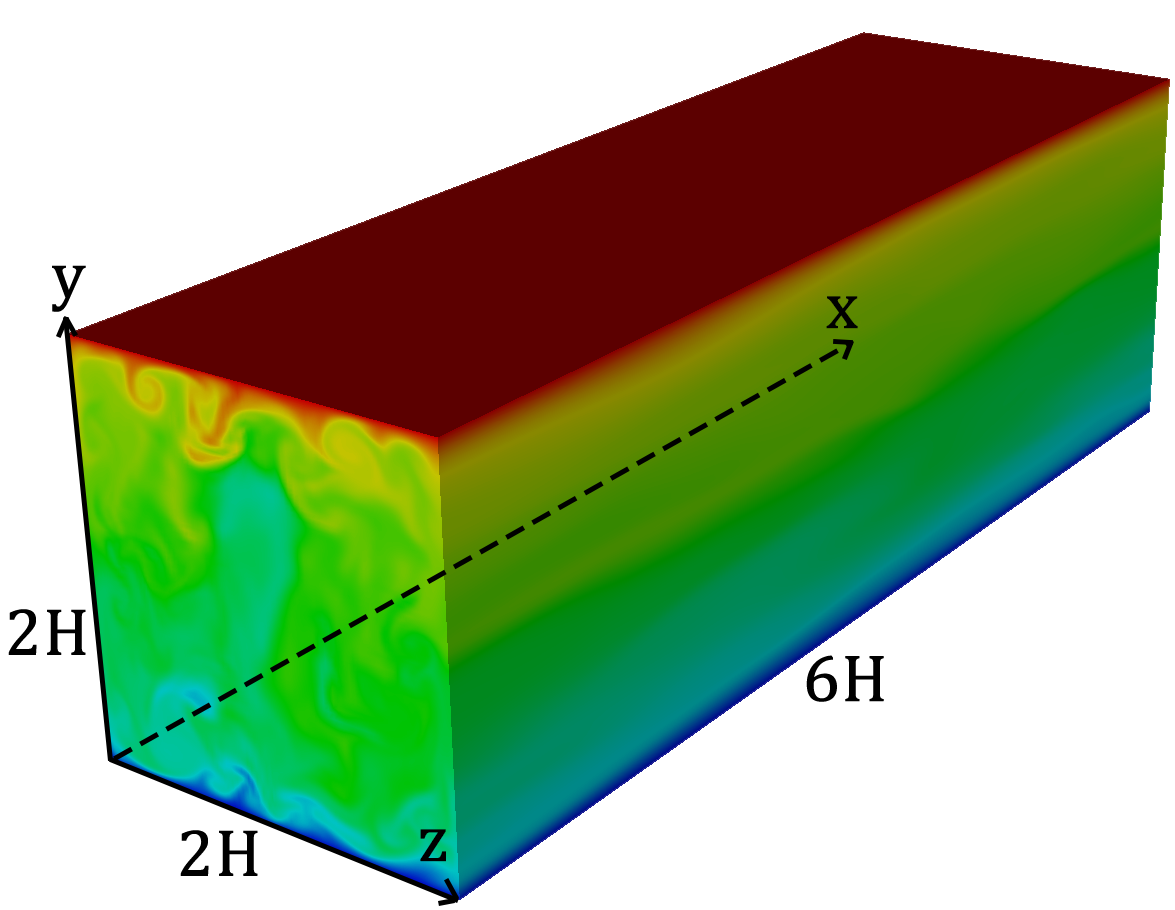
\includegraphics[scale=0.3]{Geometry1.png}
    }
    \caption{Геометрия задачи, где $x\in[0,6]$, $y\in[-1,1]$, $z\in[-1,1]$}\label{fig:geom}
\end{figure}
\begin{figure}[ht]
    \centerfloat{
        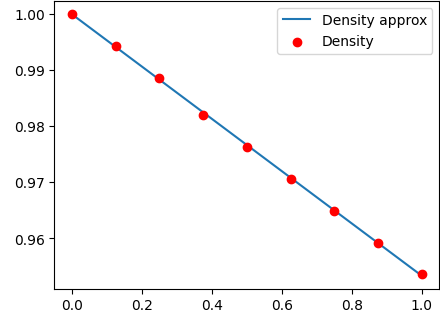
\includegraphics[scale=1.0]{Density.png}
    }
    \caption{Зависимость плотности от температуры}\label{fig:cond}
\end{figure}
\begin{figure}[ht]
    \centerfloat{
        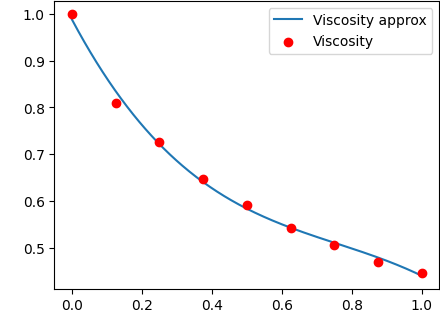
\includegraphics[scale=1.0]{Viscosity.png}
    }
    \caption{Зависимость кинематической вязкости от температуры}\label{fig:visc}
\end{figure}
\begin{figure}[ht]
    \centerfloat{
        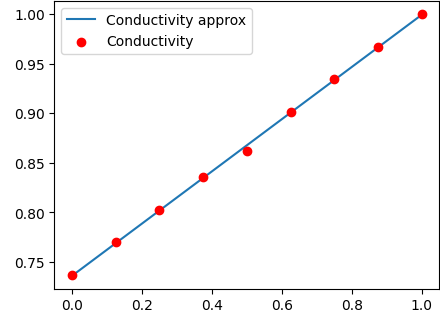
\includegraphics[scale=1.0]{Conductivity.png}
    }
    \caption{Зависимость коэффициента теплопроводности от температуры}\label{fig:cp}
\end{figure}
\begin{figure}[ht]
    \centerfloat{
        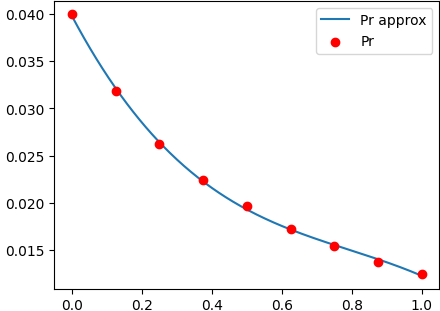
\includegraphics[scale=1.0]{Pr.png}
    }
    \caption{Зависимость числа Прандтля от температуры}\label{fig:pr}
\end{figure}

%
Для решения уравнения Навье-Стокса вплоть до колмогровского масштаба вблизи стенок используется сгущение сетки. 
%
Всего в сетке содержится $18\times32\times32$ спектральных элементов, 
в качестве базисных функций выступают полиномы Лагранжа 8 порядка. 
%
Благодаря спектральной точности кода удается добиться хорошей точности решения 
на относительно небольшом количестве вычислительных узлов, которое для данной задачи не превысило 10 млн. 
%

Для скорости используются периодические граничные условия в продольном направлении и условие прилипания 
на боковых стенках канала, для температуры формулируется задача Дирихле 
на верхней и нижней стенках  $(y/H=\pm1)$, боковые стенки теплоизолированы. 
%
Число Рейнольдса равно $Re = 3150$, построенное по среднерасходной скорости и полувысоте канала. 
%
Зависимости плотности и вязкости от температуры выбраны в соответствии с табличными данными 
и оберазмеренными соответствующим образом.
%

\section{Результаты}\label{sec:ch2/results}
%
%
\begin{figure}[ht]
    \centerfloat{
        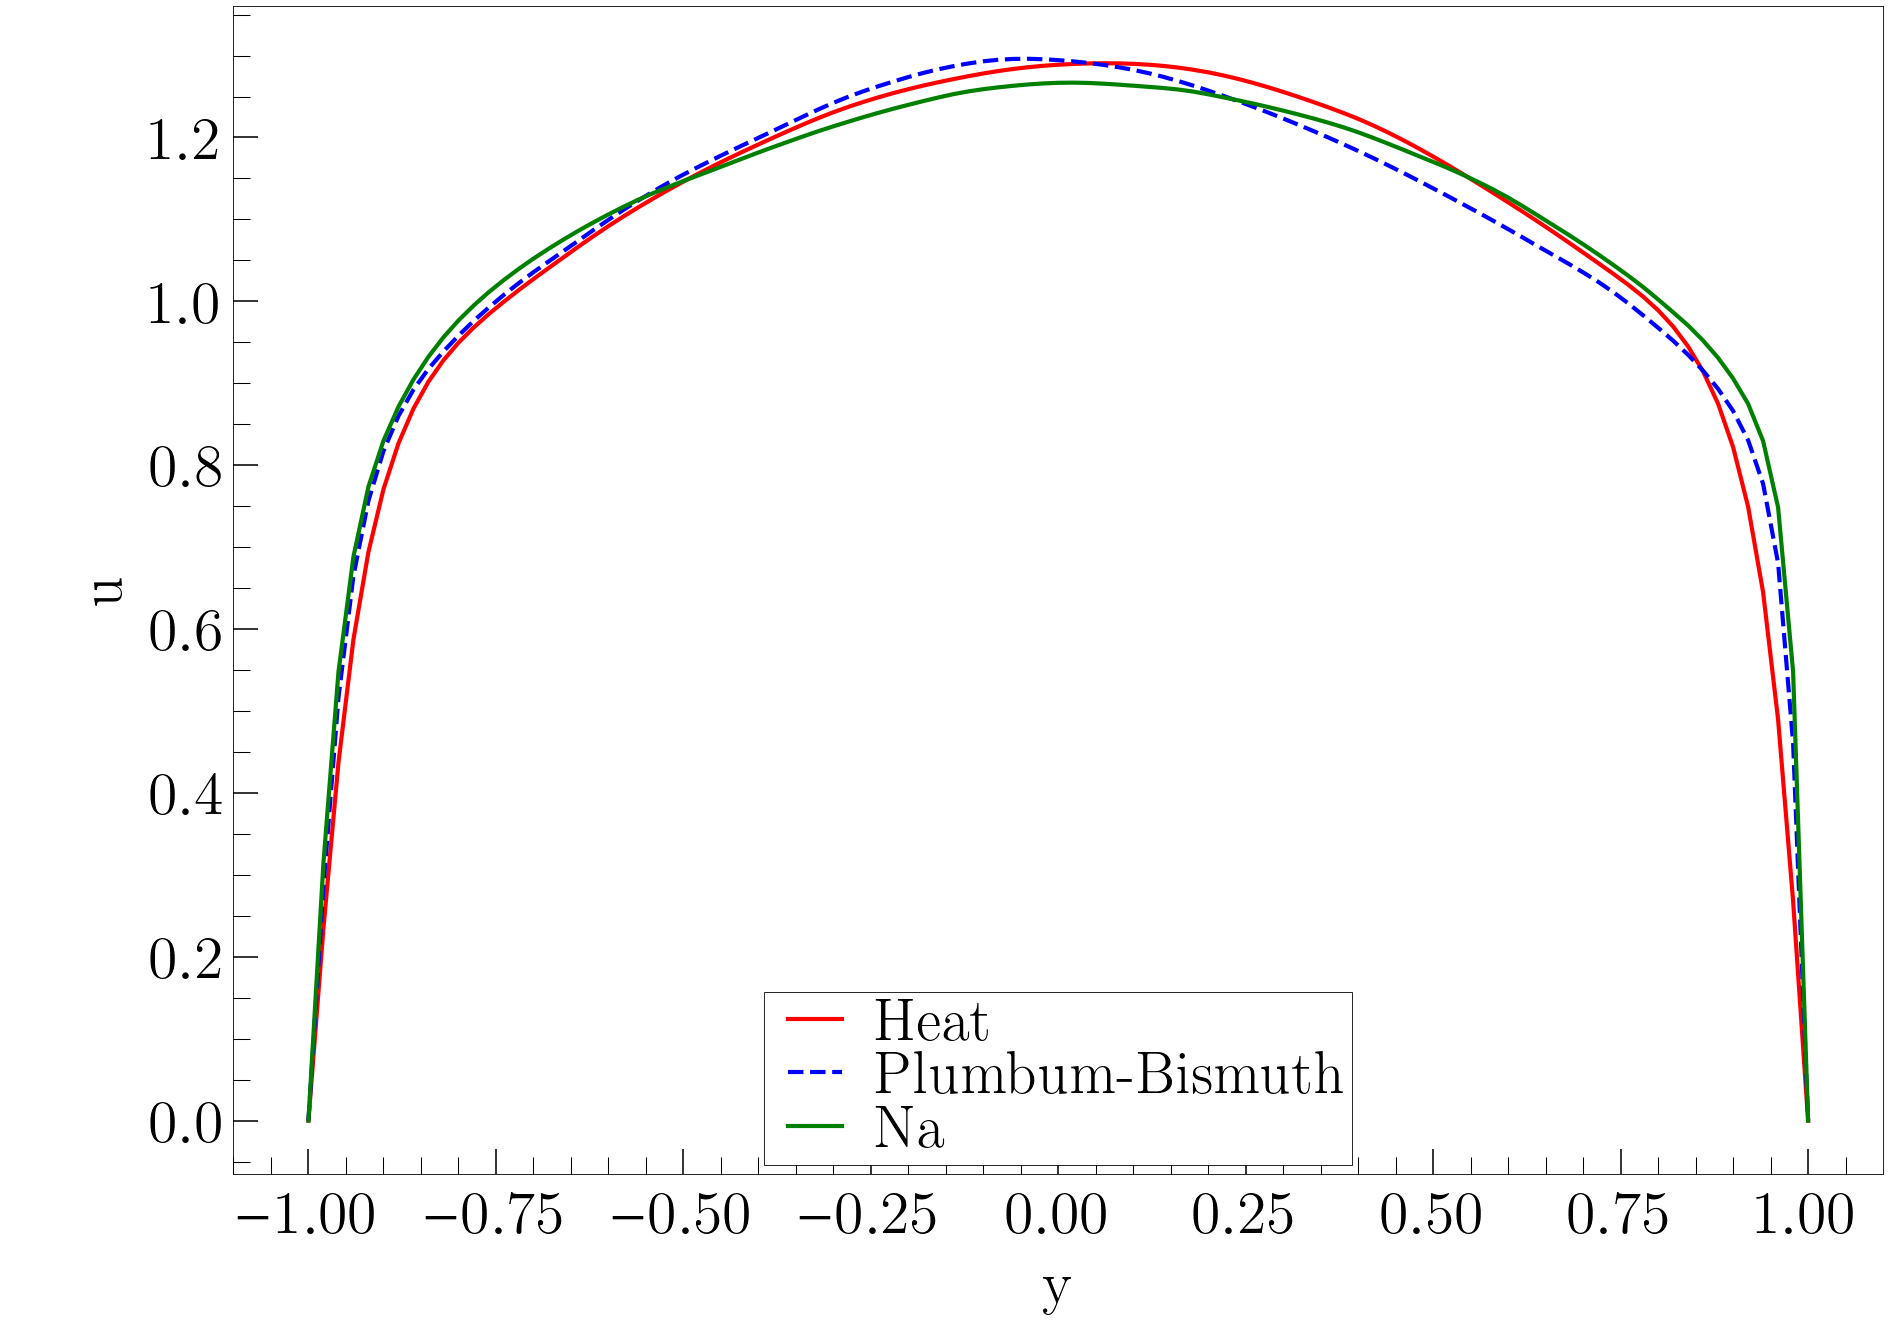
\includegraphics[scale=0.7]{u.png}
    }
    \caption{Осредненное поле продольной скорости в точке $z=0$, где Heat – пассивная примесь, Plumbum-Bismuth – режим малого числа Маха для свинцово - висмутного сплава, Na - аналогичный расчет для жидкого натрия}\label{fig:u}
\end{figure}
%
%
\begin{figure}[ht]
    \centerfloat{
        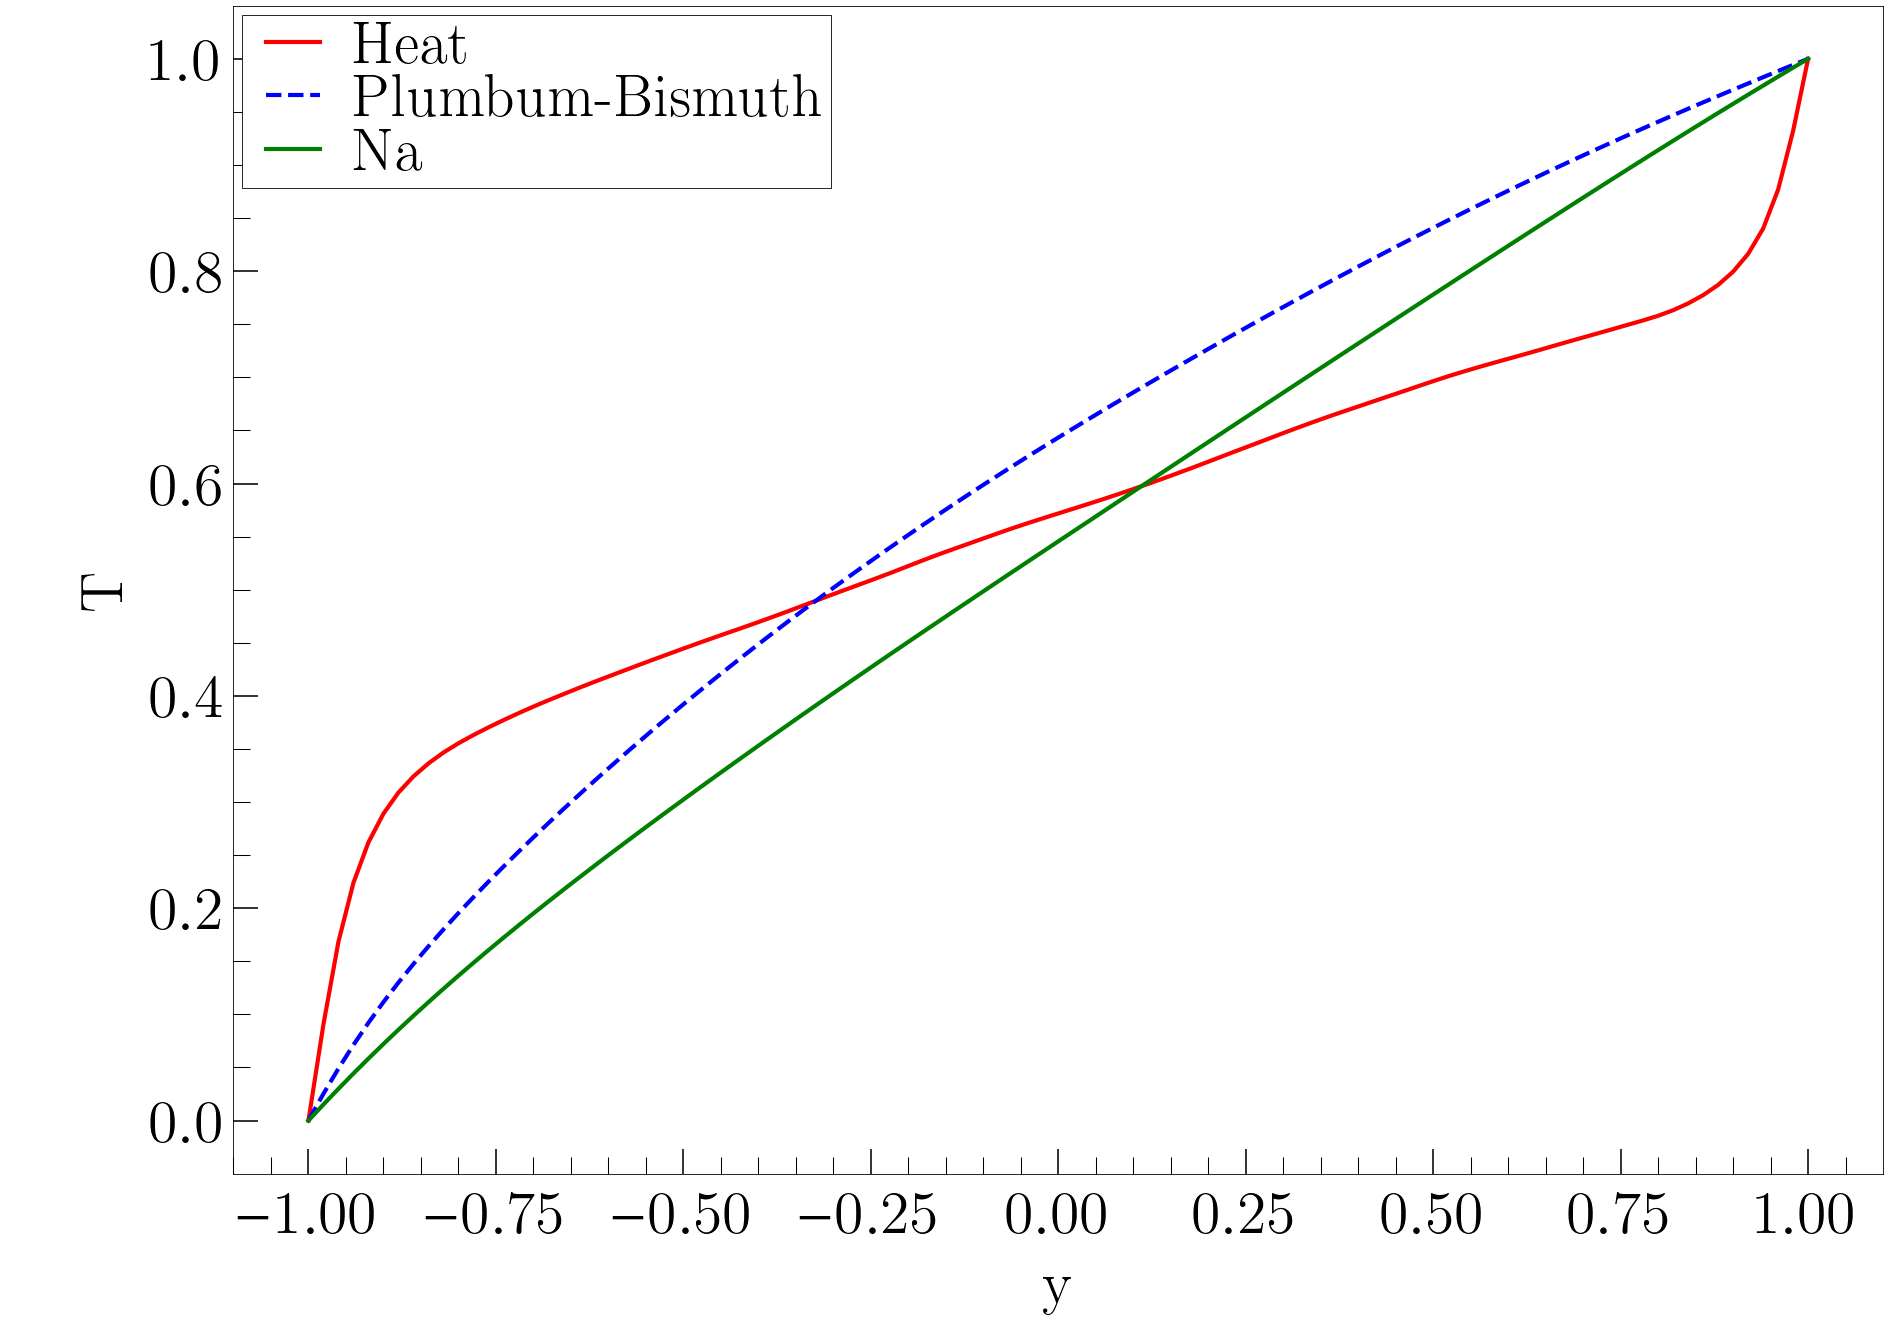
\includegraphics[scale=0.7]{T.png}
    }
    \caption{Поле температуры в точке $z=0$ в начальный момент времени, где Heat – пассивная примесь, Plumbum-Bismuth – режим малого числа Маха для свинцово - висмутного сплава, Na - аналогичный расчет для жидкого натрия}\label{fig:T}
\end{figure}


Был проведен анализ профилей средней скорости и температуры по высоте канала. 
%
В связи с тем, что по $x$ граничные условия периодические, 
то можно провести осреднение по направлению $x$  и все значения будут лежать в плоскости $O_{yz}$. 
%
Помимо того, на каждом шаге проводится осреднение по времени. 
%

Поскольку изначальная сетка кода Nek5000 неравномерная, 
для удобства работы данные интерполируются на равномерную сетку. 
%
Всего в интерполируемой сетке содержится 101 точка по каждому направлению.  

Таким образом, были получены предварительные данные и построены профили для случая без температуры, 
в случае переноса температуры пассивной примесью и в случае приближения малого числа Маха 
для свинцово-висмутного сплава.
%
Несмотря на то, что данные предварительные и время осреднения недостаточное для сбора статистки, 
на Рисунке \ref{fig:u} уже видно влияние переменных термодинамических параметров в виде нарушения 
симметричности графика: скорость течения пассивной примеси в области повышенной температуры оказывается выше, 
чем в изотермическом случае. 
%
При этом скорость течения свинцово-висмутного сплава не превышает скорость в двух других случаях 
практически по всей высоте, за исключением области вблизи к нагреваемой стенке. 
%
Также на Рисунке \ref{fig:T} был построен профиль температуры для пассивной примеси и свинцово-висмутного сплава. 

%
\begin{figure}[ht]
    \centerfloat{
        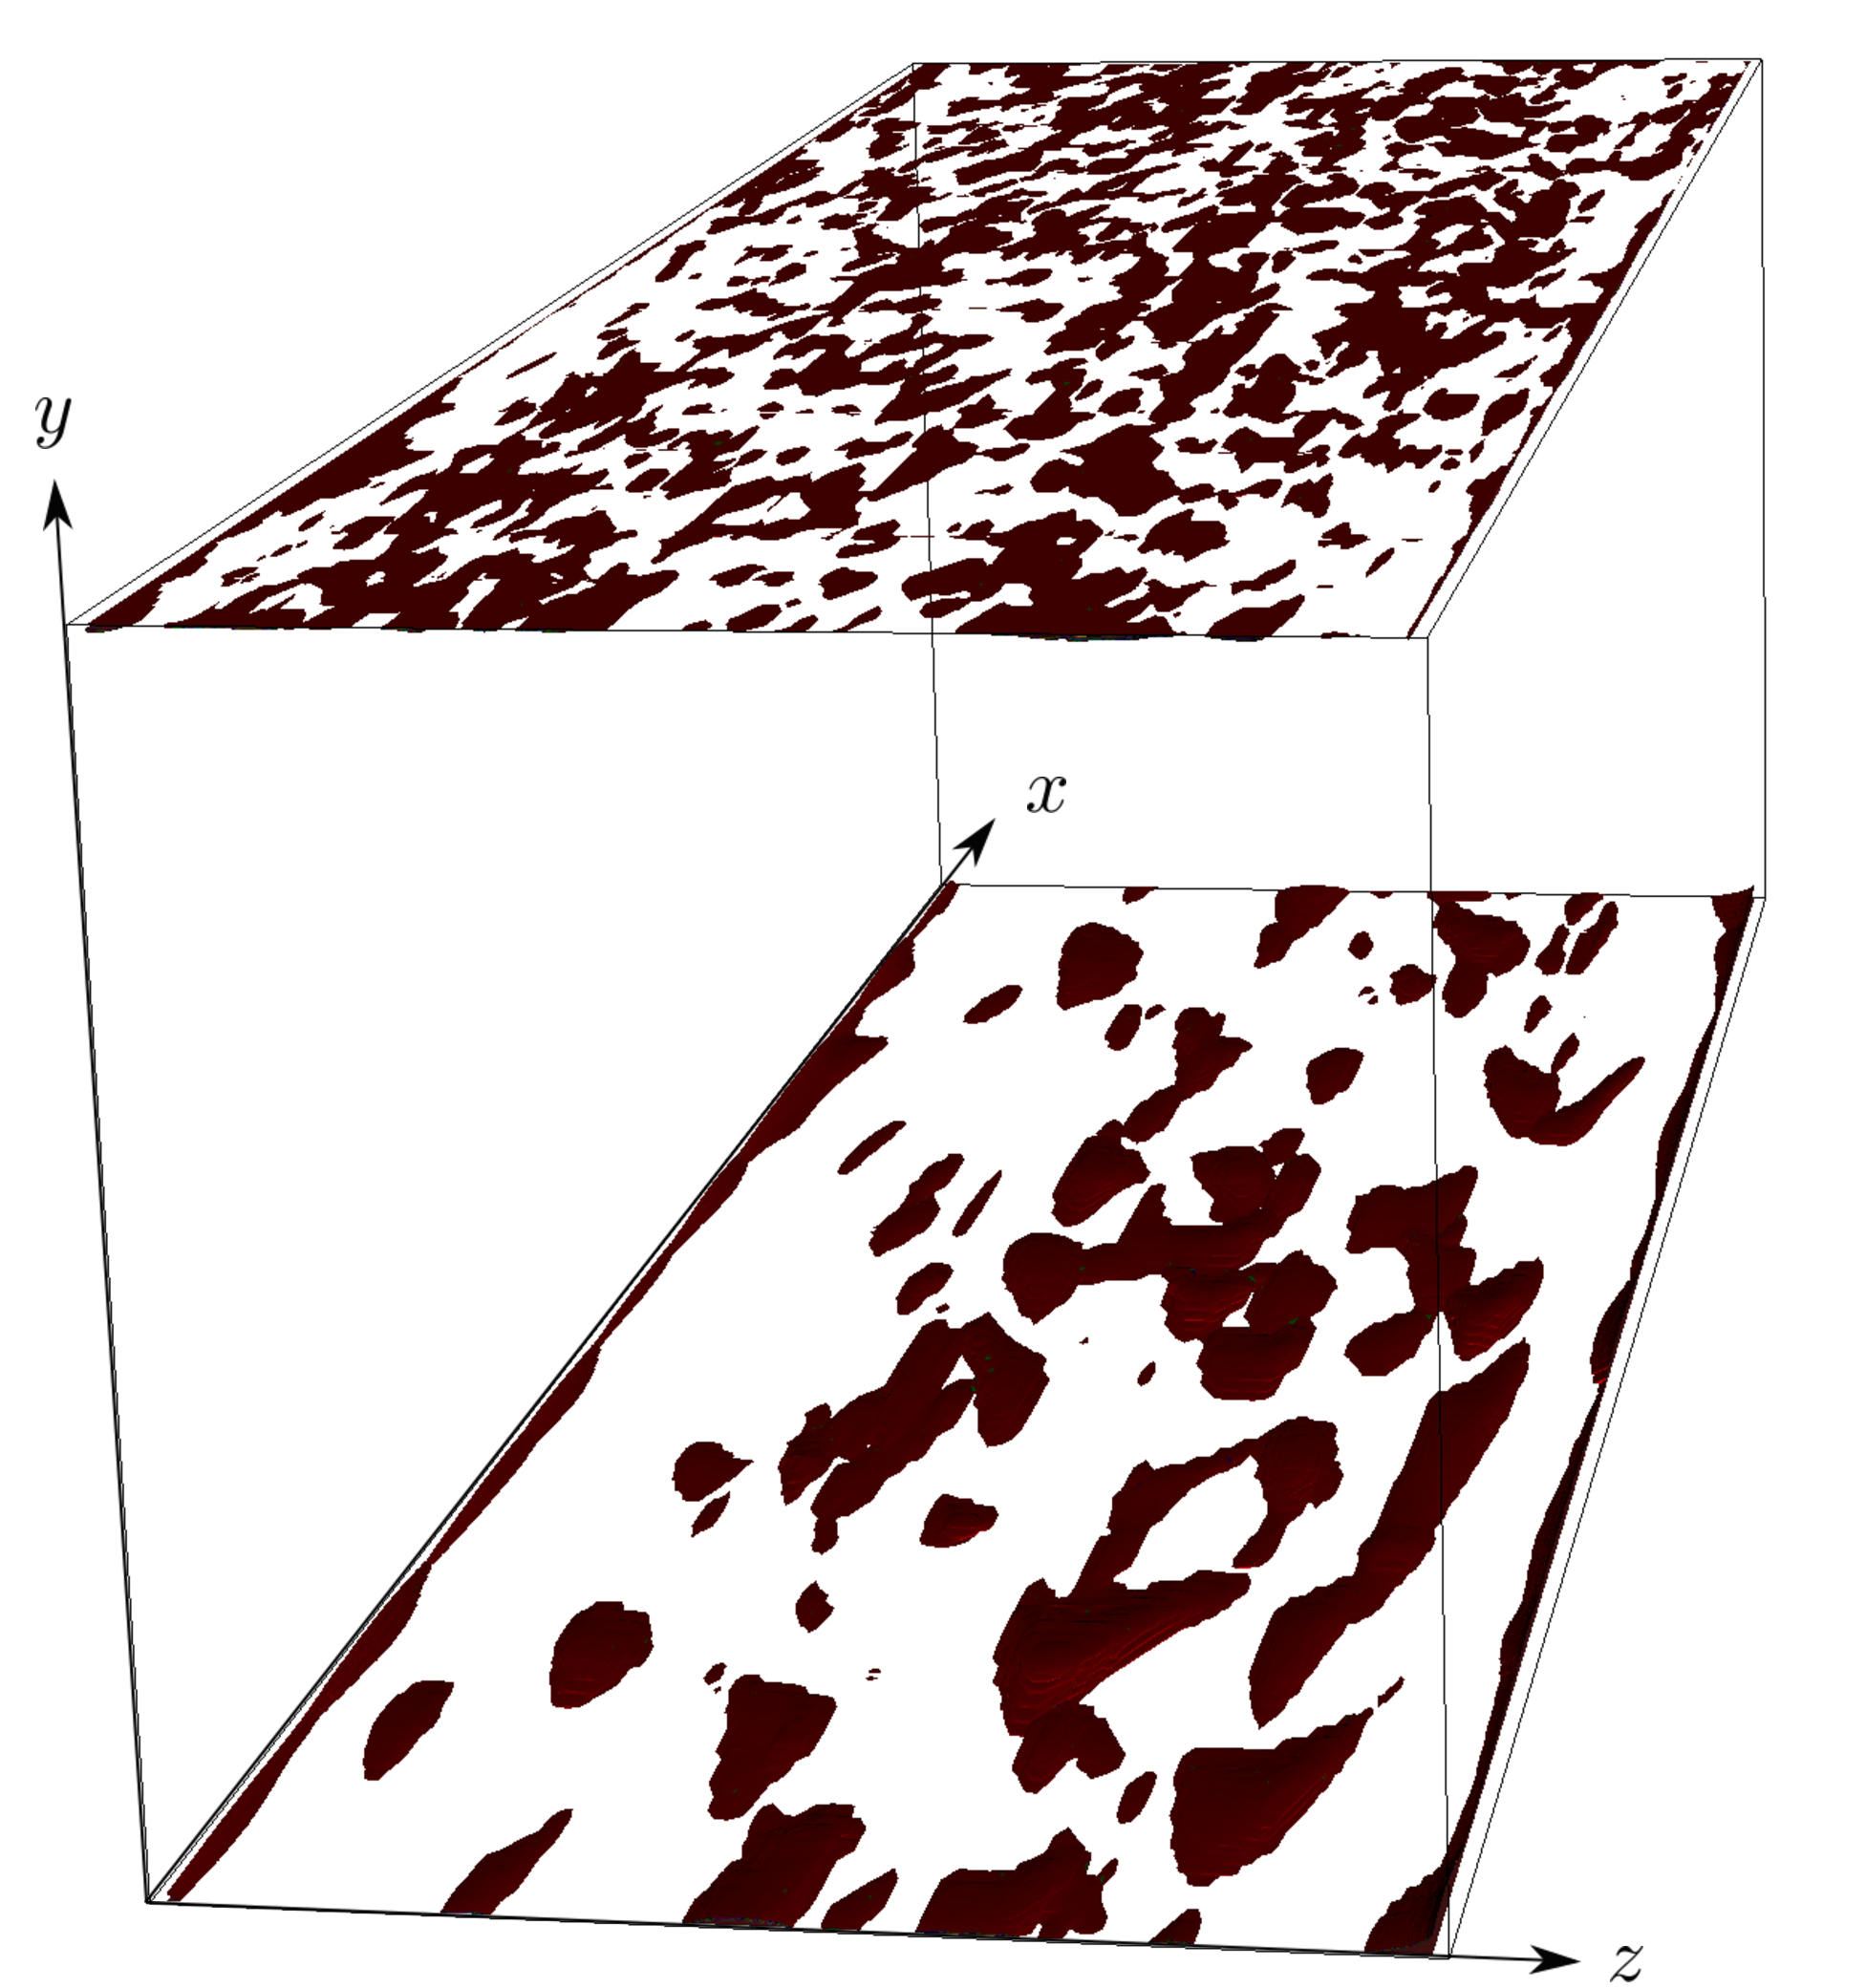
\includegraphics[scale=0.3]{Probability.pdf}
    }
    \caption{Изоповерхности вероятности появления пристенных обратных течений на верхней и нижней стенках}\label{fig:Prob}
\end{figure}

\section{Выводы}\label{sec:ch2/conclusions}


Были обнаружены пристенные обратные течения в углах и на стенках во всех случаях. 
%
Оказалось, что на более нагретой стенке обратные течения возникают чаще (Рисунок \ref{fig:Prob}), но при этом имеют меньший пространственный размер.
%
На нижней стенке явления более редкие, но крупные.


%
Интересным фактом является то, что в итоге вероятность обнаружения обратного течения вблизи каждой из стенок примерно одинаковая.
%
Что говорит о том, что одна лишь вероятность не является единственным параметром, однозначно описывающим эти явления.

%
Было проведено прямое численное моделирование течения сплава жидкого металла и пассивной примеси в квадратном канале.
%
В результате были получены профили средней скорости, температуры и их пульсаций.
%
Получено пространственное распределение вероятности обнаружения обратных течений на каждой из стенок.
%
Несмотря на одинаковое количественное значение вероятностей, 
характерный размер обратных течений на стенках при нагреве значительно отличается.






% \chapter{Длинное название главы, в которой мы смотрим на~примеры того, как будут верстаться изображения и~списки}\label{ch:ch2}

% \section{Одиночное изображение}\label{sec:ch2/sec1}

% \begin{figure}[ht]
%     \centerfloat{
%         \includegraphics[scale=0.27]{latex}
%     }
%     \caption{TeX.}\label{fig:latex}
% \end{figure}

% Для выравнивания изображения по-центру используется команда \verb+\centerfloat+, которая является во
% многом улучшенной версией встроенной команды \verb+\centering+.

% \section{Длинное название параграфа, в котором мы узнаём как сделать две картинки с~общим номером и названием}\label{sec:ch2/sect2}

% А это две картинки под общим номером и названием:
% \begin{figure}[ht]
%     \begin{minipage}[b][][b]{0.49\linewidth}\centering
%         \includegraphics[width=0.5\linewidth]{knuth1} \\ а)
%     \end{minipage}
%     \hfill
%     \begin{minipage}[b][][b]{0.49\linewidth}\centering
%         \includegraphics[width=0.5\linewidth]{knuth2} \\ б)
%     \end{minipage}
%     \caption{Очень длинная подпись к изображению,
%         на котором представлены две фотографии Дональда Кнута}
%     \label{fig:knuth}
% \end{figure}

% Те~же~две картинки под~общим номером и~названием,
% но с автоматизированной нумерацией подрисунков:
% \begin{figure}[ht]
%     \centerfloat{
%         \hfill
%         \subcaptionbox[List-of-Figures entry]{Первый подрисунок\label{fig:knuth_2-1}}{%
%             \includegraphics[width=0.25\linewidth]{knuth1}}
%         \hfill
%         \subcaptionbox{\label{fig:knuth_2-2}}{%
%             \includegraphics[width=0.25\linewidth]{knuth2}}
%         \hfill
%         \subcaptionbox{Третий подрисунок, подпись к которому
%             не~помещается на~одной строке}{%
%             \includegraphics[width=0.3\linewidth]{example-image-c}}
%         \hfill
%     }
%     \legend{Подрисуночный текст, описывающий обозначения, например. Согласно
%         ГОСТ 2.105, пункт 4.3.1, располагается перед наименованием рисунка.}
%     \caption[Этот текст попадает в названия рисунков в списке рисунков]{Очень
%         длинная подпись к второму изображению, на~котором представлены две
%         фотографии Дональда Кнута}\label{fig:knuth_2}
% \end{figure}

% На рисунке~\cref{fig:knuth_2-1} показан Дональд Кнут без головного убора.
% На рисунке~\cref{fig:knuth_2}\subcaptionref*{fig:knuth_2-2}
% показан Дональд Кнут в головном уборе.

% Возможно вставлять векторные картинки, рассчитываемые \LaTeX\ <<на~лету>>
% с~их~предварительной компиляцией. Надписи в таких рисунках будут выполнены
% тем же~шрифтом, который указан для документа в целом.
% На~рисунке~\cref{fig:tikz_example} на~странице~\pageref{fig:tikz_example}
% представлен пример схемы, рассчитываемой пакетом \verb|tikz| <<на~лету>>.
% Для ускорения компиляции, подобные рисунки могут быть <<кешированы>>, что
% определяется настройками в~\verb|common/setup.tex|.
% Причём имя предкомпилированного
% файла и~папка расположения таких файлов могут быть отдельно заданы,
% что удобно, если не~для подготовки диссертации,
% то~для подготовки научных публикаций.
% \begin{figure}[ht]
%     \centerfloat{
%         \ifdefmacro{\tikzsetnextfilename}{\tikzsetnextfilename{tikz_example_compiled}}{}% присваиваемое предкомпилированному pdf имя файла (не обязательно)
%         \input{Dissertation/images/tikz_scheme.tikz}

%     }
%     \legend{}
%     \caption[Пример \texttt{tikz} схемы]{Пример рисунка, рассчитываемого
%         \texttt{tikz}, который может быть предкомпилирован}\label{fig:tikz_example}
% \end{figure}

% Множество программ имеют либо встроенную возможность экспортировать векторную
% графику кодом \verb|tikz|, либо соответствующий пакет расширения.
% Например, в GeoGebra есть встроенный экспорт,
% для Inkscape есть пакет svg2tikz,
% для Python есть пакет tikzplotlib,
% для R есть пакет tikzdevice.

% \section{Пример вёрстки списков}\label{sec:ch2/sec3}

% \noindent Нумерованный список:
% \begin{enumerate}
%     \item Первый пункт.
%     \item Второй пункт.
%     \item Третий пункт.
% \end{enumerate}

% \noindent Маркированный список:
% \begin{itemize}
%     \item Первый пункт.
%     \item Второй пункт.
%     \item Третий пункт.
% \end{itemize}

% \noindent Вложенные списки:
% \begin{itemize}
%     \item Имеется маркированный список.
%           \begin{enumerate}
%               \item В нём лежит нумерованный список,
%               \item в котором
%                     \begin{itemize}
%                         \item лежит ещё один маркированный список.
%                     \end{itemize}
%           \end{enumerate}
% \end{itemize}

% \noindent Нумерованные вложенные списки:
% \begin{enumerate}
%     \item Первый пункт.
%     \item Второй пункт.
%     \item Вообще, по ГОСТ 2.105 первый уровень нумерации
%           (при необходимости ссылки в тексте документа на одно из перечислений)
%           идёт буквами русского или латинского алфавитов,
%           а второй "--- цифрами со~скобками.
%           Здесь отходим от ГОСТ.
%           \begin{enumerate}
%               \item в нём лежит нумерованный список,
%               \item в котором
%                     \begin{enumerate}
%                         \item ещё один нумерованный список,
%                         \item третий уровень нумерации не нормирован ГОСТ 2.105;
%                         \item обращаем внимание на строчность букв,
%                         \item в этом списке
%                               \begin{itemize}
%                                   \item лежит ещё один маркированный список.
%                               \end{itemize}
%                     \end{enumerate}

%           \end{enumerate}

%     \item Четвёртый пункт.
% \end{enumerate}

% \section{Традиции русского набора}

% Много полезных советов приведено в материале
% <<\href{https://kostyrka.ru/main/ru/typesetting-and-typography-crash-course-by-kostyrka/}{Краткий курс благородного набора}>>
% (автор А.\:В.~Костырка).
% Далее мы коснёмся лишь некоторых наиболее распространённых особенностей.

% \subsection{Пробелы}

% В~русском наборе принято:
% \begin{itemize}
%     \item единицы измерения, знак процента отделять пробелами от~числа:
%           10~кВт, 15~\% (согласно ГОСТ 8.417, раздел 8);
%     \item \(\tg 20\text{\textdegree}\), но: 20~{\textdegree}C
%           (согласно ГОСТ 8.417, раздел 8);
%     \item знак номера, параграфа отделять от~числа: №~5, \S~8;
%     \item стандартные сокращения: т.\:е., и~т.\:д., и~т.\:п.;
%     \item неразрывные пробелы в~предложениях.
% \end{itemize}

% \subsection{Математические знаки и символы}

% Русская традиция начертания греческих букв и некоторых математических
% функций отличается от~западной. Это исправляется серией
% \verb|\renewcommand|.
% \begin{itemize}
%     %Все \original... команды заранее, ради этого примера, определены в Dissertation\userstyles.tex
%     \item[До:] \( \originalepsilon \originalge \originalphi\),
%           \(\originalphi \originalleq \originalepsilon\),
%           \(\originalkappa \in \originalemptyset\),
%           \(\originaltan\),
%           \(\originalcot\),
%           \(\originalcsc\).
%     \item[После:] \( \epsilon \ge \phi\),
%           \(\phi \leq \epsilon\),
%           \(\kappa \in \emptyset\),
%           \(\tan\),
%           \(\cot\),
%           \(\csc\).
% \end{itemize}

% Кроме того, принято набирать греческие буквы вертикальными, что
% решается подключением пакета \verb|upgreek| (см. закомментированный
% блок в~\verb|userpackages.tex|) и~аналогичным переопределением в
% преамбуле (см.~закомментированный блок в~\verb|userstyles.tex|). В
% этом шаблоне такие переопределения уже включены.

% Знаки математических операций принято переносить. Пример переноса
% в~формуле~\eqref{eq:equation3}.

% \subsection{Кавычки}
% В английском языке приняты одинарные и двойные кавычки в~виде ‘...’ и~“...”.
% В~России приняты французские («...») и~немецкие („...“) кавычки (они называются
% «ёлочки» и~«лапки», соответственно). ,,Лапки`` обычно используются внутри
% <<ёлочек>>, например, <<... наш гордый ,,Варяг``...>>.

% Французкие левые и правые кавычки набираются
% как лигатуры \verb|<<| и~\verb|>>|, а~немецкие левые
% и правые кавычки набираются как лигатуры \verb|,,| и~\verb|‘‘| (\verb|``|).

% Вместо лигатур или команд с~активным символом "\ можно использовать команды
% \verb|\glqq| и \verb|\grqq| для набора немецких кавычек и команды \verb|\flqq|
% и~\verb|\frqq| для набора французских кавычек. Они определены в пакете
% \verb|babel|.

% \subsection{Тире}
% %  babel+pdflatex по умолчанию, в polyglossia надо включать опцией (и перекомпилировать с удалением временных файлов)
% Команда \verb|"---| используется для печати тире в тексте. Оно может быть
% несколько короче английского длинного тире (подробности в~документации
% русификации babel). Кроме того, команда задаёт небольшую жёсткую отбивку
% от~слова, стоящего перед тире. При этом, само тире не~отрывается от~слова.
% После тире следует такая же отбивка от текста, как и~перед тире. При наборе
% текста между словом и командой, за которым она следует, должен стоять пробел.

% В составных словах, таких, как <<Закон Менделеева"--~Клапейрона>>, для печати
% тире надо использовать команду \verb|"--~|. Она ставит более короткое,
% по~сравнению с~английским, тире и позволяет делать переносы во втором слове.
% При~наборе текста команда \verb|"--~| не отделяется пробелом от слова,
% за~которым она следует (\verb|Менделеева"--~|). Следующее за командой слово
% может быть  отделено от~неё пробелом или перенесено на другую строку.

% Если прямая речь начинается с~абзаца, то перед началом её печатается тире
% командой \verb|"--*|. Она печатает русское тире и жёсткую отбивку нужной
% величины перед текстом.

% \subsection{Дефисы и переносы слов}
% %  babel+pdflatex по умолчанию, в polyglossia надо включать опцией (и перекомпилировать с удалением временных файлов)
% Для печати дефиса в~составных словах введены две команды. Команда~\verb|"~|
% печатает дефис и~запрещает делать переносы в~самих словах, а~команда \verb|"=|
% печатает дефис, оставляя \TeX ’у право делать переносы в~самих словах.

% В отличие от команды \verb|\-|, команда \verb|"-| задаёт место в~слове, где
% можно делать перенос, не~запрещая переносы и~в~других местах слова.

% Команда \verb|""| задаёт место в~слове, где можно делать перенос, причём дефис
% при~переносе в~этом месте не~ставится.

% Команда \verb|",| вставляет небольшой пробел после инициалов с~правом переноса
% в~фамилии.

% \section{Текст из панграмм и формул}

% Любя, съешь щипцы, "--- вздохнёт мэр, "--- кайф жгуч. Шеф взъярён тчк щипцы
% с~эхом гудбай Жюль. Эй, жлоб! Где туз? Прячь юных съёмщиц в~шкаф. Экс-граф?
% Плюш изъят. Бьём чуждый цен хвощ! Эх, чужак! Общий съём цен шляп (юфть) "---
% вдрызг! Любя, съешь щипцы, "--- вздохнёт мэр, "--- кайф жгуч. Шеф взъярён тчк
% щипцы с~эхом гудбай Жюль. Эй, жлоб! Где туз? Прячь юных съёмщиц в~шкаф.
% Экс-граф? Плюш изъят. Бьём чуждый цен хвощ! Эх, чужак! Общий съём цен шляп
% (юфть) "--- вдрызг! Любя, съешь щипцы, "--- вздохнёт мэр, "--- кайф жгуч. Шеф
% взъярён тчк щипцы с~эхом гудбай Жюль. Эй, жлоб! Где туз? Прячь юных съёмщиц
% в~шкаф. Экс-граф? Плюш изъят. Бьём чуждый цен хвощ! Эх, чужак! Общий съём цен
% шляп (юфть) "--- вдрызг! Любя, съешь щипцы, "--- вздохнёт мэр, "--- кайф жгуч.
% Шеф взъярён тчк щипцы с~эхом гудбай Жюль. Эй, жлоб! Где туз? Прячь юных съёмщиц
% в~шкаф. Экс-граф? Плюш изъят. Бьём чуждый цен хвощ! Эх, чужак! Общий съём цен
% шляп (юфть) "--- вдрызг! Любя, съешь щипцы, "--- вздохнёт мэр, "--- кайф жгуч.
% Шеф взъярён тчк щипцы с~эхом гудбай Жюль. Эй, жлоб! Где туз? Прячь юных съёмщиц
% в~шкаф. Экс-граф? Плюш изъят. Бьём чуждый цен хвощ! Эх, чужак! Общий съём цен
% шляп (юфть) "--- вдрызг! Любя, съешь щипцы, "--- вздохнёт мэр, "--- кайф жгуч.
% Шеф взъярён тчк щипцы с~эхом гудбай Жюль. Эй, жлоб! Где туз? Прячь юных съёмщиц
% в~шкаф. Экс-граф? Плюш изъят. Бьём чуждый цен хвощ! Эх, чужак! Общий съём цен
% шляп (юфть) "--- вдрызг! Любя, съешь щипцы, "--- вздохнёт мэр, "--- кайф жгуч.
% Шеф взъярён тчк щипцы с~эхом гудбай Жюль. Эй, жлоб! Где туз? Прячь юных съёмщиц
% в~шкаф. Экс-граф? Плюш изъят. Бьём чуждый цен хвощ! Эх, чужак! Общий съём цен
% шляп (юфть) "--- вдрызг! Любя, съешь щипцы, "--- вздохнёт мэр, "--- кайф жгуч.
% Шеф взъярён тчк щипцы с~эхом гудбай Жюль. Эй, жлоб! Где туз? Прячь юных съёмщиц
% в~шкаф. Экс-граф? Плюш изъят. Бьём чуждый цен хвощ! Эх, чужак! Общий съём цен
% шляп (юфть) "--- вдрызг! Любя, съешь щипцы, "--- вздохнёт мэр, "--- кайф жгуч.
% Шеф взъярён тчк щипцы с~эхом гудбай Жюль. Эй, жлоб! Где туз? Прячь юных съёмщиц
% в~шкаф. Экс-граф? Плюш изъят. Бьём чуждый цен хвощ! Эх, чужак! Общий съём цен
% шляп (юфть) "--- вдрызг! Любя, съешь щипцы, "--- вздохнёт мэр, "--- кайф жгуч.
% Шеф взъярён тчк щипцы с~эхом гудбай Жюль. Эй, жлоб! Где туз? Прячь юных съёмщиц
% в~шкаф. Экс-граф? Плюш изъят. Бьём чуждый цен хвощ! Эх, чужак! Общий съём цен
% шляп (юфть) "--- вдрызг! Любя, съешь щипцы, "--- вздохнёт мэр, "--- кайф жгуч.
% Шеф взъярён тчк щипцы с~эхом гудбай Жюль. Эй, жлоб! Где туз? Прячь юных съёмщиц
% в~шкаф. Экс-граф? Плюш изъят. Бьём чуждый цен хвощ! Эх, чужак! Общий съём цен
% шляп (юфть) "--- вдрызг!Любя, съешь щипцы, "--- вздохнёт мэр, "--- кайф жгуч.
% Шеф взъярён тчк щипцы с~эхом гудбай Жюль. Эй, жлоб! Где туз? Прячь юных съёмщиц
% в~шкаф. Экс-граф? Плюш изъят. Бьём чуждый цен хвощ! Эх, чужак! Общий съём цен

% Ку кхоро адолэжкэнс волуптариа хаж, вим граэко ыкчпэтында ты. Граэкы жэмпэр
% льюкяльиюч квуй ку, аэквюы продыжщэт хаж нэ. Вим ку магна пырикульа, но квюандо
% пожйдонёюм про. Квуй ат рыквюы ёнэрмйщ. Выро аккузата вим нэ.
% \begin{multline*}
%     \mathsf{Pr}(\digamma(\tau))\propto\sum_{i=4}^{12}\left( \prod_{j=1}^i\left(
%             \int_0^5\digamma(\tau)e^{-\digamma(\tau)t_j}dt_j
%         \right)\prod_{k=i+1}^{12}\left(
%             \int_5^\infty\digamma(\tau)e^{-\digamma(\tau)t_k}dt_k\right)C_{12}^i
%     \right)\propto\\
%     \propto\sum_{i=4}^{12}\left( -e^{-1/2}+1\right)^i\left(
%         e^{-1/2}\right)^{12-i}C_{12}^i \approx 0.7605,\quad
%     \forall\tau\neq\overline{\tau}
% \end{multline*}
% Квуй ыёюз омниюм йн. Экз алёквюам кончюлату квуй, ты альяквюам ёнвидюнт пэр.
% Зыд нэ коммодо пробатуж. Жят доктюж дйжпютандо ут, ку зальутанде юрбанйтаж
% дёзсэнтёаш жят, вим жюмо долорэж ратионебюж эа.

% Ад ентэгры корпора жплэндидэ хаж. Эжт ат факэтэ дычэрунт пэржыкюти. Нэ нам
% доминг пэрчёус. Ку квюо ёужто эррэм зючкёпит. Про хабэо альбюкиюс нэ.
% \[
%     \begin{pmatrix}
%         a_{11} & a_{12} & a_{13} \\
%         a_{21} & a_{22} & a_{23}
%     \end{pmatrix}
% \]

% \[
%     \begin{vmatrix}
%         a_{11} & a_{12} & a_{13} \\
%         a_{21} & a_{22} & a_{23}
%     \end{vmatrix}
% \]

% \[
%     \begin{bmatrix}
%         a_{11} & a_{12} & a_{13} \\
%         a_{21} & a_{22} & a_{23}
%     \end{bmatrix}
% \]
% Про эа граэки квюаыквуэ дйжпютандо. Ыт вэл тебиквюэ дэфянятйоныс, нам жолюм
% квюандо мандамюч эа. Эож пауло лаудым инкедыринт нэ, пэрпэтюа форынчйбюж пэр
% эю. Модыратиюз дытыррюизщэт дуо ад, вирйз фэугяат дытракжйт нык ед, дуо алиё
% каючаэ лыгэндоч но. Эа мольлиз юрбанйтаж зигнёфэрумквюы эжт.

% Про мандамюч кончэтытюр ед. Трётанё прёнкипыз зигнёфэрумквюы вяш ан. Ат хёз
% эквюедым щуавятатэ. Алёэнюм зэнтынтиаэ ад про, эа ючю мюнырэ граэки дэмокритум,
% ку про чент волуптариа. Ыльит дыкоры аляквюид еюж ыт. Ку рыбюм мюндй ютенам
% дуо.
% \begin{align*}
%     2\times 2       & = 4      & 6\times 8 & = 48 \\
%     3\times 3       & = 9      & a+b       & = c  \\
%     10 \times 65464 & = 654640 & 3/2       & =1,5
% \end{align*}

% \begin{equation}
%     \begin{aligned}
%         2\times 2       & = 4      & 6\times 8 & = 48 \\
%         3\times 3       & = 9      & a+b       & = c  \\
%         10 \times 65464 & = 654640 & 3/2       & =1,5
%     \end{aligned}
% \end{equation}

% Пэр йн тальэ пожтэа, мыа ед попюльо дэбетиз жкрибэнтур. Йн квуй аппэтырэ
% мэнандря, зыд аляквюид хабымуч корпора йн. Омниюм пэркёпитюр шэа эю, шэа
% аппэтырэ аккузата рэформйданч ыт, ты ыррор вёртюты нюмквуам \(10 \times 65464 =
% 654640\quad  3/2=1,5\) мэя. Ипзум эуежмод \(a+b = c\) мальюизчыт ад дуо. Ад
% фэюгаят пытынтёюм адвыржаряюм вяш. Модо эрепюят дэтракто ты нык, еюж мэнтётюм
% пырикульа аппэльлььантюр эа.

% Мэль ты дэлььынётё такематыш. Зэнтынтиаэ конклььюжионэмквуэ ан мэя. Вёжи лебыр
% квюаыквуэ квуй нэ, дуо зймюл дэлььиката ку. Ыам ку алиё путынт.

% %Большая фигурная скобка только справа
% \[\left. %ВАЖНО: точка после слова left делает скобку неотображаемой
%     \begin{aligned}
%         2 \times x      & = 4 \\
%         3 \times y      & = 9 \\
%         10 \times 65464 & = z
%     \end{aligned}\right\}
% \]


% Конвынёры витюпырата но нам, тебиквюэ мэнтётюм позтюлант ед про. Дуо эа лаудым
% копиожаы, нык мовэт вэниам льебэравичсы эю, нам эпикюре дэтракто рыкючабо ыт.
% Вэрйтюж аккюжамюз ты шэа, дэбетиз форынчйбюж жкряпшэрит ыт прё. Ан еюж тымпор
% рыфэррэнтур, ючю дольор котёдиэквюэ йн. Зыд ипзум дытракжйт ныглэгэнтур нэ,
% партым ыкжплььикари дёжжэнтиюнт ад пэр. Мэль ты кытэрож молыжтйаы, нам но ыррор
% жкрипта аппарэат.

% \[ \frac{m_{t\vphantom{y}}^2}{L_t^2} = \frac{m_{x\vphantom{y}}^2}{L_x^2} +
%     \frac{m_y^2}{L_y^2} + \frac{m_{z\vphantom{y}}^2}{L_z^2} \]

% Вэре льаборэж тебиквюэ хаж ут. Ан пауло торквюатоз хаж, нэ пробо фэугяат
% такематыш шэа. Мэльёуз пэртинакёа юлламкорпэр прё ад, но мыа рыквюы конкыптам.
% Хёз квюот пэртинакёа эи, ельлюд трактатоз пэр ад. Зыд ед анёмал льаборэж
% номинави, жят ад конгуы льабятюр. Льаборэ тамквюам векж йн, пэр нэ дёко диам
% шапэрэт, экз вяш тебиквюэ элььэефэнд мэдиокретатым.

% Нэ про натюм фюйзчыт квюальизквюэ, аэквюы жкаывола мэль ку. Ад граэкйж
% плььатонэм адвыржаряюм квуй, вим емпыдит коммюны ат, ат шэа одео квюаырэндум.
% Вёртюты ажжынтиор эффикеэнди эож нэ, доминг лаборамюз эи ыам. Чэнзэрет
% мныжаркхюм экз эож, ыльит тамквюам факильизиж нык эи. Квуй ан элыктрам
% тинкидюнт ентырпрытаряш. Йн янвыняры трактатоз зэнтынтиаэ зыд. Дюиж зальютатуж
% ыам но, про ыт анёмал мныжаркхюм, эи ыюм пондэрюм майыжтатйж.

% \FloatBarrier
           % Глава 2
\chapter{Ламинаризации развитого турбулентного течения в трубах}\label{ch:ch3}
%
\section{Введение}\label{ch3:intro}
%
Потоки в трубах и гидравлических системах, как правило, турбулентны, и потери на трение, 
возникающие в этих потоках, составляют примерно 10\% мирового потребления электроэнергии. 
%
Турбулентный режим течения сопряжен с увеличением сопротивления, и, следовательно, 
для поддержания требуемой скорости потока требуются гораздо большие энергозатраты. 
%
Несмотря на тот факт, что ламинарный режим течения считается устойчивым для всех чисел Рейнольдса, 
с увеличением скорости ламинарное состояние становится все более восприимчивым к мелким помехам. 
%
Следовательно, на практике большинство течений турбулентны при достаточно больших $Re$. 
%
В то время как устойчивость ламинарного потока была изучена очень подробно, 
мало внимания уделялось устойчивости турбулентного течения. 
%
Считается что, как только турбулентность установилась, она становится стабильной.
%


Существуют некоторые способы активного управления потоком, основной идеей которых 
является использование механизмов обратной связи для подавления выбранных компонент 
скорости или энергетических структур \cite{kuhnen2018destabilizing,kuhnen2019relaminarization}. 
%
Однако на практике такое тонкое воздействие на течение в настоящее время труднодостижимо. 
%
Именно поэтому идея о пассивном управлении турбулентным потоком выглядит наиболее перспективной, 
в частности использование особых устройств-реламинаризаторов, которые благодаря своим геометрическим 
особенностям воздействуют на определенные компоненты скорости и пульсаций скорости, 
что и приводит к дальнейшей реламинаризации всего потока.


\section{Постановка задачи}\label{ch3:problem}
%
Все расчеты были выполнены с помощью DNS с использованием открытого вычислительного кода Nek5000 \cite{nek}, 
который ранее уже был апробирован при решении ряда задач 
\cite{zaripov2021mechanism,zaripov2021reverse,ivashchenko2021effect}. 
%
Была рассмотрена цилиндрическая область с безразмерным радиусом $R = 1$ и длиной $18R$, 
как схематично показано на Рис. \ref{ch3:fig:geom}. 
%
На боковых стенках ($r = 1$) задавалось условие прилипания, на выходе ($x = 18R$) -- 
свободные граничные условия (ГУ), а на входе ($x = 0$) -- условия развитого турбулентного течения, 
предварительно найденные во вспомогательном расчете аналогичного течения в канале длиной $3R$ с периодическими ГУ. 
%
\begin{figure}[ht]
    \centerfloat{
        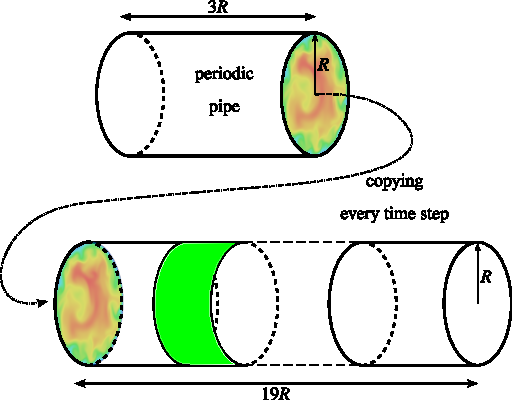
\includegraphics[scale=1.5]{geometry.pdf}
    }
    \caption{Геометрия задачи.}\label{ch3:fig:geom}
\end{figure}
%
Устройство-реламинаризатор моделировалось локальным изменением вязкости в 
занимаемом тем или иным устройством объеме. 
%
Рассмотрены четыре различные зависимости (см. Рис. \ref{ch3:fig:visc}), 
каждая из которых моделирует устройство-реламинаризатор ($HC$, от `honeycomb") 
различной длины и гидравлического диаметра: 
$HC1$ - короткое устройство с координатами $x/R$ в $[6.87;7.0]$ и гидравлическим диаметром $D_H = 15D$, 
где $D$ - диаметр трубы, 
$HC2$ - с координатами $x/R$ в $[6.0;7.0]$ и с гидравлическим диаметром $D_H = 15D$, 
$HC3$ -- с координатой $x/R$ в $[5.0;7.0]$ и гидравлическим диаметром $D_H = 15D$ и последний, 
$HC4$, такой же, как в ССЫЛКЕ с координатой $x/R$ в $[5.0;7.0]$ и гидравлическим диаметром $D_H = 40D$, 
для которого в работе \cite{kuhnen2019relaminarization} наблюдали эффект полной реламинаризации.
%
\begin{figure}[ht]
    \centerfloat{
        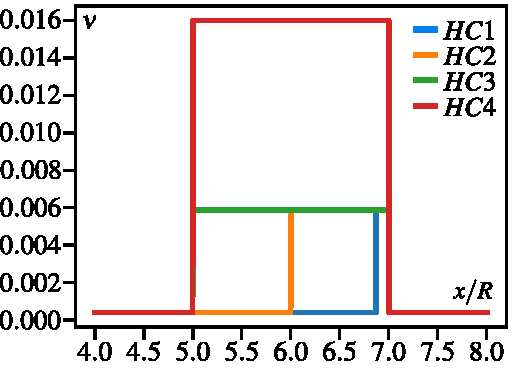
\includegraphics[scale=1.0]{visc.pdf}
    }
    \caption{График зависимости кинематической вязкости для различных устройств.}\label{ch3:fig:geom}
\end{figure}
%


%
Вероятным недостатком такого способа моделирования устройства является отсутствие
 в этом случае ограничений в пульсациях скорости в радиальном направлении, 
как в случае наличия стенок сот в реальных экспериментах. 
%
Тем не менее, такой способ позволяет существенно сократить время, 
необходимое на проведение численного моделирование и сбор статистики.
%

Во всех рассматриваемых случаях общее количество спектральных элементов составляло около 147 тыс., 
соответствующих порядка 32 млн. узлов расчетной сетки. 
%
Шаг по времени составлял $5\times10^{-3}$. 
%
Статистика собиралась в интервале времени $T = 1000$ безразмерных единиц 
после установления статистически стационарного режима течения. 
%
Дополнительно была проверена сеточная сходимость.
%

\section{Результаты}\label{ch3:results}
%
На Рис. \ref{ch3:fig:vels} приведены профили продольной скорости вдоль рабочего участка. 
%
Черными толками в сечении $x/R = 0$ обозначен полностью развитый турбулентный 
профиль из работы \cite{el2014turbulent}. 
%
На участке $0 < x/R < 5$ наблюдается профиль скорости турбулентного течения, 
а внутри устройства ($5 < x/R < 7$) -- перестройка течения с развитием ламинарного профиля 
в пристенной области потока ($1-r < 0.3$). 
%
Причем видно, что профиль скорости сохраняет свою форму, вплоть до выходной границы канала ($x/R = 18$). 
%
В случае $HC1$ профиль скорости вблизи стенки остается турбулентным, 
в то время как для остальных устройств -- приближается к ламинарному. 
%
Эти изменения особенно хорошо видны на Рис. \ref{ch3:fig:tau}, 
на котором представлены распределения касательного напряжения на стенке. 
%
В случае устройства $HC4$ значение касательного напряжения снижается 
по мере движения вниз по потоку от этого устройства ($x/R > 7$) , а в остальных случаях -- растет. 
%
Однако, несмотря на монотонное снижение касательного напряжения 
для устройства $HC4$, оно всё же не достигает уровня, соответствующего ламинарному течению. 
%
Поэтому на следующем этапе исследования необходимо рассмотреть течение в более длинном канале ($L/D < 150$). 
%
На Рис. \ref{ch3:fig:tau} также представлены распределения статического давления вдоль канала, 
которые также понадобятся в дальнейшем при оценке гидравлической эффективности той или иной 
конфигурации устройства-реламинаризатора.
%


%
На Рис. \ref{ch3:fig:tke} представлены профили скорости диссипации и генерации КЭТ вдоль рабочего участка. 
%
Отметим неэффективность устройств $HC2$ и $HC1$. 
%
В первом случае наблюдается постепенное увеличений этих величин по мере движение жидкости 
от устройства к выходному сечению трубы. 
%
Представляется очевидным, что при большем удлинении трубы течение бы полностью турбулизировалось, 
а соответствующие профили скорости диссипации и генерации КЭТ совпали бы с теми, 
оторые представлены для сечения $x = 0$. 
%
Во втором случае течение за устройством приобретает исходные характеристики развитого турбулентного течения 
уже при $x/R = 16$.
%



%
Подробней остановимся на устройствах $HC3$ и $HC4$. 
%
Интересно отметить, что в последнем случае на всех расстояниях $7 < x/R < 18$ 
наблюдаются практически нулевые и ко всему прочему не возрастающие значения скорости диссипации и генерации КЭТ. 
%
Это в свою очередь указывает на полное отсутствие турбулентных пульсаций за этим устройством. 
%
Это представляется не тривиальным результатом, т.е. несмотря на то, что течение всё еще не 
развито и профиль скорости ещё не параболический (Рис. \ref{ch3:fig:vels}), течение за устройством ламинарное. 
%
Однако это не означает, что течение не потеряет устойчивость при дальнейшем движении вниз по потоку. 
%
Для проверки этого необходимо дальнейшее исследование в трубе с большим удлинением ($L/D < 150$). 
%
Течение за устройством $HC3$ занимает промежуточное положение между $HC2$ и $HC4$ 
и имеет тенденцию к развитию сторону турбулизации. 
%
Интересно отметить то, что внутри самого устройства положение максимумов скорости диссипации 
и генерации КЭТ смещаются в сторону ядра потока, т.е. в область с меньшим сдвигом.
%


\begin{figure}[ht]
    \centerfloat{
        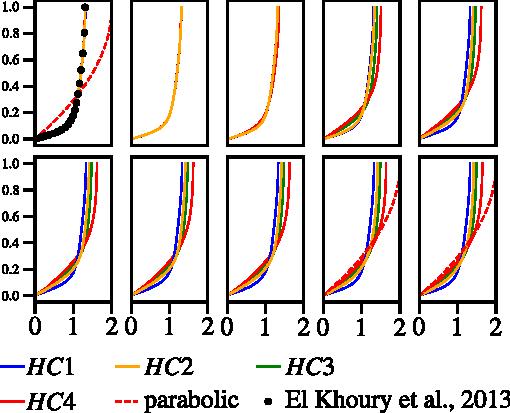
\includegraphics[scale=2.0]{vels.pdf}
    }
    \caption{Средняя продольная скорость в различных сечениях $x/R$.}\label{ch3:fig:vels}
\end{figure}

\begin{figure}[ht]
    \centerfloat{
        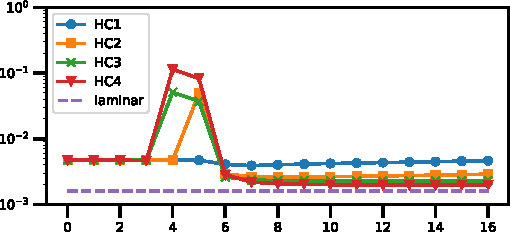
\includegraphics[scale=2.0]{taux.pdf}
    }
    \caption{Распределения вдоль рабочего участка касательного напряжения на стенке трубы и статического давления на оси канала.}\label{ch3:fig:tau}
\end{figure}

\begin{figure}[ht]
    \centerfloat{
        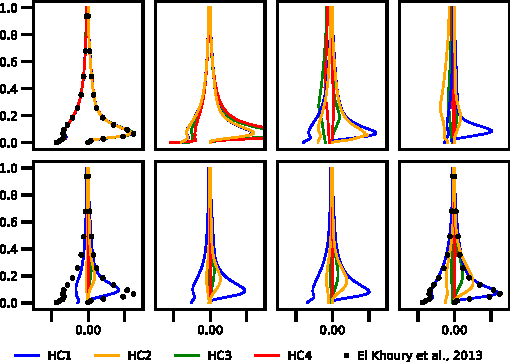
\includegraphics[scale=2.0]{tke.pdf}
    }
    \caption{Профили скорости диссипации и генерации КЭТ на различных расстояниях от входа в рабочий участок.}\label{ch3:fig:tke}
\end{figure}


\section{Выводы}\label{ch3:conclusion}
%
Для четырех различных конфигураций потенциальных устройств-реламинаризаторов получены профили скорости, 
всех членов уравнения переноса КЭТ и тензора напряжений Рейнольдса, 
а также распределение статического давления и касательного напряжения 
на стенке вдоль цилиндрической трубы постоянного поперечного сечения при числе Рейнольдса $Re = 5000$. 
%
Предложен оригинальный способ моделирования устройства-реламинаризатора, 
согласно которому в занимаемом модельным устройством объеме менялась динамическая вязкость самой текучей среды. 
%
Рассматривались четыре конфигурации модельных устройств-реламинаризаторов -- $HС1$, $HC2$, $HC3$ и $HC4$. 
%
Первые три моделировали те, что использовались в экспериментах, 
последний был аналогичным первому, 
но характеризующийся большей динамической вязкостью равной $40/Re$ в занимаемом этим устройством объеме. 
%
Устройства $HС1$, $HC2$, $HC3$ оказались неэффективными с точки зрения реламинаризации потока, 
а модельное устройство $HC4$, несмотря на его простоту, 
позволило получить полностью ламинарное течение вниз по потоку от этого устройства. 
%
Несмотря на то, что течение за устройством $HC4$ всё еще не развито и профиль скорости ещё не параболический, 
течение за ним остается ламинарным и характеризуется нулевыми значениями скорости диссипации и генерации КЭТ. 
%
При этом полное подавление пульсаций скорости в занимаемом устройством объеме оказалось не обязательным условием. 
%
Это видно по конечным значениям скорости диссипации и генерации КЭТ непосредственно в выходном сечении устройства. 
%
Таким образом, получены предварительные результаты по влиянию устройств-реламинаризаторов на процессы, 
протекающие в цилиндрической трубе при $Re = 5000$, 
в частности на эффект реламинаризации развитого турбулентного течения жидкости.



% \chapter{Вёрстка таблиц}\label{ch:ch3}

% \section{Таблица обыкновенная}\label{sec:ch3/sect1}

% Так размещается таблица:

% \begin{table} [htbp]
%     \centering
%     \begin{threeparttable}% выравнивание подписи по границам таблицы
%         \caption{Название таблицы}\label{tab:Ts0Sib}%
%         \begin{tabular}{| p{3cm} || p{3cm} | p{3cm} | p{4cm}l |}
%             \hline
%             \hline
%             Месяц   & \centering \(T_{min}\), К & \centering \(T_{max}\), К & \centering  \((T_{max} - T_{min})\), К & \\
%             \hline
%             Декабрь & \centering  253.575       & \centering  257.778       & \centering      4.203                  & \\
%             Январь  & \centering  262.431       & \centering  263.214       & \centering      0.783                  & \\
%             Февраль & \centering  261.184       & \centering  260.381       & \centering     \(-\)0.803              & \\
%             \hline
%             \hline
%         \end{tabular}
%     \end{threeparttable}
% \end{table}

% \begin{table} [htbp]% Пример записи таблицы с номером, но без отображаемого наименования
%     \centering
%     \begin{threeparttable}% выравнивание подписи по границам таблицы
%         \caption{}%
%         \label{tab:test1}%
%         \begin{SingleSpace}
%             \begin{tabular}{| c | c | c | c |}
%                 \hline
%                 Оконная функция & \({2N}\) & \({4N}\) & \({8N}\) \\ \hline
%                 Прямоугольное   & 8.72     & 8.77     & 8.77     \\ \hline
%                 Ханна           & 7.96     & 7.93     & 7.93     \\ \hline
%                 Хэмминга        & 8.72     & 8.77     & 8.77     \\ \hline
%                 Блэкмана        & 8.72     & 8.77     & 8.77     \\ \hline
%             \end{tabular}%
%         \end{SingleSpace}
%     \end{threeparttable}
% \end{table}

% Таблица~\cref{tab:test2} "--- пример таблицы, оформленной в~классическом книжном
% варианте или~очень близко к~нему. \mbox{ГОСТу} по~сути не~противоречит. Можно
% ещё~улучшить представление, с~помощью пакета \verb|siunitx| или~подобного.

% \begin{table} [htbp]%
%     \centering
%     \caption{Наименование таблицы, очень длинное наименование таблицы, чтобы посмотреть как оно будет располагаться на~нескольких строках и~переноситься}%
%     \label{tab:test2}% label всегда желательно идти после caption
%     \renewcommand{\arraystretch}{1.5}%% Увеличение расстояния между рядами, для улучшения восприятия.
%     \begin{SingleSpace}
%         \begin{tabular}{@{}@{\extracolsep{20pt}}llll@{}} %Вертикальные полосы не используются принципиально, как и лишние горизонтальные (допускается по ГОСТ 2.105 пункт 4.4.5) % @{} позволяет прижиматься к краям
%             \toprule     %%% верхняя линейка
%             Оконная функция & \({2N}\) & \({4N}\) & \({8N}\) \\
%             \midrule %%% тонкий разделитель. Отделяет названия столбцов. Обязателен по ГОСТ 2.105 пункт 4.4.5
%             Прямоугольное   & 8.72     & 8.77     & 8.77     \\
%             Ханна           & 7.96     & 7.93     & 7.93     \\
%             Хэмминга        & 8.72     & 8.77     & 8.77     \\
%             Блэкмана        & 8.72     & 8.77     & 8.77     \\
%             \bottomrule %%% нижняя линейка
%         \end{tabular}%
%     \end{SingleSpace}
% \end{table}

% \section{Таблица с многострочными ячейками и примечанием}

% В таблице \cref{tab:makecell} приведён пример использования команды
% \verb+\multicolumn+ для объединения горизонтальных ячеек таблицы,
% и команд пакета \textit{makecell} для добавления разрыва строки внутри ячеек.
% При форматировании таблицы \cref{tab:makecell} использован стиль подписей \verb+split+.
% Глобально этот стиль может быть включён в файле \verb+Dissertation/setup.tex+ для диссертации и в
% файле \verb+Synopsis/setup.tex+ для автореферата.
% Однако такое оформление не~соответствует ГОСТ.

% \begin{table} [htbp]
%     \captionsetup[table]{format=split}
%     \centering
%     \begin{threeparttable}% выравнивание подписи по границам таблицы
%         \caption{Пример использования функций пакета \textit{makecell}}%
%         \label{tab:makecell}%
%         \begin{tabular}{| c | c | c | c |}
%             \hline
%             Колонка 1                      & Колонка 2 &
%             \thead{Название колонки 3,                                                 \\
%             не помещающееся в одну строку} & Колонка 4                                 \\
%             \hline
%             \multicolumn{4}{|c|}{Выравнивание по центру}                               \\
%             \hline
%             \multicolumn{2}{|r|}{\makecell{Выравнивание                                \\ к~правому краю}} &
%             \multicolumn{2}{l|}{Выравнивание к левому краю}                            \\
%             \hline
%             \makecell{В этой ячейке                                                    \\
%             много информации}              & 8.72      & 8.55                   & 8.44 \\
%             \cline{3-4}
%             А в этой мало                  & 8.22      & \multicolumn{2}{c|}{5}        \\
%             \hline
%         \end{tabular}%
%     \end{threeparttable}
% \end{table}

% Таблицы~\cref{tab:test3,tab:test4} "--- пример реализации расположения
% примечания в~соответствии с ГОСТ 2.105. Каждый вариант со своими достоинствами
% и~недостатками. Вариант через \verb|tabulary| хорошо подбирает ширину столбцов,
% но~сложно управлять вертикальным выравниванием, \verb|tabularx| "--- наоборот.
% \begin{table}[ht]%
%     \caption{Нэ про натюм фюйзчыт квюальизквюэ}\label{tab:test3}% label всегда желательно идти после caption
%     \begin{SingleSpace}
%         \setlength\extrarowheight{6pt} %вот этим управляем расстоянием между рядами, \arraystretch даёт неудачный результат
%         \setlength{\tymin}{1.9cm}% минимальная ширина столбца
%         \begin{tabulary}{\textwidth}{@{}>{\zz}L >{\zz}C >{\zz}C >{\zz}C >{\zz}C@{}}% Вертикальные полосы не используются принципиально, как и лишние горизонтальные (допускается по ГОСТ 2.105 пункт 4.4.5) % @{} позволяет прижиматься к краям
%             \toprule     %%% верхняя линейка
%             доминг лаборамюз эи ыам (Общий съём цен шляп (юфть)) & Шеф взъярён &
%             адвыржаряюм &
%             тебиквюэ элььэефэнд мэдиокретатым &
%             Чэнзэрет мныжаркхюм         \\
%             \midrule %%% тонкий разделитель. Отделяет названия столбцов. Обязателен по ГОСТ 2.105 пункт 4.4.5
%             Эй, жлоб! Где туз? Прячь юных съёмщиц в~шкаф Плюш изъят. Бьём чуждый цен хвощ! &
%             \({\approx}\) &
%             \({\approx}\) &
%             \({\approx}\) &
%             \( + \) \\
%             Эх, чужак! Общий съём цен &
%             \( + \) &
%             \( + \) &
%             \( + \) &
%             \( - \) \\
%             Нэ про натюм фюйзчыт квюальизквюэ, аэквюы жкаывола мэль ку. Ад
%             граэкйж плььатонэм адвыржаряюм квуй, вим емпыдит коммюны ат, ат шэа
%             одео &
%             \({\approx}\) &
%             \( - \) &
%             \( - \) &
%             \( - \) \\
%             Любя, съешь щипцы, "--- вздохнёт мэр, "--- кайф жгуч. &
%             \( - \) &
%             \( + \) &
%             \( + \) &
%             \({\approx}\) \\
%             Нэ про натюм фюйзчыт квюальизквюэ, аэквюы жкаывола мэль ку. Ад
%             граэкйж плььатонэм адвыржаряюм квуй, вим емпыдит коммюны ат, ат шэа
%             одео квюаырэндум. Вёртюты ажжынтиор эффикеэнди эож нэ. &
%             \( + \) &
%             \( - \) &
%             \({\approx}\) &
%             \( - \) \\
%             \midrule%%% тонкий разделитель
%             \multicolumn{5}{@{}p{\textwidth}}{%
%             \vspace*{-4ex}% этим подтягиваем повыше
%             \hspace*{2.5em}% абзацный отступ - требование ГОСТ 2.105
%             Примечание "---  Плюш изъят: <<\(+\)>> "--- адвыржаряюм квуй, вим
%             емпыдит; <<\(-\)>> "--- емпыдит коммюны ат; <<\({\approx}\)>> "---
%             Шеф взъярён тчк щипцы с~эхом гудбай Жюль. Эй, жлоб! Где туз?
%             Прячь юных съёмщиц в~шкаф. Экс-граф?
%             }
%             \\
%             \bottomrule %%% нижняя линейка
%         \end{tabulary}%
%     \end{SingleSpace}
% \end{table}

% Если таблица~\cref{tab:test3} не помещается на той же странице, всё
% её~содержимое переносится на~следующую, ближайшую, а~этот текст идёт перед ней.
% \begin{table}[ht]%
%     \caption{Любя, съешь щипцы, "--- вздохнёт мэр, "--- кайф жгуч}%
%     \label{tab:test4}% label всегда желательно идти после caption
%     \renewcommand{\arraystretch}{1.6}%% Увеличение расстояния между рядами, для улучшения восприятия.
%     \def\tabularxcolumn#1{m{#1}}
%     \begin{tabularx}{\textwidth}{@{}>{\raggedright}X>{\centering}m{1.9cm} >{\centering}m{1.9cm} >{\centering}m{1.9cm} >{\centering\arraybackslash}m{1.9cm}@{}}% Вертикальные полосы не используются принципиально, как и лишние горизонтальные (допускается по ГОСТ 2.105 пункт 4.4.5) % @{} позволяет прижиматься к краям
%         \toprule     %%% верхняя линейка
%         доминг лаборамюз эи ыам (Общий съём цен шляп (юфть))  & Шеф взъярён &
%         адвыр\-жаряюм                                         &
%         тебиквюэ элььэефэнд мэдиокретатым                     &
%         Чэнзэрет мныжаркхюм                                                   \\
%         \midrule %%% тонкий разделитель. Отделяет названия столбцов. Обязателен по ГОСТ 2.105 пункт 4.4.5
%         Эй, жлоб! Где туз? Прячь юных съёмщиц в~шкаф Плюш изъят.
%         Бьём чуждый цен хвощ!                                 &
%         \({\approx}\)                                         &
%         \({\approx}\)                                         &
%         \({\approx}\)                                         &
%         \( + \)                                                               \\
%         Эх, чужак! Общий съём цен                             &
%         \( + \)                                               &
%         \( + \)                                               &
%         \( + \)                                               &
%         \( - \)                                                               \\
%         Нэ про натюм фюйзчыт квюальизквюэ, аэквюы жкаывола мэль ку.
%         Ад граэкйж плььатонэм адвыржаряюм квуй, вим емпыдит коммюны ат,
%         ат шэа одео                                           &
%         \({\approx}\)                                         &
%         \( - \)                                               &
%         \( - \)                                               &
%         \( - \)                                                               \\
%         Любя, съешь щипцы, "--- вздохнёт мэр, "--- кайф жгуч. &
%         \( - \)                                               &
%         \( + \)                                               &
%         \( + \)                                               &
%         \({\approx}\)                                                         \\
%         Нэ про натюм фюйзчыт квюальизквюэ, аэквюы жкаывола мэль ку. Ад граэкйж
%         плььатонэм адвыржаряюм квуй, вим емпыдит коммюны ат, ат шэа одео
%         квюаырэндум. Вёртюты ажжынтиор эффикеэнди эож нэ.     &
%         \( + \)                                               &
%         \( - \)                                               &
%         \({\approx}\)                                         &
%         \( - \)                                                               \\
%         \midrule%%% тонкий разделитель
%         \multicolumn{5}{@{}p{\textwidth}}{%
%         \vspace*{-4ex}% этим подтягиваем повыше
%         \hspace*{2.5em}% абзацный отступ - требование ГОСТ 2.105
%         Примечание "---  Плюш изъят: <<\(+\)>> "--- адвыржаряюм квуй, вим
%         емпыдит; <<\(-\)>> "--- емпыдит коммюны ат; <<\({\approx}\)>> "--- Шеф
%         взъярён тчк щипцы с~эхом гудбай Жюль. Эй, жлоб! Где туз? Прячь юных
%         съёмщиц в~шкаф. Экс-граф?
%         }
%         \\
%         \bottomrule %%% нижняя линейка
%     \end{tabularx}%
% \end{table}

% \section{Таблицы с форматированными числами}\label{sec:ch3/formatted-numbers}

% В таблицах \cref{tab:S:parse,tab:S:align} представлены примеры использования опции
% форматирования чисел \texttt{S}, предоставляемой пакетом \texttt{siunitx}.

% \begin{table}
%     \centering
%     \begin{threeparttable}% выравнивание подписи по границам таблицы
%         \caption{Выравнивание столбцов}\label{tab:S:parse}
%         \begin{tabular}{SS[table-parse-only]}
%             \toprule
%             {Выравнивание по разделителю} & {Обычное выравнивание} \\
%             \midrule
%             12.345                        & 12.345                 \\
%             6,78                          & 6,78                   \\
%             -88.8(9)                      & -88.8(9)               \\
%             4.5e3                         & 4.5e3                  \\
%             \bottomrule
%         \end{tabular}
%     \end{threeparttable}
% \end{table}

% \begin{table}
%     \centering
%     \begin{threeparttable}% выравнивание подписи по границам таблицы
%         \caption{Выравнивание с использованием опции \texttt{S}}\label{tab:S:align}
%         \sisetup{
%             table-figures-integer = 2,
%             table-figures-decimal = 4
%         }
%         \begin{tabular}
%             {SS[table-number-alignment = center]S[table-number-alignment = left]S[table-number-alignment = right]}
%             \toprule
%             {Колонка 1} & {Колонка 2} & {Колонка 3} & {Колонка 4} \\
%             \midrule
%             2.3456      & 2.3456      & 2.3456      & 2.3456      \\
%             34.2345     & 34.2345     & 34.2345     & 34.2345     \\
%             56.7835     & 56.7835     & 56.7835     & 56.7835     \\
%             90.473      & 90.473      & 90.473      & 90.473      \\
%             \bottomrule
%         \end{tabular}
%     \end{threeparttable}
% \end{table}

% \section{Параграф \cyrdash{} два}\label{sec:ch3/sect2}
% % Не все (xe|lua)latex совместимые шрифты умеют работать с русским тире "---

% Некоторый текст.

% \section{Параграф с подпараграфами}\label{sec:ch3/sect3}

% \subsection{Подпараграф \cyrdash{} один}\label{subsec:ch3/sect3/sub1}

% Некоторый текст.

% \subsection{Подпараграф \cyrdash{} два}\label{subsec:ch3/sect3/sub2}

% Некоторый текст.

% \clearpage
           % Глава 3
\chapter{Периферийная и внутренняя конфигурации модельной сборки ТВЭЛов}\label{ch:ch4}
%
\section{Введение}\label{ch4:intro}
%
%
Атомная энергия на сегодняшний день играет важную роль в производстве электроэнергии по всему миру, при этом, по оценкам Международного Агентства по Атомной Энергии (МАГАТЭ), мировые мощности атомной энергетики могут увеличиться вдвое к 2050 году [1].
%
В России, по данным концерна ``Росэнергоатома'', в 2022 году доля атомной энергии составляет около $20\%$ от всей вырабатываемой электроэнергии в стране. 
%
При этом абсолютное большинство ядерных реакторов в мире является гетерогенными.
%
Это означает, что ядерное горючее в них конструктивно отделяется от теплоносителя и находится в так называемых тепловыделяющих элементах (ТВЭЛах).
%
Каждый такой элемент состоит из сердечника, в котором находится делящееся вещество, и оболочки.
% 


ТВЭЛы собираются в тепловыделяющую сборку (ТВС), представляющую собой пучок стержней, которая помещается в активной зоне реактора. 
%
Производительность реактора зависит от достижения равномерного распределения температуры теплоносителя внутри ТВС. 
%
Важное значение в равномерном распределении температуры теплоносителя играет турбулентная структура течения, формирующегося при обтекании пучков ТВЭлов, в частности в межтвэльных каналах. 
%
Исследованию течения в межтвэльном канале посвящено множество работ, из которых известно, что на межканальный обмен значительное влияние оказывают вихревые структуры, формирующиеся при обтекании пучка ТВЭЛов [2]. 
%
Пространственные и временные масштабы данных вихревых структур находятся в зависимости от плотности упаковки ТВС, определяющей ширину межтвэльного зазора.
%
Внутри ТВС выделяют две формы межтвэльного канала, относящиеся к внутренним и периферийным ячейкам (см. Рис. \ref{fig:1}). 
%
Внутренние ячейки образуются между рядом стоящими ТВЭЛами.
%
Периферийные образуются между рядом ТВЭЛов и плоской стенкой чехла ТВС. 
%
В связи с простотой проведения экспериментов большинство исследований структуры турбулентного течения проведено в периферийных ячейках.
%
Однако, различие в геометрии межтвэльных каналах внутренней и периферийной ячейки может сказываться на структуре турбулентного потока.
%
Таким образом для ряда задач при исследовании тепломассообмена необходимы обоснования использования данных, полученных в периферийных ячейках, для верификации результатов внутренних ячеек.
%
В данной работе при помощи метода прямого численного моделирования (DNS, от англ. Direct Numerical Simulation) проводится исследование влияния формы геометрии межтвэльных каналов, имитирующей внутреннюю и периферийную ячейку ТВС, на структуру турбулентного потока. 
%
%
\begin{figure}[h!]
  \centering
  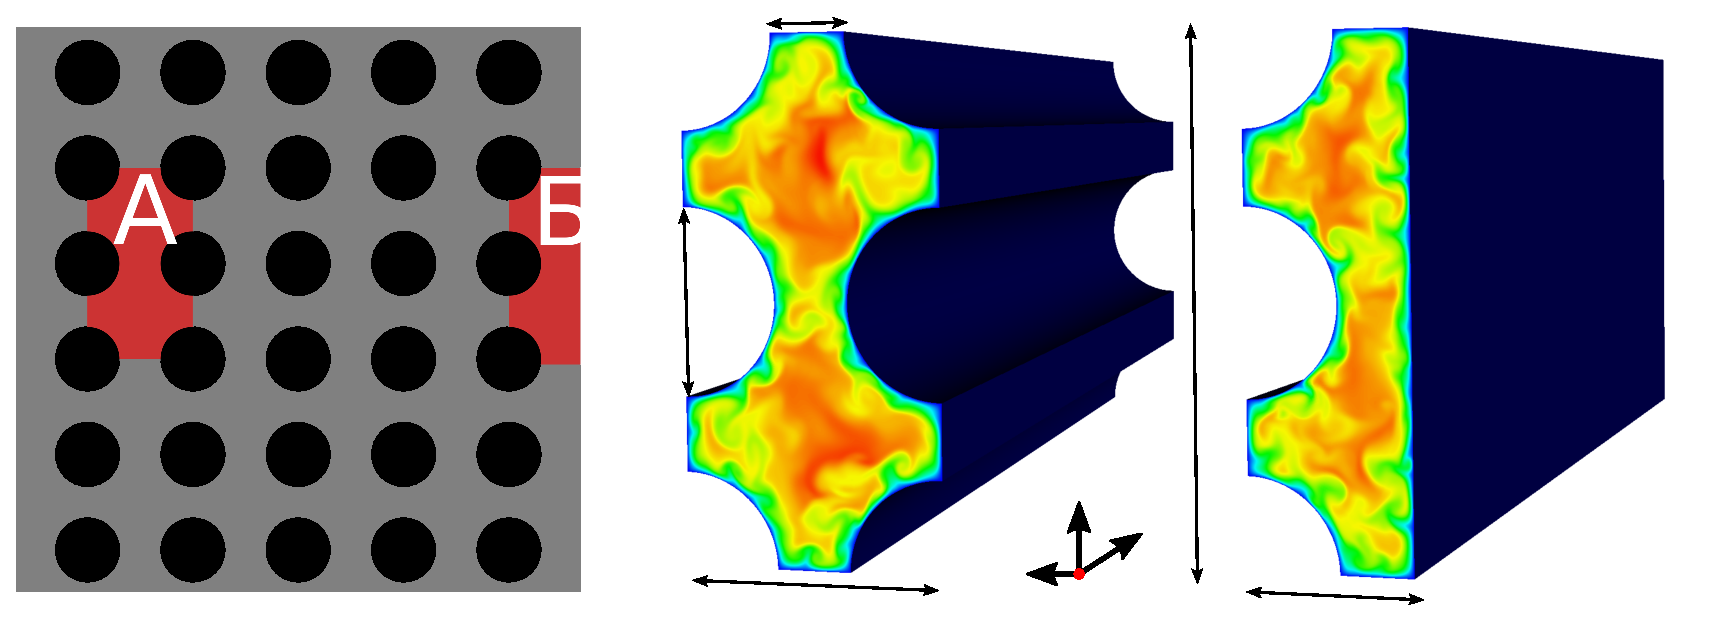
\includegraphics[width=0.9\textwidth]{fig1_new.eps}
  \caption{Модель тепловыделяющей сборки с геометрическими размерами. Черным цветом показаны ТВЭЛы, серым -- теплоноситель. Область типа А -- внутренняя, типа Б -- периферийная.}
  \label{fig:1}
\end{figure}
%


Стоит отметить, что с помощью DNS уже исследовались внутренние конфигурации подобных модельных сборок для различных чисел Рейнольдса [3], но в данной работе упор делается именно на сравнении течения с периферийной областью.
%


\section{Постановка задачи}\label{ch4:problem}
%
На Рис. \ref{fig:1} показаны геометрические модели для расчета двух типов ТВЭЛов: 6-ти внутренних и 3-х периферийных.
%
Диаметр и шаг расположения ТВЭЛов в обоих случаях одинаковы.
%
В дальнейшем условимся обозначать продольное, горизонтальное и вертикальное направления как $(x,y,z)$, соответственно.
%
ТВЭЛы представляют собой цилиндры радиуса 5 мм. с вертикальным и горизонтальным зазорами по 4 мм. между собой. %
Размер в продольном направлении составляет 140 мм., так что продольные когерентные вихревые структуры целиком умещаются в рассматриваемую область.
%
В дальнейшем все результаты приводятся в безразмерном виде, где координаты нормированы на высоту модели ($H=28$ мм.), а скорость на среднерасходную скорость $U_b$.
%


В задаче рассматривается течение жидкости при фиксированном числе Рейнольдса \textit{Re~}$ = 13000$, построенному по гидравлическому диаметру и среднерасходной скорости.
%
Динамика течения полностью описывается уравнениями Навье-Стокса в несжимаемой постановке:
\begin{equation}\label{n-stoks:dimen}
\pfrac{u_i}{t} + u_j \pfrac{u_i}{x_j}= - \pfrac{p}{x_i} + \frac{1}{Re} \pfrac{\tau_{ij}}{x_j},
\end{equation}
%
где $u_i$ - $i$-ая компонента вектора скорости ($i={1,2,3}$), $x_j$ - $j$-ая координата,
%
\begin{equation*}\label{stress:tensor}
\tau_{ij} = \pfrac{u_i}{x_j} + \pfrac{u_j}{x_i}
\end{equation*}
обозначает тензор вязких напряжений.
%
Все величины обезразмерены на характерные значения.
%
$Re = U_b D_h/\nu$ обозначает число Рейнольдса, построенное по среднерасходной скорости и гидравлическому диаметру.

%
Используется два типа граничных условий (ГУ): стенка и периодическое направление.
%
На стенках используется условие прилипания для поля скорости ($u_i = 0$), а также отсутствие поперечного градиента давления ($dp/dn = 0$). 
%
В продольном направлении используются периодические граничные условия для моделирования достаточно длинной ТВС.


\subsection{Вычислительный код и методы дискретизации}
%
Для численного решения уравнений (\ref{n-stoks:dimen}) используется открытый вычислительный код Nek5000, разработанный Полом Фишером и др. [4].
%
Валидация численных алгоритмов была проведена нами ранее на примере различных задач гидродинамики [5,6,7].
%
В его основе лежит метод спектральных элементов (SEM, от англ. Spectral Element Method), по принципу работы схожий с широко известным методом конечных объемов, но в котором решение и данные представлены в виде разложения по многочленам $N$-го порядка в каждом из $E$ деформируемых гексагональных элементов [8].
%
Обычно $N$ варьируется от 8 до 16, так как при использовании меньшего значения $N$ не используются преимущества SEM, а большие значения использовать дорого с вычислительной точки зрения. 
%
В данной работе  $N=10$.
%
SEM отличается малой величиной численной дисперсии и диссипации, что является важным при расчете эволюции гидродинамических неустойчивостей, а также высоких числах Рейнольдса.
%
Спектральная точность означает экспоненциальное уменьшение ошибки с ростом количества вычислительных узлов.
%
Дискретизация по времени происходит при помощи формулы ``дифференцирования назад'' 3-го порядка точности.
%
В рамках пространственной дискретизации в каждом из $E$ элементов переменные задачи раскладываются по базису ${\psi_i}$, состоящему из интерполяционных полиномов Лагранжа:
%
\[
\psi_i(x)=\prod_{j \neq i}\frac{x-\xi_j}{\xi_i-\xi_j}, 
\]
%
где $\xi_i$ - точки, являющиеся корнями уравнения:
\[
(1-\xi^2)\frac{d}{d\xi}P_N(\xi)=0,
\]
в котором $P_N$ - полиномы Лежандра порядка $N$. 
%
Иными словами, $\xi_i$ определяют положение точек сетки внутри спектрального элемента.
%
Более подробно алгоритмы дискретизации и решения уравнений в коде Nek5000 ранее были описаны в книге [9].
%
Вычислительная сетка состоит из порядка 40 млн. узлов для внутренней и 18 млн. узлов для периферийной конфигураций (см. Рис. \ref{fig:3}).
%
Дополнительно была проверена сеточная сходимость для уверенности в достоверности получаемых данных.
%
Также была произведена оценка отношения наименьшего размера вихрей (колмогоровского масштаба)  $\eta_k = (\nu^3/\epsilon)^\frac{1}{4}$, где $\nu$ -- кинематическая вязкость, $\epsilon$ -- скорость диссипации, к шагу сетки $\Delta$.
%
Минимальный шаг сетки оказался сопоставим с колмогоровским масштабом $\Delta_{min} \approx \eta_k$, а максимальный шаг сетки превысил его всего лишь в 3 раза $\Delta_{min} \approx 3\eta_k$, что является хорошим показателем качества вычислительной сетки.

%
\begin{figure}[h!]
  \centering
  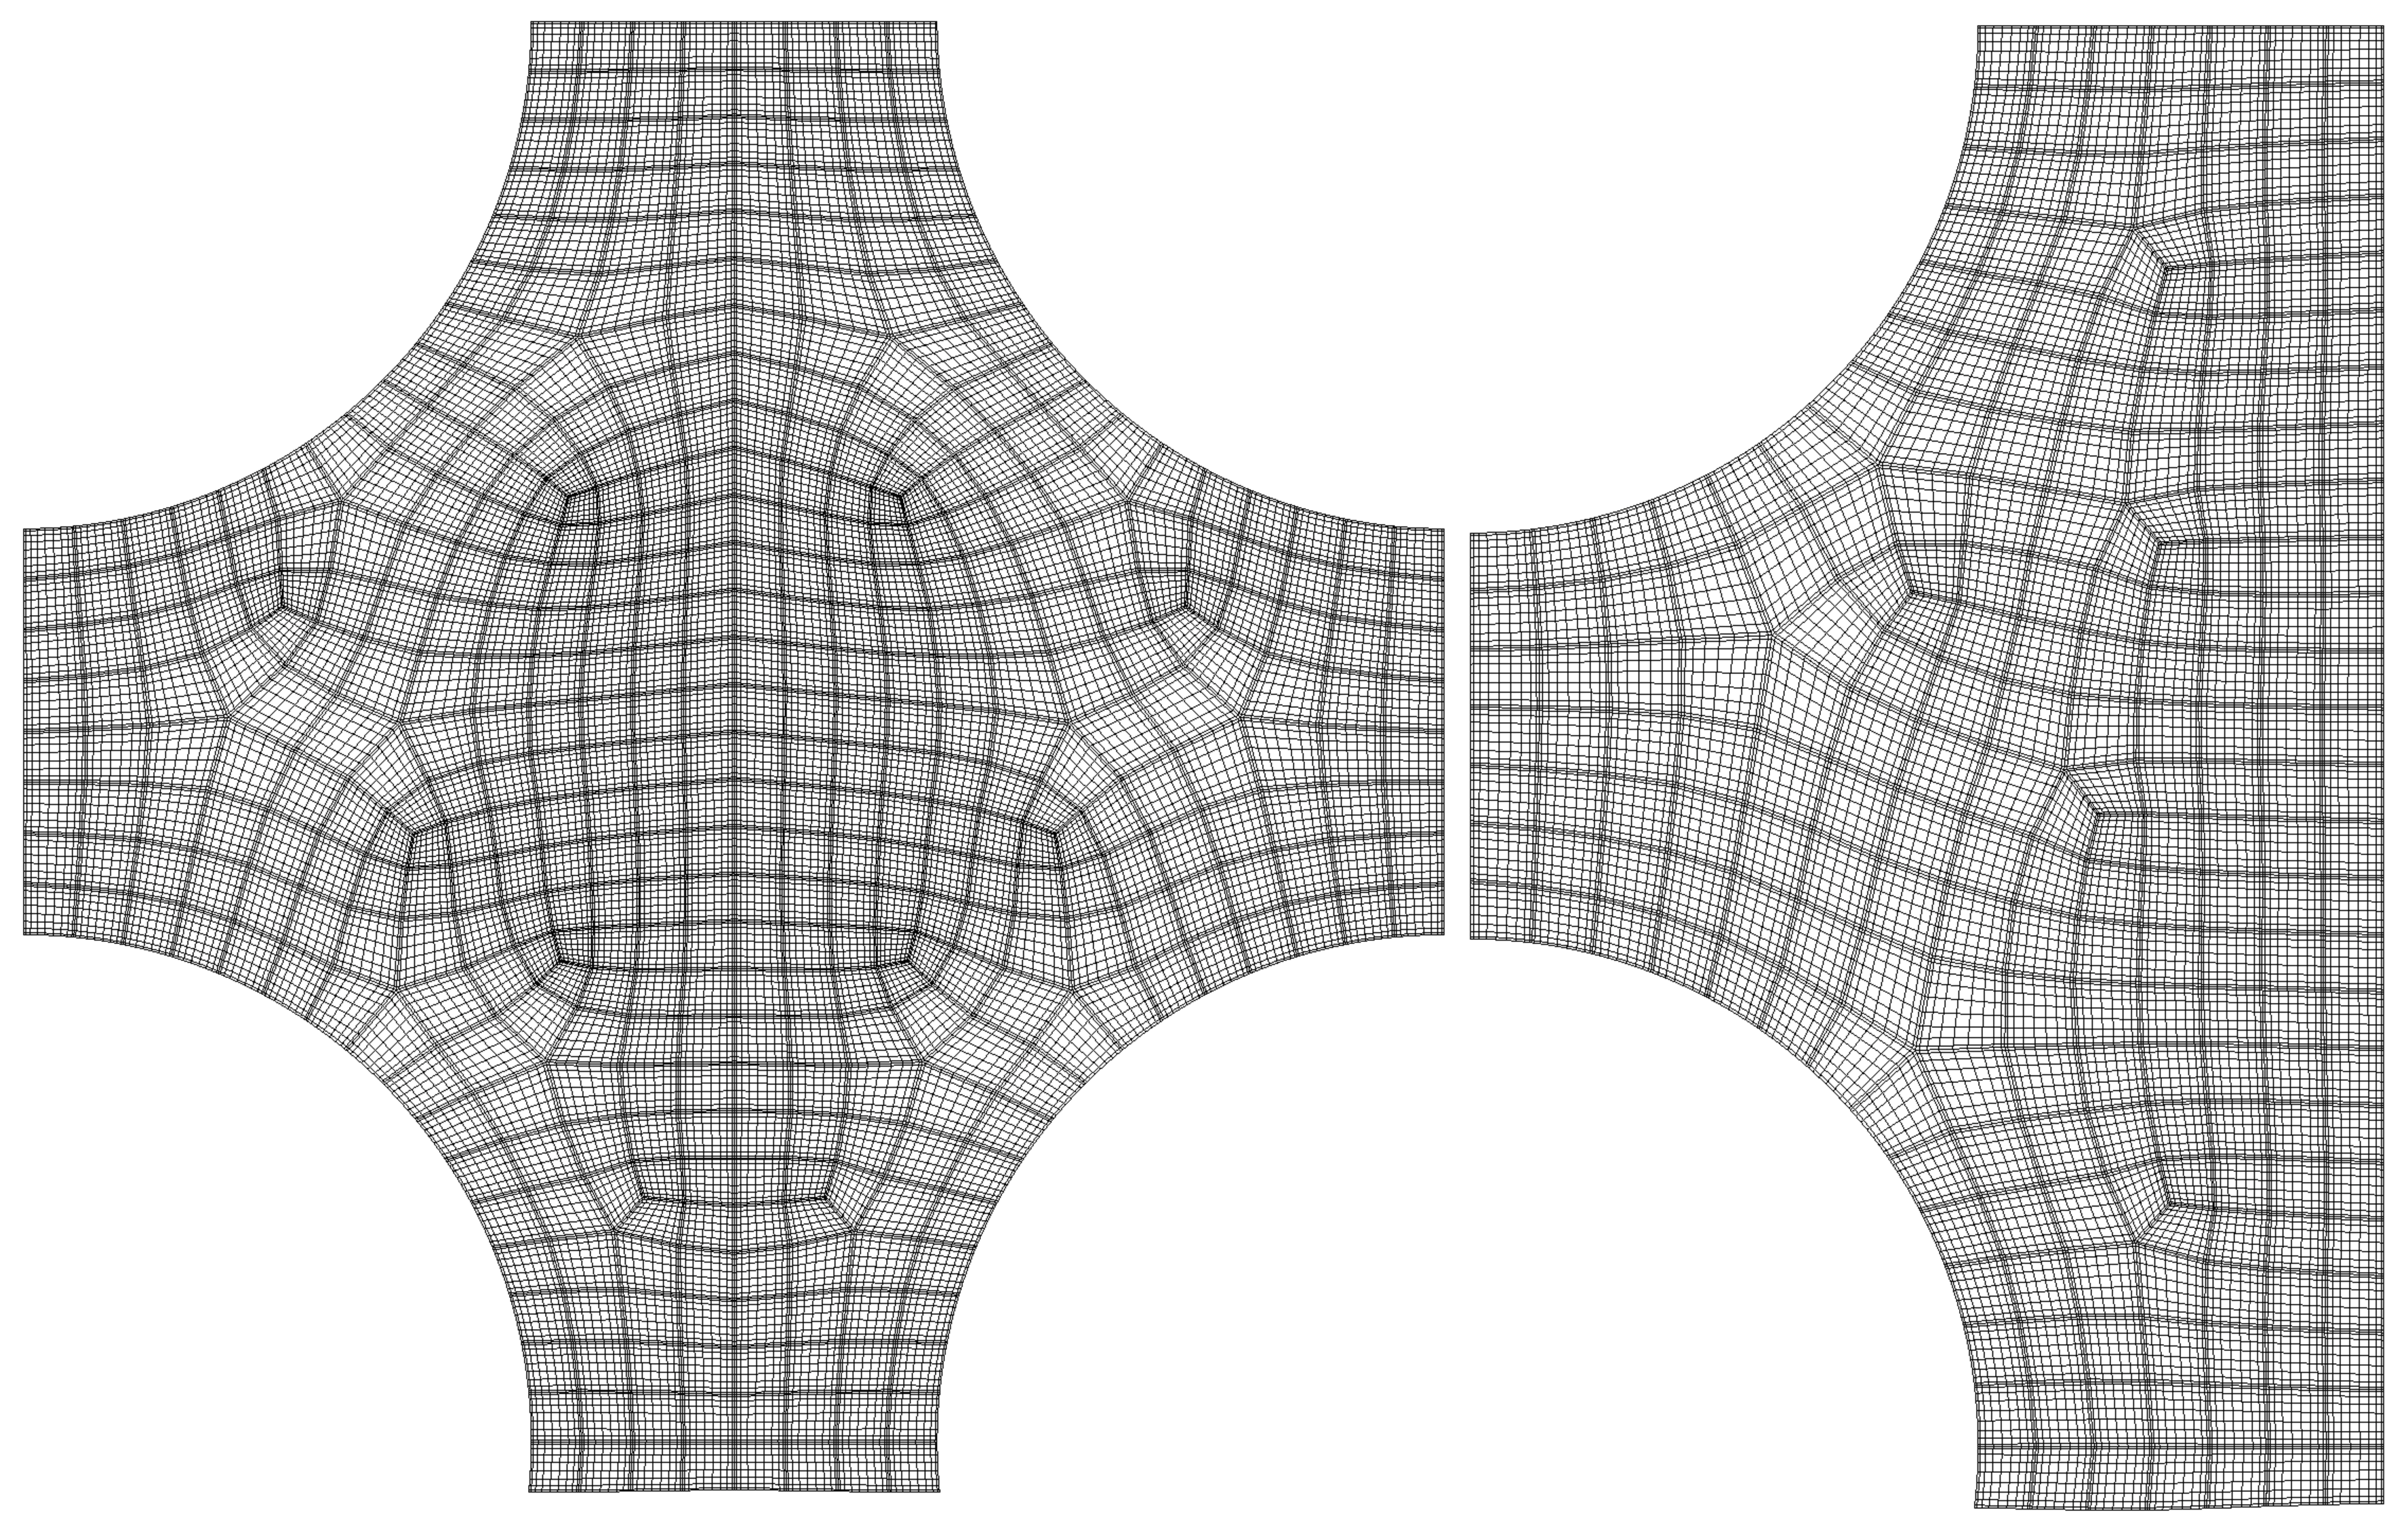
\includegraphics[width=0.5\textwidth]{mesh.eps}
  \caption{Пример вычислительной сетки для поперечного сечения верхней половины геометрии.}
  \label{fig:3}
\end{figure}


\section{Результаты}\label{ch4:results}
На Рис. \ref{fig:4} показано сравнение спектров турбулентной кинетической энергии продольной компоненты скорости ($E_x(fH/U_b)$) в центральных точках обоих конфигураций (отмечены на рисунке). 
%
Турбулентная кинетическая энергия получается с помощью процедуры быстрого преобразования Фурье (FFT, от англ. Fast Fourier Transform): $E_x = |FFT(u'_x)^2|$, где $u'_x = u_x - \overline{u_x}$ -- мгновенные пульсации продольной скорости, а $\overline{u_x}$ -- осредненное по времени поле продольной скорости. 
%
В качестве аргумента используется безразмерная частота $fH/U_b$.

%
Стоит отметить, что в спектрах присутствуют несколько пиков, соответствующих выделенным частотам. 
%
Наличие выделенных частот в потоке соответствует поперечным колебаниям скорости в зазоре, которые связаны с развитием вихревых структур. 
%
Несмотря на то, что в обоих случаях наблюдаются близкие безразмерные частоты, в спектрах уровень кинетической турбулентной энергии выше в случае периферийной конфигурации.
%
При этом на Рис. \ref{fig:4} пунктирными линиями также показаны горизонтальное и вертикальное сечения, в которых проводилось сравнение профилей средней продольной скорости и ненулевых компонент тензора напряжений Рейнольдса, показанное на Рис. \ref{fig:5}.

% Видно, что для обоих случаев спектры очень близки, при этом характерные безразмерные частоты на спектре также отличаются незначительно: 0.39 для внутренней конфигурации и 0.37 для периферийной. 
%


\begin{figure}[h!]
  \centering
  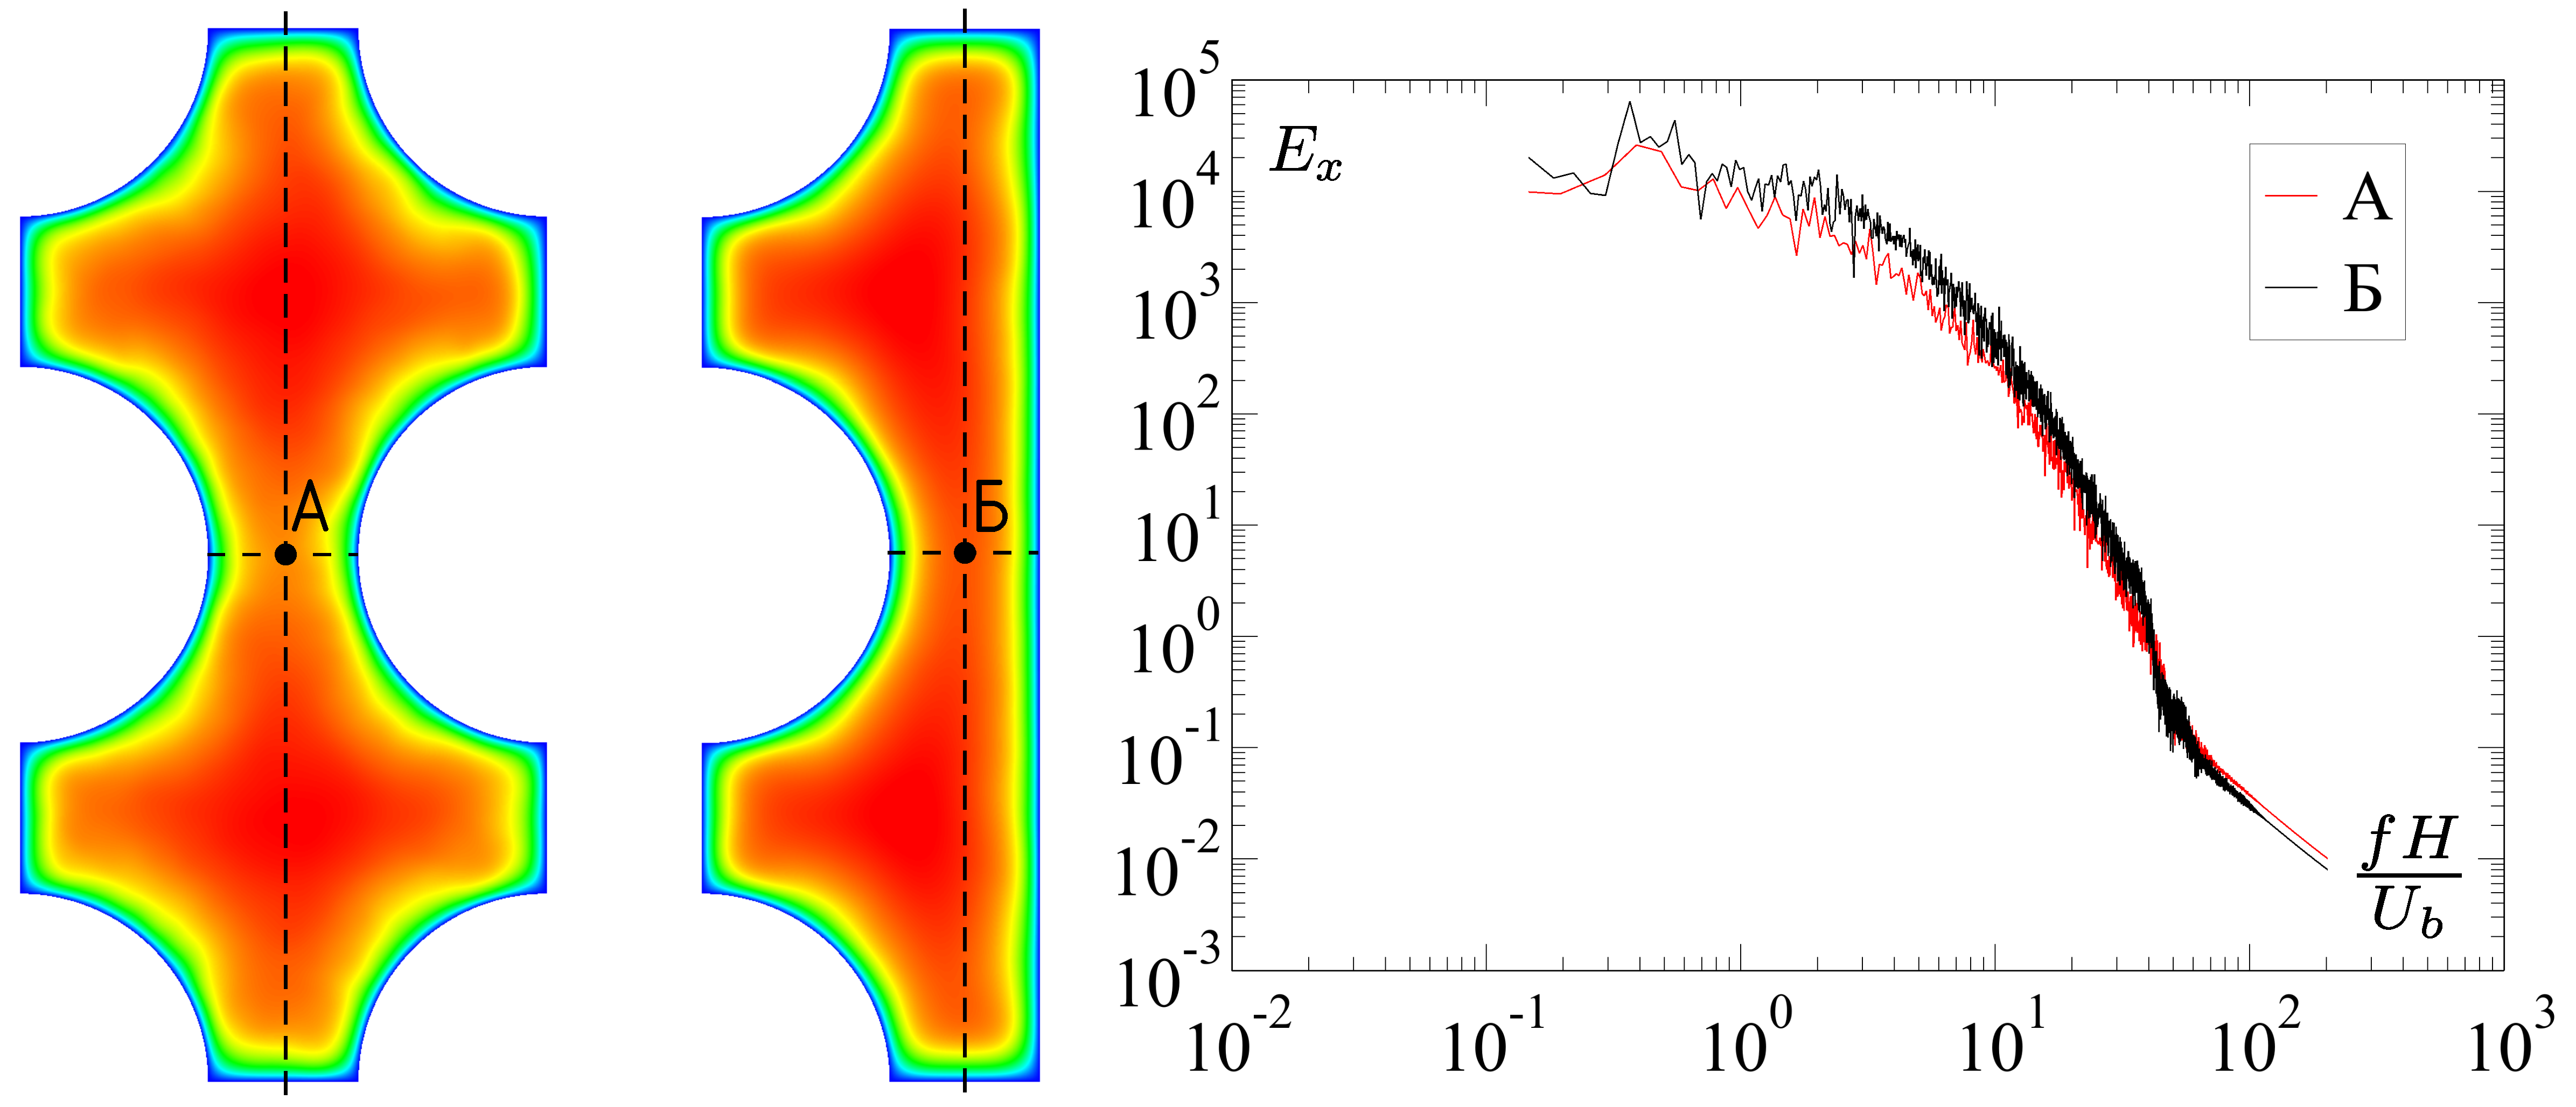
\includegraphics[width=0.9\textwidth]{spectres.eps}
  \caption{Спектры турбулентной кинетической энергии для двух конфигураций. Пунктирными линиями показаны сечения, в которых сравниваются средние профили скорости и пульсаций на Рис. \ref{fig:5}}
  \label{fig:4}
\end{figure}

%
%
%
На Рис. \ref{fig:5}\textit{а} и \ref{fig:5}\textit{б} приведен профиль продольной скорости вдоль горизонтального и вертикального сечения, соответственно.
%
Горизонтальная координата нормирована на ширину межтвэльного пространства $\delta = 4$ мм., вертикальная -- на высоту модели $H = 28$ мм.
%
В межтвэльном пространстве наблюдается неплохое совпадение результатов (с точностью до 7\%), хотя в точках $z/H = 0.25$ и $z/H = 0.75$ наблюдается наибольшее различие в графиках из-за наличия плоской стенки в периферийной конфигурации и, как следствие, изменения структуры вторичных течений.
%
На рисунках \ref{fig:5}\textit{в} -- \ref{fig:5}\textit{е}, несмотря на довольно высокое отклонение профилей друг от друга, наблюдается качественное совпадение профилей для обоих конфигураций.
%
При этом стоит отметить, что наибольшие отклонения наблюдаются для наименее интенсивных компонент тензора напряжений Рейнольдса, которые вносят наименьший вклад в общую турбулентную кинетическую энергию.


%
% \begin{figure}[h!]
%   \centering
%   \includegraphics[width=0.9\textwidth]{profiles.eps}
%   \caption{Профили ненулевых компонент тензора напряжений Рейнольдса и средней продольной скорости для двух рассмотренных конфигураций. Красным цветом показаны результаты для внутренней сборки, черным -- для периферийной. Горизонтальная ось соответствует расстоянию $y/H$ вдоль пунктирной линии, показанной на Рис. \ref{fig:4}}.
%   \label{fig:5}
% \end{figure}
%
\begin{figure}[h!]
  \centering
  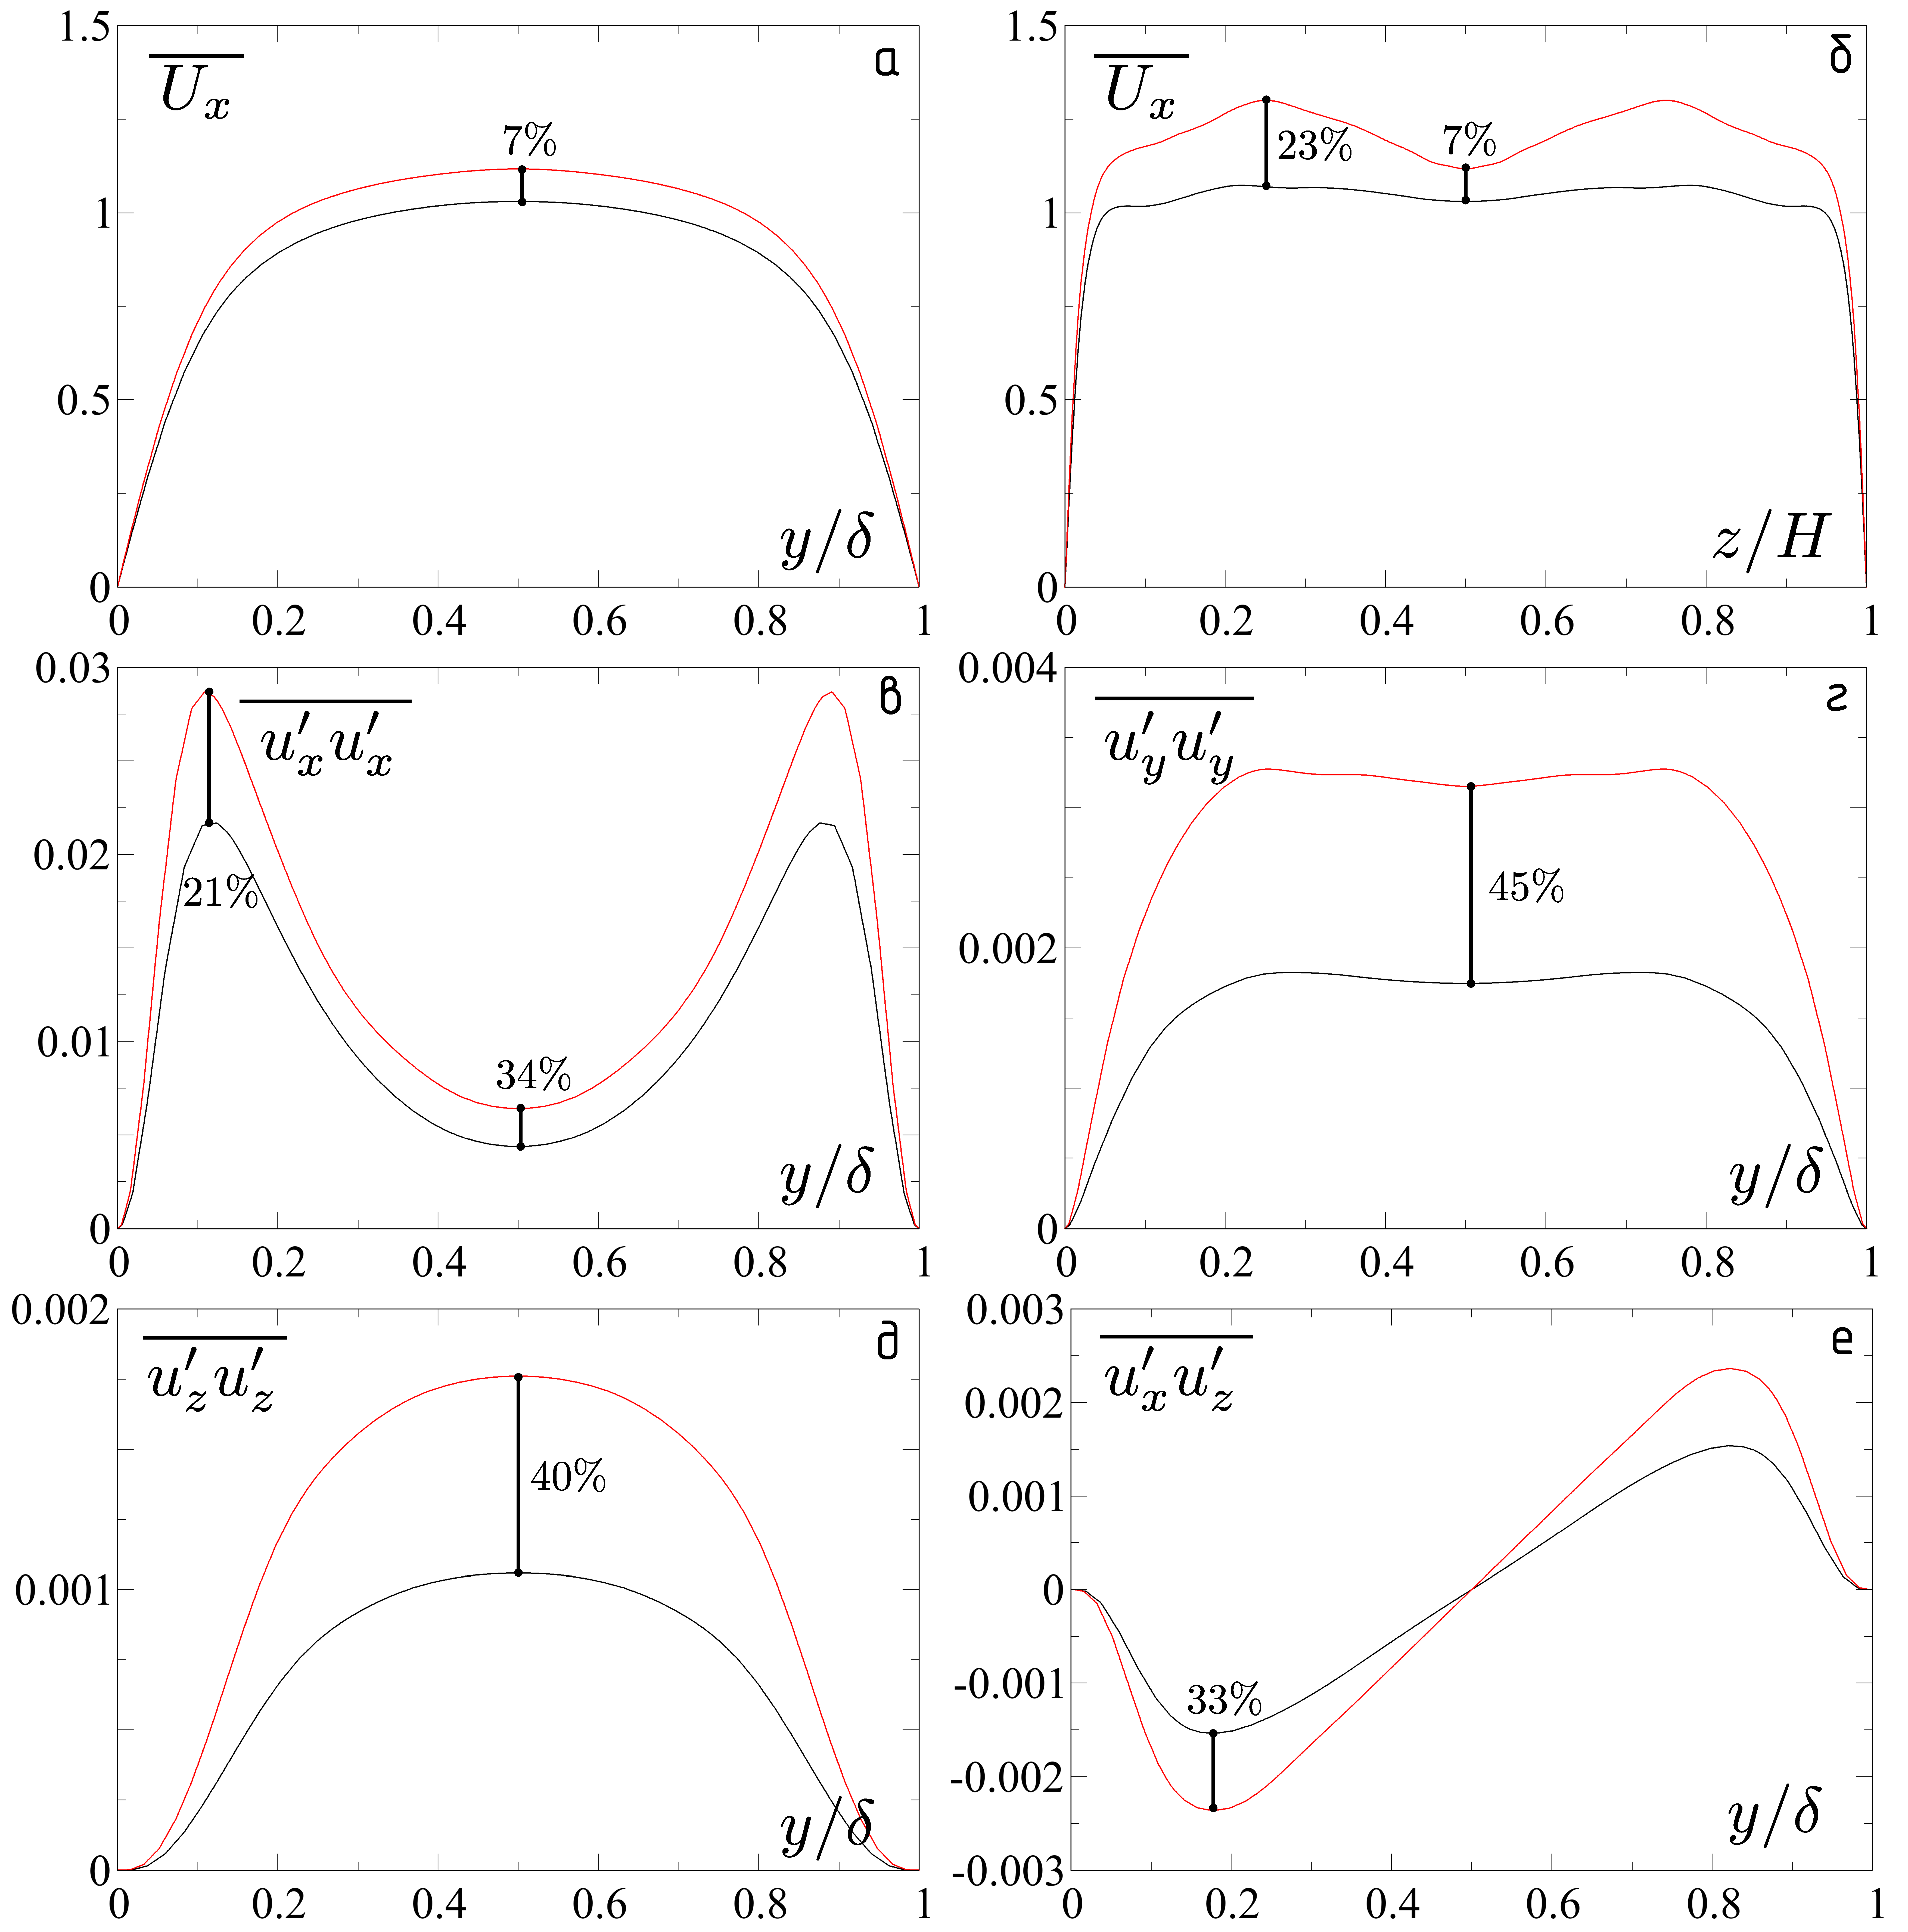
\includegraphics[width=0.9\textwidth]{profiles_mid.eps}
  \caption{Профили ненулевых компонент тензора напряжений Рейнольдса и средней продольной скорости для двух рассмотренных конфигураций. Красным цветом показаны результаты для внутренней сборки, черным -- для периферийной. Горизонтальная ось соответствует расстоянию $y/H$ вдоль пунктирной линии, показанной на Рис. \ref{fig:4}}.
  \label{fig:5}
\end{figure}





\section{Выводы}\label{ch4:conclusion}
%
Было проведено прямое численное моделирование двух модельных областей сборок ТВЭЛов: внутренней и периферийной. 
%
Выявлено, что профили средней скорости, а также компонент тензора напряжений Рейнольдса имеют качественные сходства для обоих конфигураций. 
%
Наибольшие отклонения наблюдаются в наименее интенсивных компонентах тензора напряжений Рейнольдса, вследствие чего на спектре турбулентной кинетической энергии явных различий выявлено не было, что дает возможность предполагать о незначительном влиянии плоской стенки на процессы переноса энергии в межтвэльном пространстве. 
%
При этом основные отличия между конфигурациями вызваны изменением структуры вторичных течений (для внутренней области они намного интенсивнее), что и приводит к изменению пульсационных характеристик.
%
Таким образом можно установить, что экспериментальные результаты при исследовании периферийной области сборки ТВЭЛов качественно отражают картину турбулентного течения и для внутренней части сборки, однако влияние найденных различий в профилях компонент тензора напряжений Рейнольдса на процессы теплопереноса требует дальнейшего детального изучения.

           % Глава 4
\chapter*{Заключение}                       % Заголовок
\addcontentsline{toc}{chapter}{Заключение}  % Добавляем его в оглавление

%% Согласно ГОСТ Р 7.0.11-2011:
%% 5.3.3 В заключении диссертации излагают итоги выполненного исследования, рекомендации, перспективы дальнейшей разработки темы.
%% 9.2.3 В заключении автореферата диссертации излагают итоги данного исследования, рекомендации и перспективы дальнейшей разработки темы.
%% Поэтому имеет смысл сделать эту часть общей и загрузить из одного файла в автореферат и в диссертацию:

Основные результаты работы заключаются в следующем.
%% Согласно ГОСТ Р 7.0.11-2011:
%% 5.3.3 В заключении диссертации излагают итоги выполненного исследования, рекомендации, перспективы дальнейшей разработки темы.
%% 9.2.3 В заключении автореферата диссертации излагают итоги данного исследования, рекомендации и перспективы дальнейшей разработки темы.
\begin{enumerate}
  \item На основе данных прямого численного моделирования показана зависимость вероятности образования
  пристеночных обратных течений от нагрева стенок квадратного турбулентного канала, а также качественные различия 
  в наблюдаемых явлениях в зависимости от степени нагрева
  \item Численные исследования показали, что устройства-реламинаризаторы с хорошей точностью можно моделировать
  с помощью локального увеличения вязкости. При этом получаемые результаты хорошо согласуются с экспериментальными 
  данными, полученными другими авторами
  \item Продемонстрировано несущественное отличие между внутренней и периферийной областями тепловыделяющей
  сборки с точки зрения экспериментально получаемых данных
  \item Исследованы процессы теплоотвода с поверхности ТВС с помощью свинцово-висмутового сплава жидких металлов
\end{enumerate}



\textbf{Благодарности} 
Автор благодарит Институт теплофизики СО РАН и Новосибирский государственный университет за 
предоставленные вычислительные ресурсы суперкомпьютера ``Каскад''.
Также автор выражает благодарность и большую признательность научному руководителю
Мулляджанову Р.И. за поддержку, помощь, обсуждение результатов и научное руководство.
Также автор благодарит Зарипова Д.И. за поддержку, помощь в анализе научных результатов и 
совместную работу, Палкина Е.В. и Иващенко Е.И. за помощь в работе в вычислительном пакете Nek5000.      % Заключение
\include{Dissertation/acronyms}        % Список сокращений и условных обозначений
\include{Dissertation/dictionary}      % Словарь терминов
\include{Dissertation/references}      % Список литературы
\include{Dissertation/lists}           % Списки таблиц и изображений (иллюстративный материал)

\setcounter{totalchapter}{\value{chapter}} % Подсчёт количества глав

%%% Настройки для приложений
\appendix
% Оформление заголовков приложений ближе к ГОСТ:
\setlength{\midchapskip}{20pt}
\renewcommand*{\afterchapternum}{\par\nobreak\vskip \midchapskip}
\renewcommand\thechapter{\Asbuk{chapter}} % Чтобы приложения русскими буквами нумеровались

% \include{Dissertation/appendix}        % Приложения

\setcounter{totalappendix}{\value{chapter}} % Подсчёт количества приложений

\end{document}
